\chapter{Model-Experiment-Exercises (MEX)}

The basic idea of Model-Experiment-Exercises (MEX) is to link modelling and experimental works from the very beginning – i.e. in the conceptual phase. Due to the complexity of each part in the systems analysis, this combination is sometimes lost. Moreover, both models and experiments require highly sophisticated tools and equipment as well as highly specialized professionals, which also necessitate adequate measures and incentives for collaboration. GeomInt is introducing the MEX concept exactly for this purpose. Therefore, the following MEX studies occupy the largest part of the GeomInt book and feed most of the publications with research material.

\begin{wrapfigure}{l}{5cm}
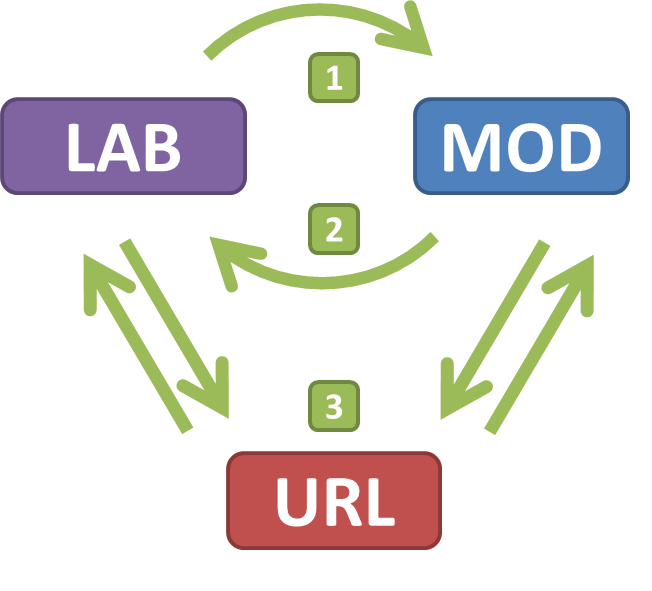
\includegraphics[width=4.9cm]{figures/geomint-mex-a}
\caption{MEX concept}
\label{fig:mex-concept-generic}
\end{wrapfigure}
In order to illustrate the MEX concept, Fig. \ref{fig:mex-concept-generic} depicts the dependencies between laboratory (LAB) and field experiments (URL) as well as modelling work (MOD). Lab experiments (LAB) will be analysed by models (MOD) in order to calibrate parameters and validate them [1]. This step in the analysis loop should proof that the models are able to represent the experiments (validation). Models will be also used for planning experimental work in order to improve the general process understanding [2] (experimental design). Both lab experiments and models must be scaleable to field experiments [3].

\begin{figure}
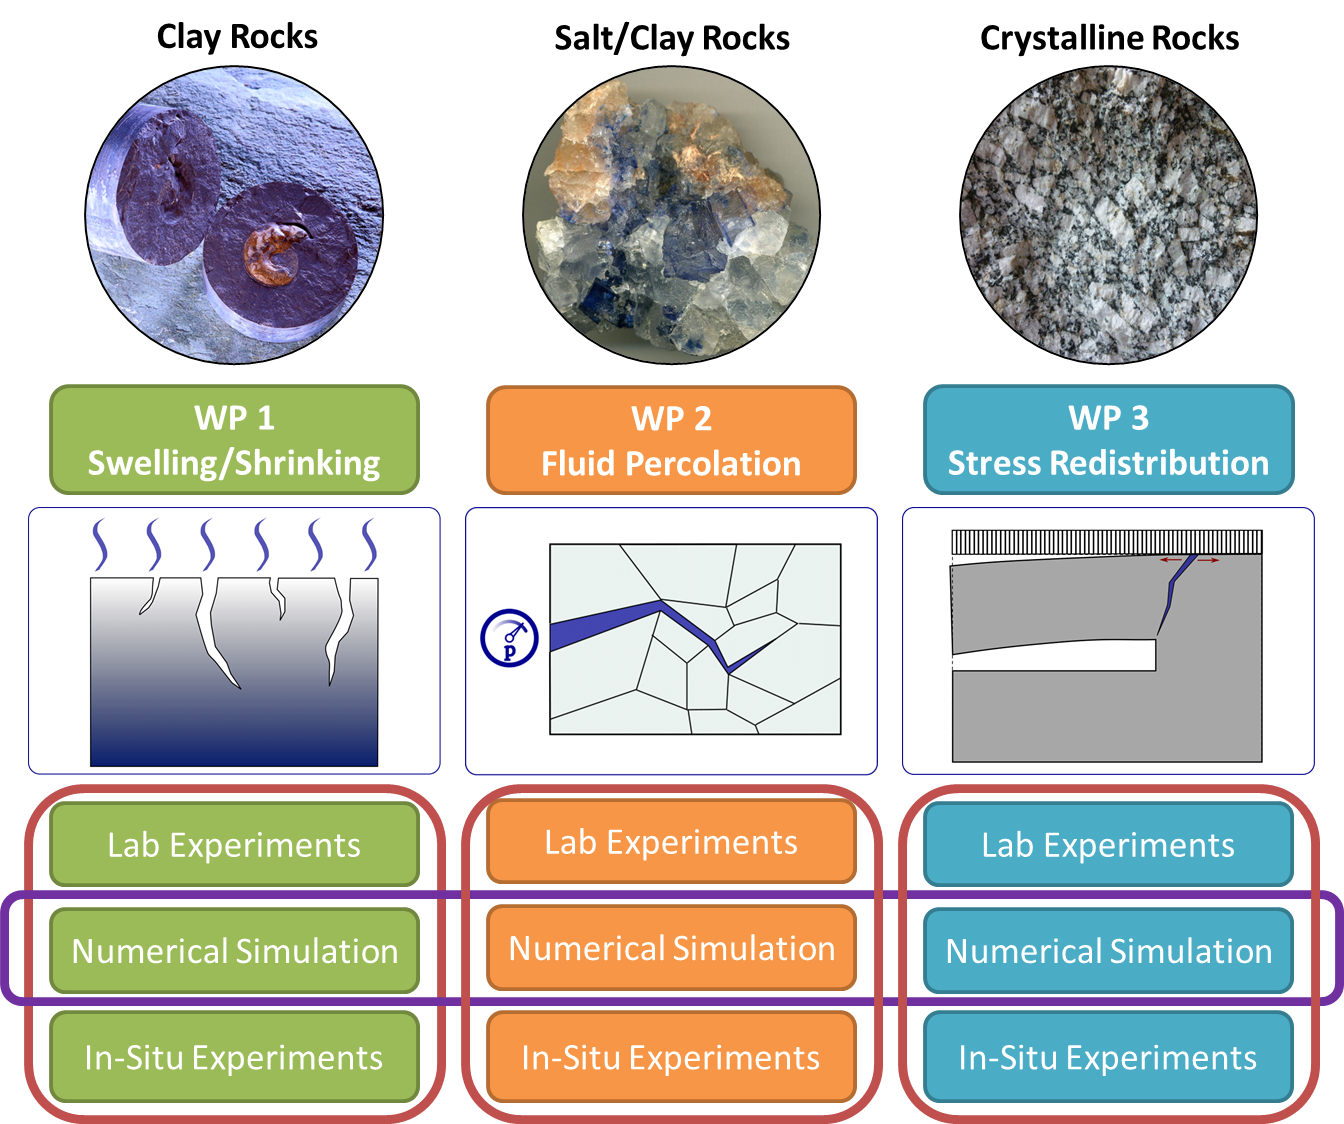
\includegraphics[width=0.85\textwidth]{figures/geomint-mex-b.png}
\caption{MEX in WPs}
\label{fig:mex-concept-wps}
\end{figure}

The generic approach for systems analysis described above is applied to GeomInt through the individual work packages (WP1-3) linking experimental works in the laboratories (lab and field) and numerical modelling (Fig. \ref{fig:mex-concept-wps}). Due to the limited project time this is being demonstrated for selected cases. A specific challenge for the GeomInt project is the development and implementation of generic numerical methods which are able to simulated THM coupled processes for various rock types – ductile and brittle materials (thermodynamic consistency) with an emphasis of discontinuities. This is the concept of building GeomInt frameworks – experimental (see Chapter \ref{cha:exp}) and numerical platforms (see Chapter \ref{cha:num}).

Before WP related MEX are described, a prerequisite of two exercises dealing with bending test are introduced for granite and clay. Here the fracture process is initiated by external loads (i.e. not by fluid injection). These bending tests are providing important information on the elastic material behavior before fracturing the specimen (MEX01). Moreover, for clay samples, particularly from sandy facies, the lamination of the material is largely influencing fracturing processes. A concept for a humidity controlled bending test is presented in MEX13 with is related to the planned CD-A experiment in Mt. Terri.

\clearpage
\begin{figure}[hbtp]
\caption{Model-Experiment-Exercises (MEX) as of 27.12.2019}
\centering
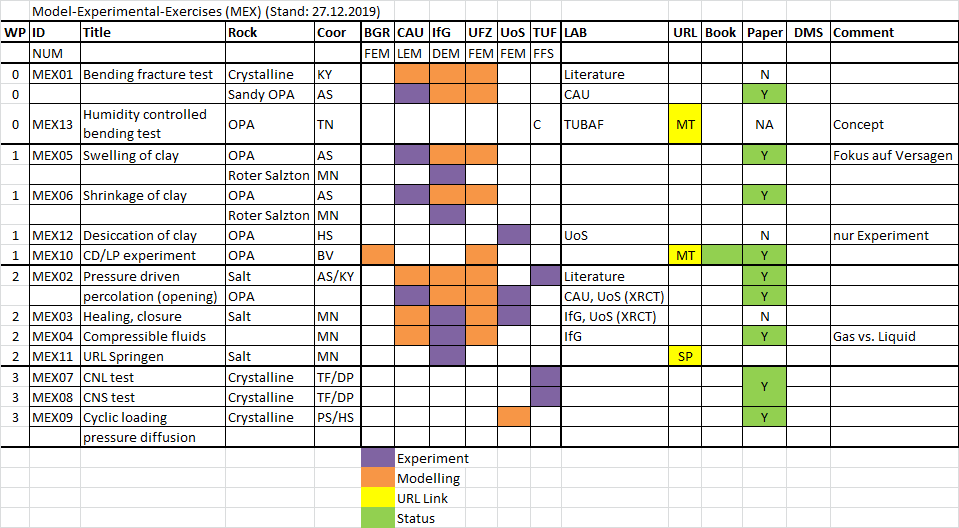
\includegraphics[width=18cm,angle=90]{figures/mex-overview.png}
\end{figure}

\clearpage
%------------------------------------------------------------------------------
%\section{Model Exercise 0-1a (01): Bending fracture test}
\label{sec:mex01}
%------------------------------------------------------------------------------
\Authors{Keita Yoshioka, Amir Shoarian Sattari, Mathias Nest et al.}
%------------------------------------------------------------------------------
\subsection{Experimental set-up}
%------------------------------------------------------------------------------
Model Exercise 1 (ME 1) is concerned with fracture propagation by external loads (i.e. without internal hydraulic force). Experimental data are taken from Three Point Bending (TPB) tests conducted on Rockville Granite samples \cite{Tarokh2016161}. TPB experiments are performed by applying a load on the top of the samples and the load is adjusted by keeping the rate of the Crack Mouth Opening Displacement (CMOD) fixed at 0.05 $\mu$m/s.
The schematic of TPB is shown in Figure \ref{fig:ME1_TPB_experiment}.

\begin{figure}[!ht]
\centering
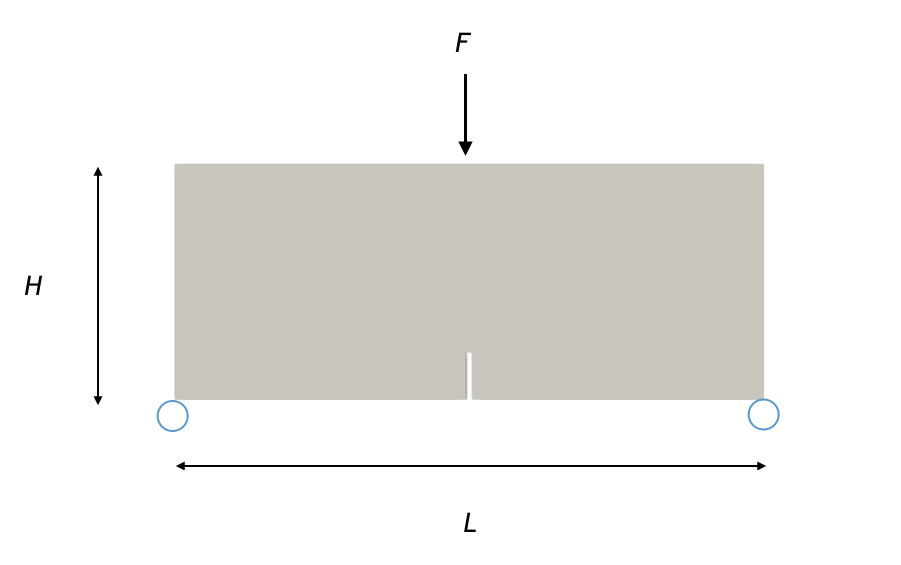
\includegraphics[width=1\textwidth]{figures/TPB_exp.png}
\caption{Three Point Bending experimental set up}
\label{fig:ME1_TPB_experiment}
\end{figure}

The width of the notch is 1.2 mm at the center of the sample and the ratio of notch length to the sample height is 0.2. 
Other parameters used for simulation are listed in Table \ref{table:ME1_TPB_experiment}.

\begin{table}[!ht]
\centering
\begin{tabular}{c c c |c c c c}
$w$ & $L$ (span) & $H$ & $E$ &  $\nu$ &  UCS  & $\sigma_T$  \\
\hline
30 mm & 127 mm & 50.8 mm  & 27.5 GPa & 0.175 & 106 MPa &  8.1 MPa \\
\end{tabular}
\caption{Parameters used for the simulation of Three Point Bending tests. 
\label{table:ME1_TPB_experiment}
}
\label{tabl:Numerical_param_for_sneddon_crack}
\end{table}
The experimental force-displacement results from cite Tarokh for two samples are shown in Figure \ref{fig:ME1_TPB_force_disp}.

\begin{figure}[!ht]
\centering
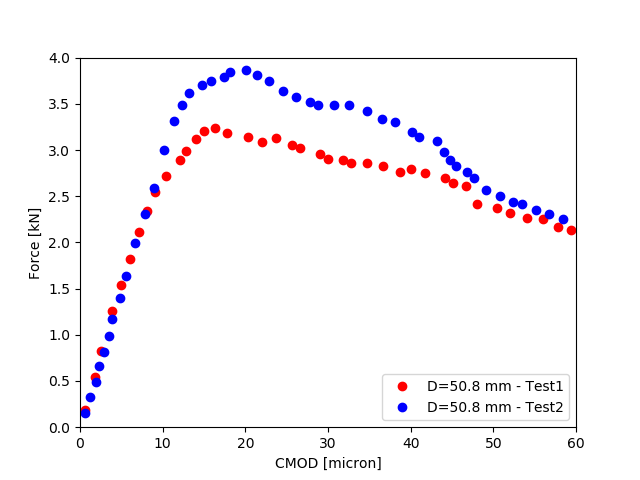
\includegraphics[width=1\textwidth]{figures/TPB_Force_Disp.png}
\caption{Three Point Bending test results.}
\label{fig:ME1_TPB_force_disp}
\end{figure}
%------------------------------------------------------------------------------
\subsection{Model approach}
%------------------------------------------------------------------------------
\subsubsection*{Discrete-Element-Model (DEM)}

Two models were set up to represent granite samples with different grain structures. As reported in reference \cite{Tarokh2016161}, the average grain size of the Rockville granite in the experiment was 10 mm. 
As they are embedded in more finely grained material, a discrete element model with a Voronoi-block diameter of 5.4 mm has been chosen. For the Voronoi-discretization random points were inserted in the sample volume. 
The serve as the center coordinates of the Voronois. After 10$^5$ insertion attempts, this lead to 1236 grains for the first sample, and 1226 for the second sample, see Fig. \ref{fig:ME1_TPB_DEM_domain}. Finally a notch was cut from the models. The behaviour of the model follows from the properties of both the grains (bulk modulus $K$ and shear modulus $G$), and the interface parameters (normal stiffness $k_n$, shear stiffness $k_s$, and tensile strength $\sigma_z$). These can be combined in several ways to reproduce the experimental results in Fig. \ref{fig:ME1_TPB_force_disp}. In this model we have chosen $K$ = 14.1 GPa, $G$ = 11.7 GPa, $k_n$ = 1700 GPa/m, $k_s$ = 170 GPa/m, and $\sigma_z$ = 2.5 MPa. 

\begin{figure}[!ht]
\centering
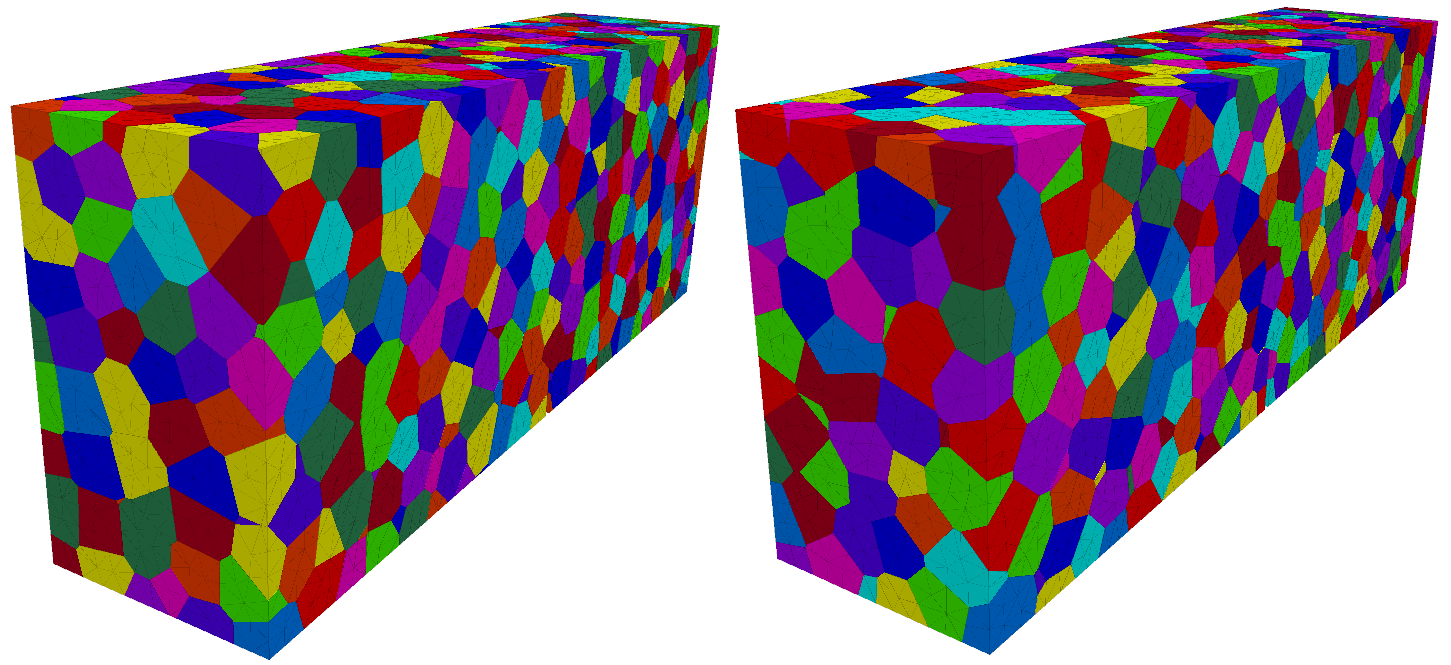
\includegraphics[width=1\textwidth]{figures/ME1-DEM-samples.png}
\caption{Discrete element model computation domain}
\label{fig:ME1_TPB_DEM_domain}
\end{figure}

\subsubsection*{Lattice-Element-Model (LEM)}

The lattice element method (LEM) with the refined mesh is implemented to model the three-point bending test according to the experimental data given in Table \ref{table:ME1_TPB_experiment}. The regularization of the parameters is carried out to assure the mesh independence results (Section \ref{Section:MechanicalLattice}). The total number of the elements is around 500,000 elements, where the mesh distance in the refined domain is 1.2mm, granting the experimental notch width (Figure \ref{fig:Amir_ME1_LEM_Setup}). The considered Young Modulus is 35GPa to match the experimental linear elastic response.

\begin{figure}[!ht]
\centering
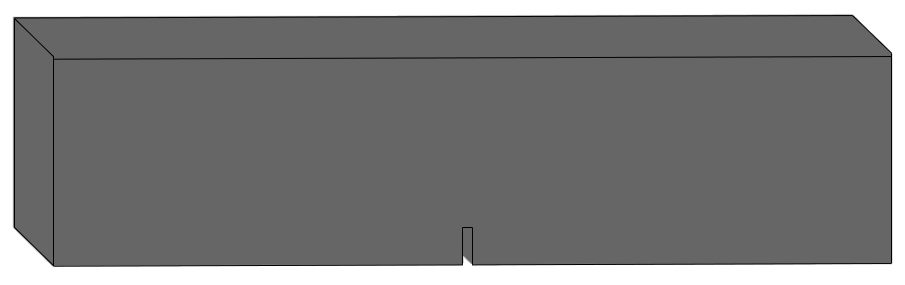
\includegraphics[width=11cm,height=5cm]{figures/Amir_ME1_LEM_Setup.png}
\caption{The lattice setup for the simulation of the fracture toughness}
\label{fig:Amir_ME1_LEM_Setup}
\end{figure}


\subsubsection*{Finite-Element-Model: Variational Phase-Field (VPF)}

The finite element mesh constructed for the 50.8 mm test is shown in Fig.~\ref{fig:ME1_TPB_VF_domain}, which consists of 1,682,308 three dimensional tetrahedral elements with 316,636 nodes.
The notch with the width of 1.2 mm is explicitly meshed in the domain and the top load is applied at the row of the nodes on the top.
The average tetrahedral size is 0.3 mm, which is 1/4 of the notch width, in the refined region.
The Young's modulus in the simulation was increased to 40 GPa from the one listed in Table~\ref{table:ME1_TPB_experiment} in order to match the linear elastic response. 
Another property required in the variational phase-field model is the fracture toughness rather than macroscopic yield strengths as the methodology is based on fracture mechanics.
The fracture toughness, $G_c$ of 35 Pa-m was chosen to match the peak force from the experiment.

\begin{figure}[!ht]
\centering
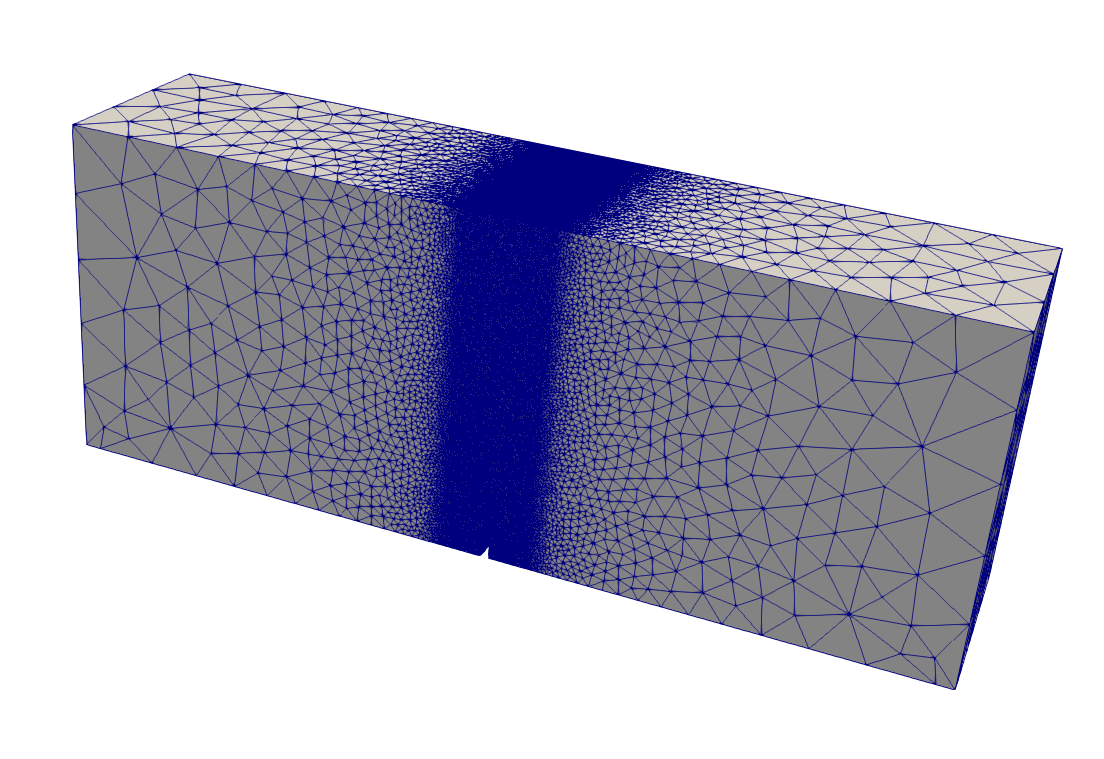
\includegraphics[width=1\textwidth]{figures/VPF_model_domain_mesh.png}
\caption{Variational phase-field computation domain}
\label{fig:ME1_TPB_VF_domain}
\end{figure}

\begin{figure}[!ht]
\centering
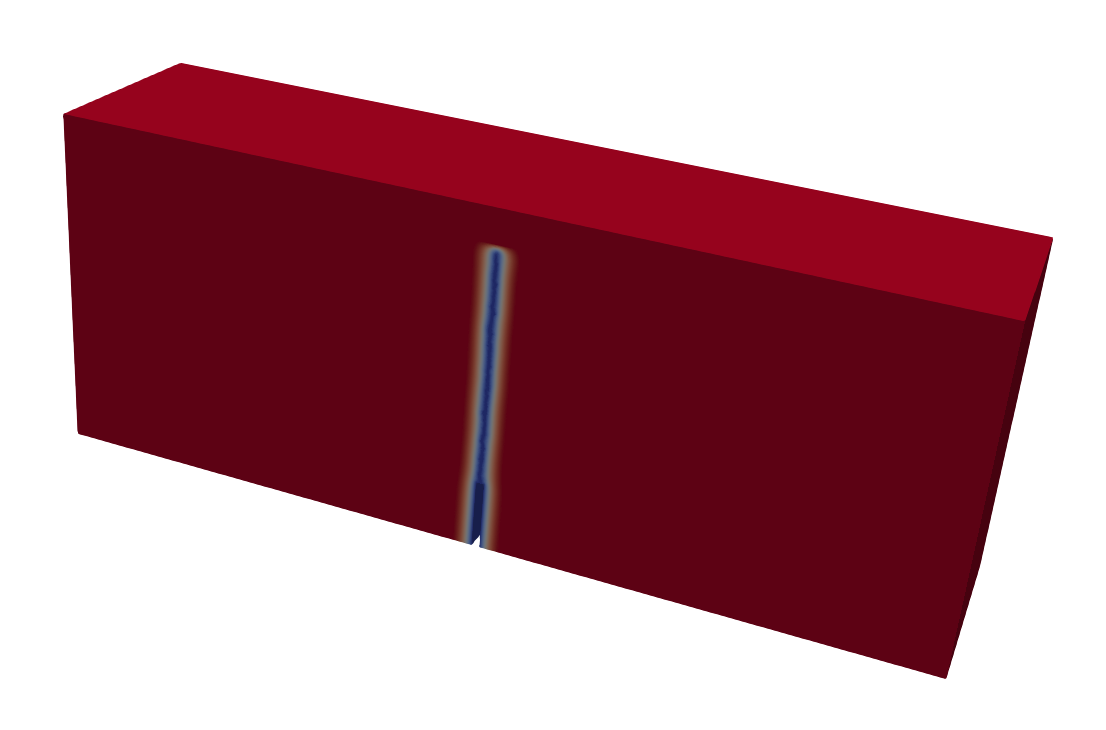
\includegraphics[width=1\textwidth]{figures/VPF_ME1_frac.png}
\caption{Variational phase-field computation result}
\label{fig:ME1_TPB_VPF_result}
\end{figure}

%------------------------------------------------------------------------------
\subsection{Results and discussion}
%------------------------------------------------------------------------------
Simulation results from all the simulations are shown in \ref{fig:ME1_comparison}. 
All the models exhibit linear elastic behaviors, before failure sets in as in the experimental data.
First, we can see that all the models reproduce the linear elastic response.
It is straightforward for the variational phase-field model as it only requires the descriptions of the linear elastic properties (i.e. the Young's modulus and the Poisson's ratio).
However, for the lattice or discrete element methods, these bulk properties need to be obtained through the micro mechanical properties. In lattice method the strain energy stored in unit cell should be equal to the continuum strain energy. Therefore, for a Euler Bernoulli beam elements and while considering 
the stored energies, the micro to macro (bulk) transformation of properties is carried out, see \cite{Ostojastarzewski2002}.

The main difference between the discrete/lattice element method and the variational phase-field model is the responses after the failure.
While the current implementation in the variational phase-field used in this study is based on the linear elastic brittle fracture mechanics, and plasticity or softening is not 
considered \footnote{The linear elastic fracture mechanics formulation is not necessary constrained by the variational phase-field formulation. Models that include ductility, plasticity, 
and softening behaviors exist. For example, see \cite{Alessi2018}}.
For this reason, the result from the variational phase-field model fails elastically and the force ceases to zero quickly after the peak.
On the other hand, the lattice and discrete element methods can model a softening of the bulk material. The implemented softening 
scheme in lattice element is based on bi-linear softening behavior found in \cite{Inceetal2003}.
This post-failure behavior agrees with the real rock response better than the approach based on the linear elastic fracture mechanics.

\begin{figure}[!ht]
\centering
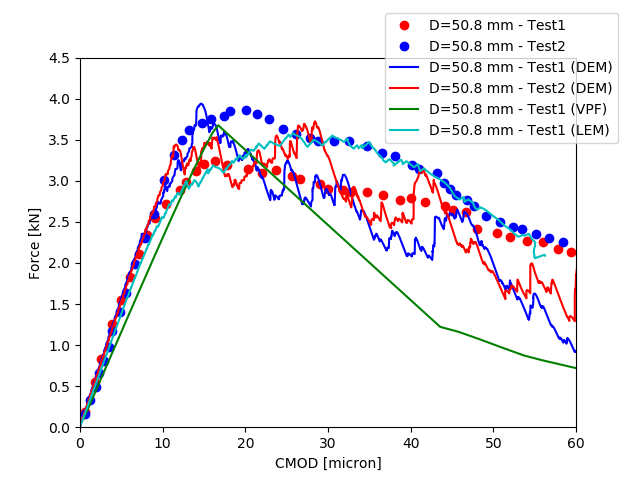
\includegraphics[width=1\textwidth]{figures/ME1_comp_updated.png}
\caption{Model comparison}
\label{fig:ME1_comparison}
\end{figure}

All three methods reproduce a similar pattern of horizontal displacements. The VPF ... The result from the DEM is shown in Fig. \ref{fig:ME1-xdis-dem}. 
The crack does not extend quite as far as in the VPF method, but the absolute extend ... 

\begin{figure}[!ht]
\centering
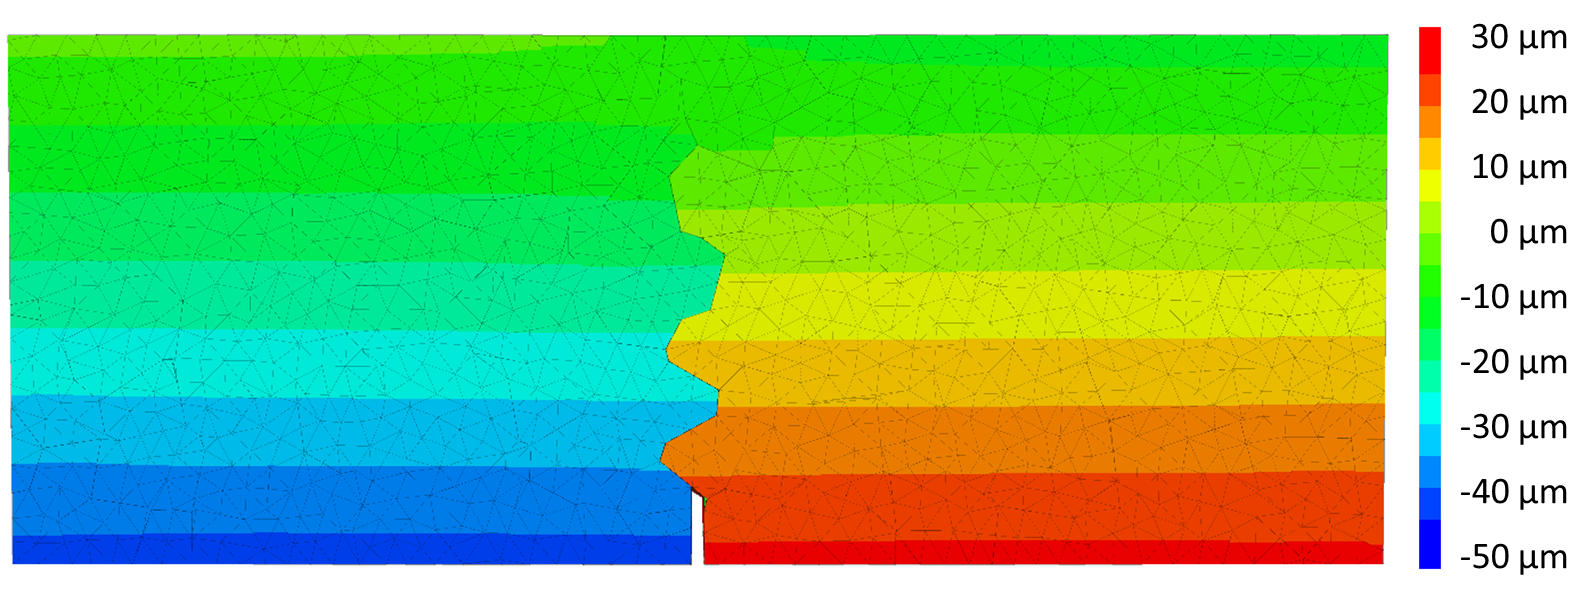
\includegraphics[width=1\textwidth]{figures/ME1-xdis-dem}
\caption{Final Horizontal displacements (DEM)}
\label{fig:ME1-xdis-dem}
\end{figure}

After modeling the crack mouth opening displacement (CMOD) under applied bending load using LEM, the horizontal displacement of the nodes are shown in Figure \ref{fig:Amir_ME1_LEM_Displacement_Crystalline}. The developed crack pattern is visible in mid-section of the simulation, where the neighboring nodes on crack tip are moving in the opposite directions. 

\begin{figure}[!ht]
\centering
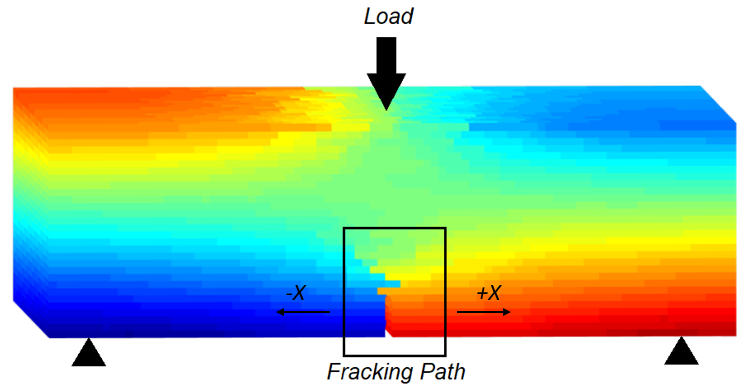
\includegraphics[width=1\textwidth]{figures/Amir_ME1_LEM_Displacement_Crystalline.png}
\caption{The node displacements in X-axis during the fracking process under the applied bending load}
\label{fig:Amir_ME1_LEM_Displacement_Crystalline}
\end{figure}

The article by Tarokh et al. also reports measurements of acoustic emissions, which serve to localize inter-granular micro-cracks. In the DEM method this could be 
reproduced by using the event of tensile contact failures to call a FISH function which writes the location of that contact into a file. The result, the red dots in 
figure \ref{fig:ME1-dem-ae}, agrees very well with the experimental result for the process zone (dashed rectangle).

\begin{figure}[!ht]
\centering
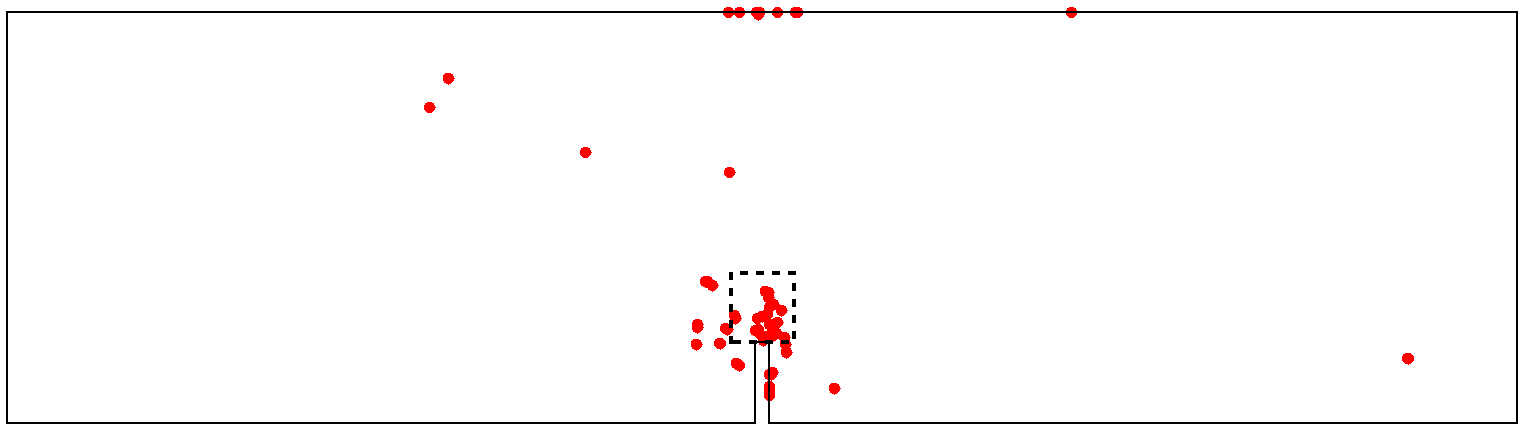
\includegraphics[width=1\textwidth]{figures/sample1-ae-tillmax-v2}
\caption{Locations of acoustic emissions (DEM)}
\label{fig:ME1-dem-ae}
\end{figure}


\clearpage
%\section{Model Exercise 0-1b (01): Bending fracture test (OPA)}
\label{sec:mex01b}
\Authors{Amir Sattari, Keita Yoshioka}

\subsection{Experimental set-up and results}

In this model exercise, the effect of the anisotropy on the fracture toughness of the Opalinus claystones experimentally and numerically is investigated. The description of the experimental setup and the test procedure is explained in section \ref{sec:Fracture_Toughness_Exp}, where a fracture toughness test on a sample with the dimension of 140x30x30 $(mm)$ $(LxWXT)$ is carried out. The notch dimension is 2x10x30 $(mm)$ $(LxWXT)$ and the span length is 120 $mm$. The anisotropy of a claystone depends mainly on the orientation of the embedded layers. When the loading direction is perpendicular ($\bot$) to the layering orientation the materials strength is highest. In contrast, when the loading direction is parallel ($\parallel$) to the layering orientation, the materials strength is the lowest. The peak load attained from the experimental data ($\bot$) is 598 $N$ and the bending stiffness is around 3.3 $GPa$ (Figure \ref{fig:Amir_Fracture_Toughness_Result_20}). The crack mouth opening before the failure is 24 $\mu m$. The 4K video with the 30fps is used to track the reference points on the claystone. Afterward, the image analyzing technique is implemented to determine the CMOD. The 30fps video was not able to detect the brittle failure of the sample and therefore in the experimental data, the post failure response is not well represented. The measured fracture toughness ($\bot$) is $0.746\ MPa.\sqrt\ m$. The anisotropy effect of claystone is observed based on the fracking pattern of different samples under mechanical loading without temperature and humidity control (Figure \ref{fig:Amir_Fracture_Toughness_Fracture_a}). The propagation of fracks parallel to the layering orientation, where the sample is weakest, is observed (Figure \ref{fig:Amir_Fracture_Toughness_Fracture_b}). Similarly, inside the climate chamber, and under 50 and 80 $^{\circ}C$ temperature conditions, the fracture toughness of the claystone is measured ( Table \ref{table:Amir_Fracture_Toughness_Table1}).

\begin{figure}[!ht]
\centering
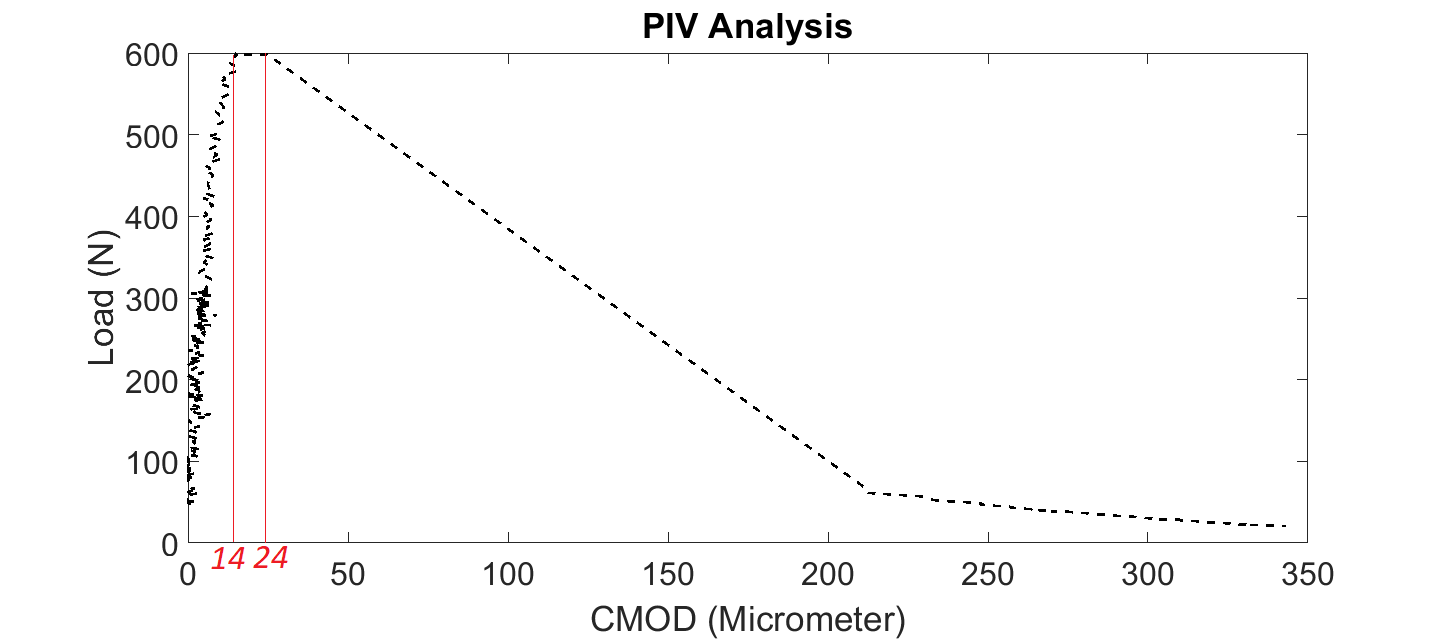
\includegraphics[width=11cm,height=5cm]{figures/Amir_Fracture_Toughness_Result_20.png}
\caption{The load vs. CMOD for the Opalinus claystone sample under the room temperature}
\label{fig:Amir_Fracture_Toughness_Result_20}
\end{figure}

\begin{figure}[!ht]
\centering
\begin{subfigure}[c]{0.43\textwidth}
\centering
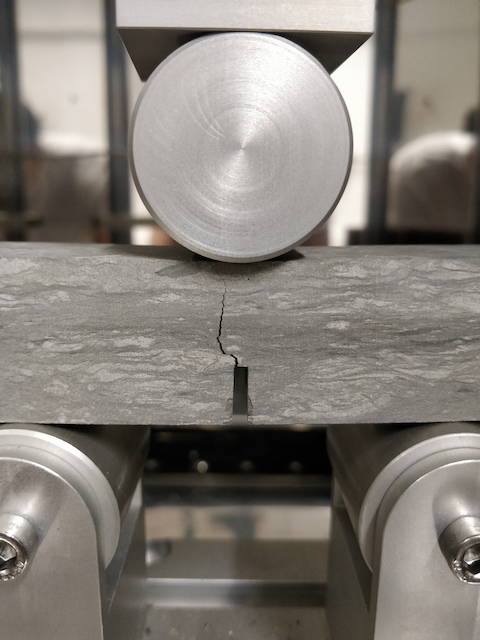
\includegraphics[width=4cm,height=5cm]{figures/Amir_Fracture_Toughness_Fracture_a.png}
\subcaption{}
\label{fig:Amir_Fracture_Toughness_Fracture_a}
\end{subfigure}
\hfill
\begin{subfigure}[c]{0.55\textwidth}
\centering
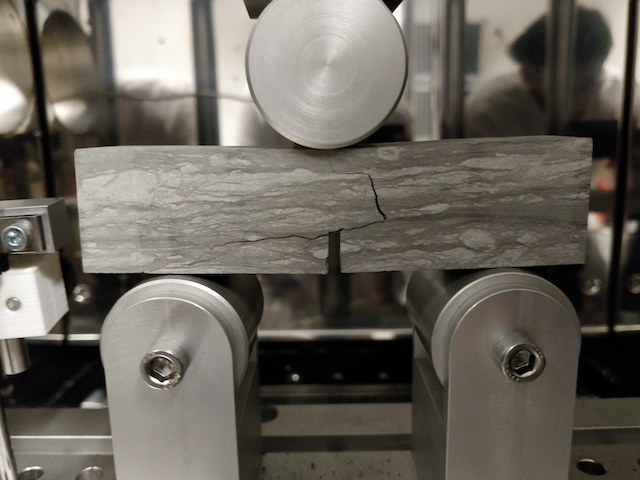
\includegraphics[width=6cm,height=5cm]{figures/Amir_Fracture_Toughness_Fracture_b.png}
\subcaption{}
\label{fig:Amir_Fracture_Toughness_Fracture_b}
\end{subfigure}
\caption{The anisotropy of the frack propagation in claystone (a) the frack propagation parallel to the loading direction, (b) the frack propagation through the weak interface}
\end{figure}

\begin{table}[!ht]
\centering
\begin{center}
\begin{tabular}{ | >{\centering\arraybackslash}X m{14em} | >{\centering\arraybackslash}X m{5em}| >{\centering\arraybackslash}X m{5em} |
>{\centering\arraybackslash}X m{5em} |} 
\hline
Test Results & 20$^{\circ}C$ & 50$^{\circ}C$ & 80$^{\circ}C$ \\
\hline
Peak Force ($N$) & 559 & 482 & 455 \\ 
\hline
Fracture Toughness $MPa.\sqrt m$. & 0.697 & 0.601 & 0.582\\
\hline
\end{tabular}
\end{center}
\caption{The Fracture toughness under different temperature conditions}
\label{table:Amir_Fracture_Toughness_Table1}
\end{table}


\subsection{Model approach}

\subsubsection*{Lattice-Element-Model (LEM)}

The LEM is implemented to investigate the anisotropy of claystone in two cases, where the loading direction is parallel or perpendicular to the layering orientation. The LEM setup ($\bot$) is generated in 2D with the back calculation of the outputs from the fracture toughness \ref{sec:Fracture_Toughness_Exp} and splitting \ref{sec:Brazilian_Disk_Exp} experimental results. The materials strength in perpendicular direction is considered to be 5 times higher than parallel case. The fracture paths for both ($\bot$) and ($\parallel$) cases are shown in Figure \ref{fig:Amir_ME1_LEM_Perpendicular} and \ref{fig:Amir_ME1_LEM_Parallel}, respectively. Figure \ref{fig:Amir_ME1_LEM_Claystone} illustrates the comparison between the experimental and numerical data. As discussed before, the post failure behavior does not match due to the experimental shortage of capturing the true load-displacements.


\begin{figure}[!ht]
\centering
\begin{subfigure}[b]{0.55\textwidth}
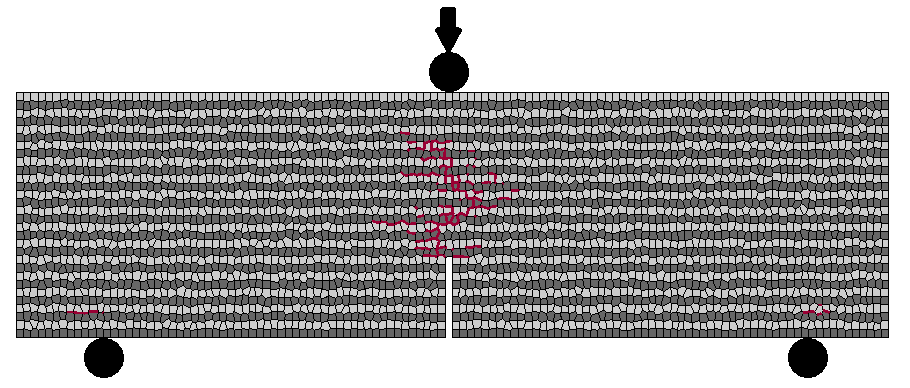
\includegraphics[width=1\linewidth]{figures/Amir_ME1_LEM_Perpendicular.png}
\subcaption{}
\label{fig:Amir_ME1_LEM_Perpendicular}
\end{subfigure}
%\hfill
\begin{subfigure}[b]{0.55\textwidth}
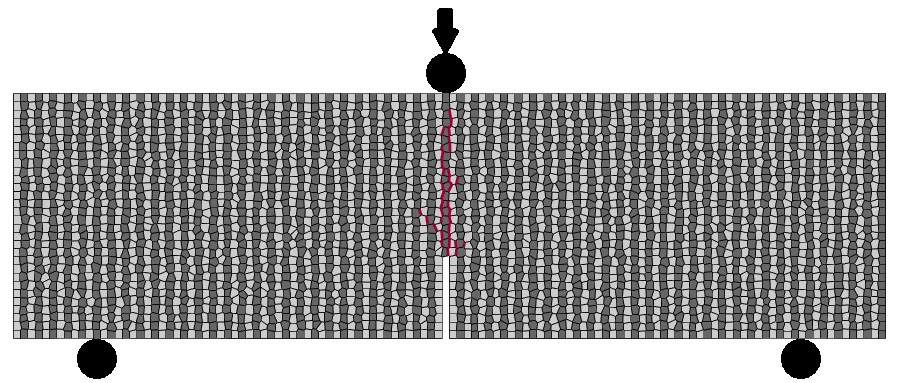
\includegraphics[width=1\linewidth]{figures/Amir_ME1_LEM_Parallel.png}
\subcaption{}
\label{fig:Amir_ME1_LEM_Parallel}
\end{subfigure}
\caption{The fracking path under loading direction (a) perpendicular, and (b) parallel to the layering orientation}
\end{figure}

\begin{figure}[!ht]
\centering
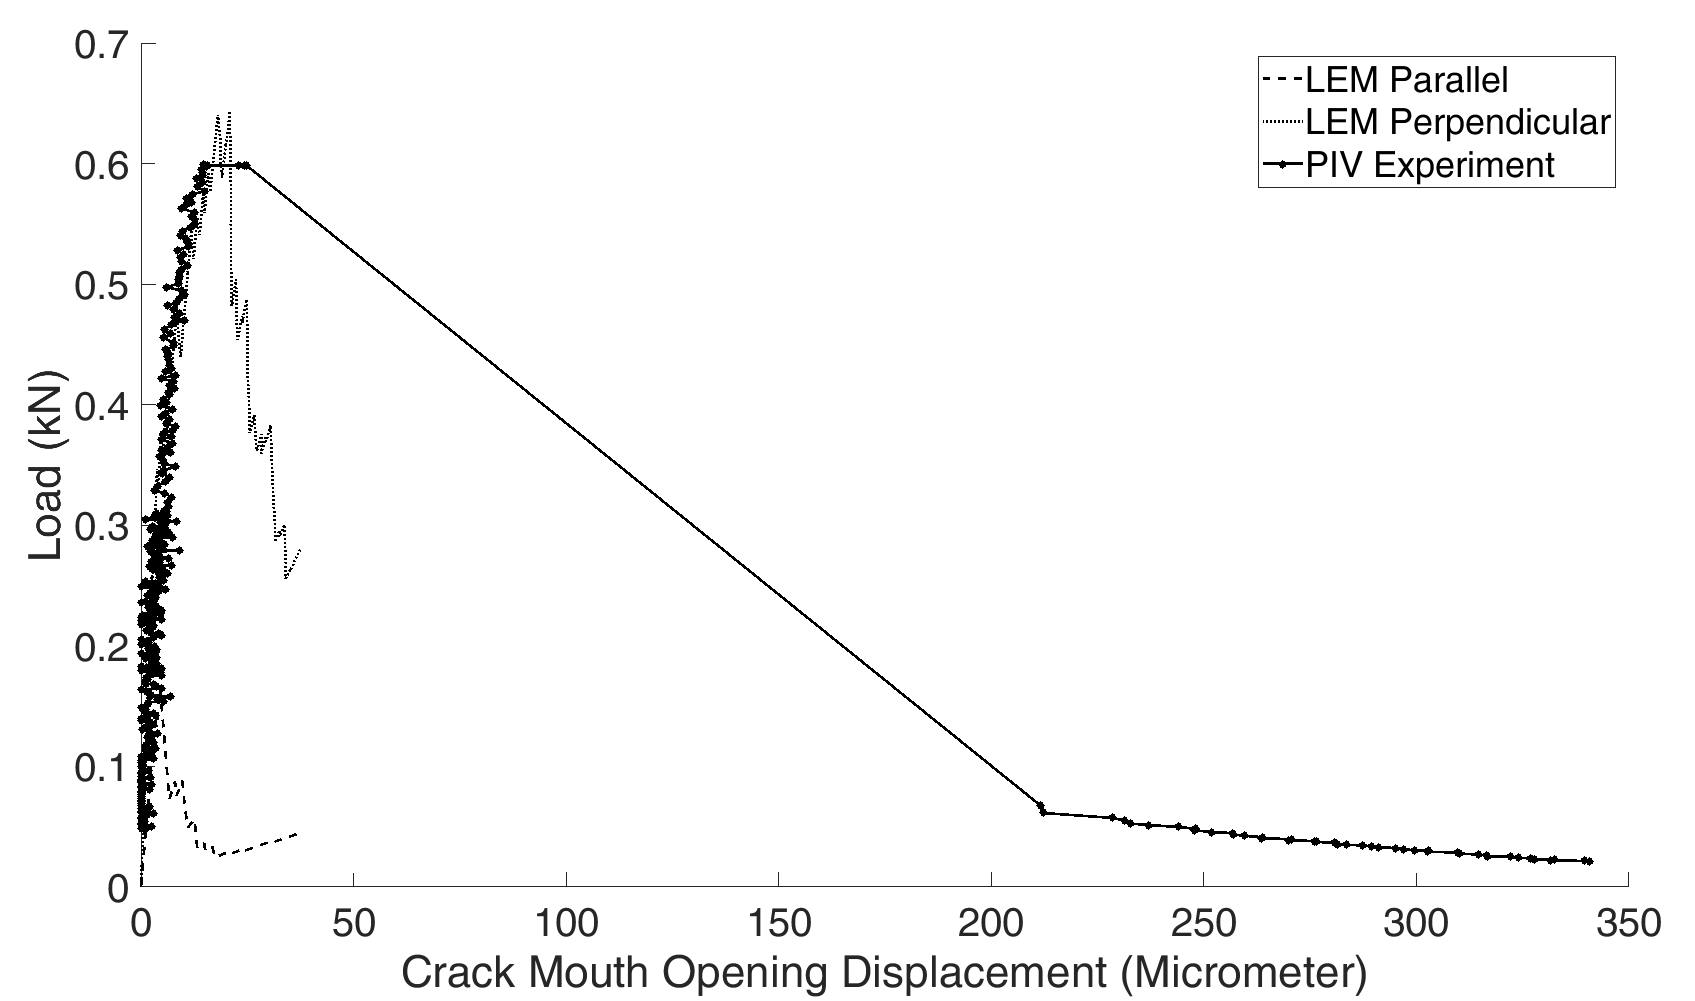
\includegraphics[width=0.75\textwidth]{figures/Amir_ME1_LEM_Claystone.png}
\caption{The comparison of experimental and numerical data for effect of anisotropy in Opalinus claystone} 
\label{fig:Amir_ME1_LEM_Claystone}
\end{figure}

\subsubsection*{Finite-Element-Approach: Variational Phase-Field (VPF)}

The anisotropy claystone sample simulations were also performed with the variational phase-field model.
The material strength contrast in the laminations is realized through a contrast in the fracture toughness. 
For the "weaker" layer, the fracture toughness of 20 $Pa \cdot m$ is assigned while 100 $Pa \cdot m$ is for the "stronger" layer.
Consistently to the LEM simulations, the strength was alternated every 1 $mm$. 
Initial strength set-up for the lamination parallel and orthogonal can be found in Fig.~\ref{fig:ME1_ext_vpf_para_init} and Fig.~\ref{fig:ME1_ext_vpf_orth_init} respectively.
Fracture simulation results are in Figs.~\ref{fig:ME1_ext_vpf_para_result} and~\ref{fig:ME1_ext_vpf_orth_result}, and the force vs. CMOD is in Fig~\ref{fig:ME1_ext_vpf_FvsCMOD}.

\begin{figure}[!ht]
\centering
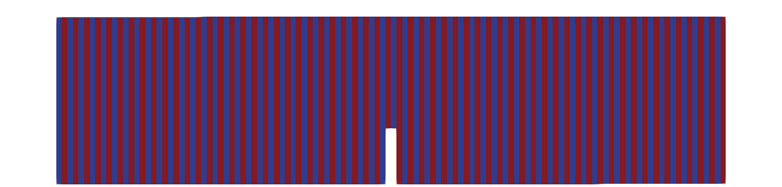
\includegraphics[width=1\textwidth]{figures/ME1_ext_2D_parallel_init.png}
\caption{Sample for parallel to the lamination}
\label{fig:ME1_ext_vpf_para_init}
\end{figure}

\begin{figure}[!ht]
\centering
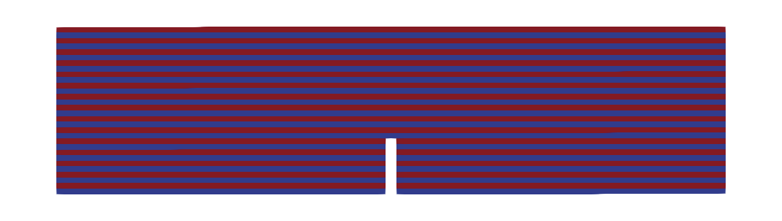
\includegraphics[width=1\textwidth]{figures/ME1_ext_2D_orthogonal_init.png}
\caption{Sample for orthogonal to the lamination}
\label{fig:ME1_ext_vpf_orth_init}
\end{figure}

\begin{figure}[!ht]
\centering

\includegraphics[width=1\textwidth]{figures/ME1_ext_2D_para_result.png}
\caption{Result of parallel to the lamination}
\label{fig:ME1_ext_vpf_para_result}
\end{figure}

\begin{figure}[!ht]
\centering

\includegraphics[width=1\textwidth]{figures/ME1_ext_2D_orth_result.png}
\caption{Result of orthogonal to the lamination}
\label{fig:ME1_ext_vpf_orth_result}
\end{figure}

\begin{figure}[!ht]
\centering
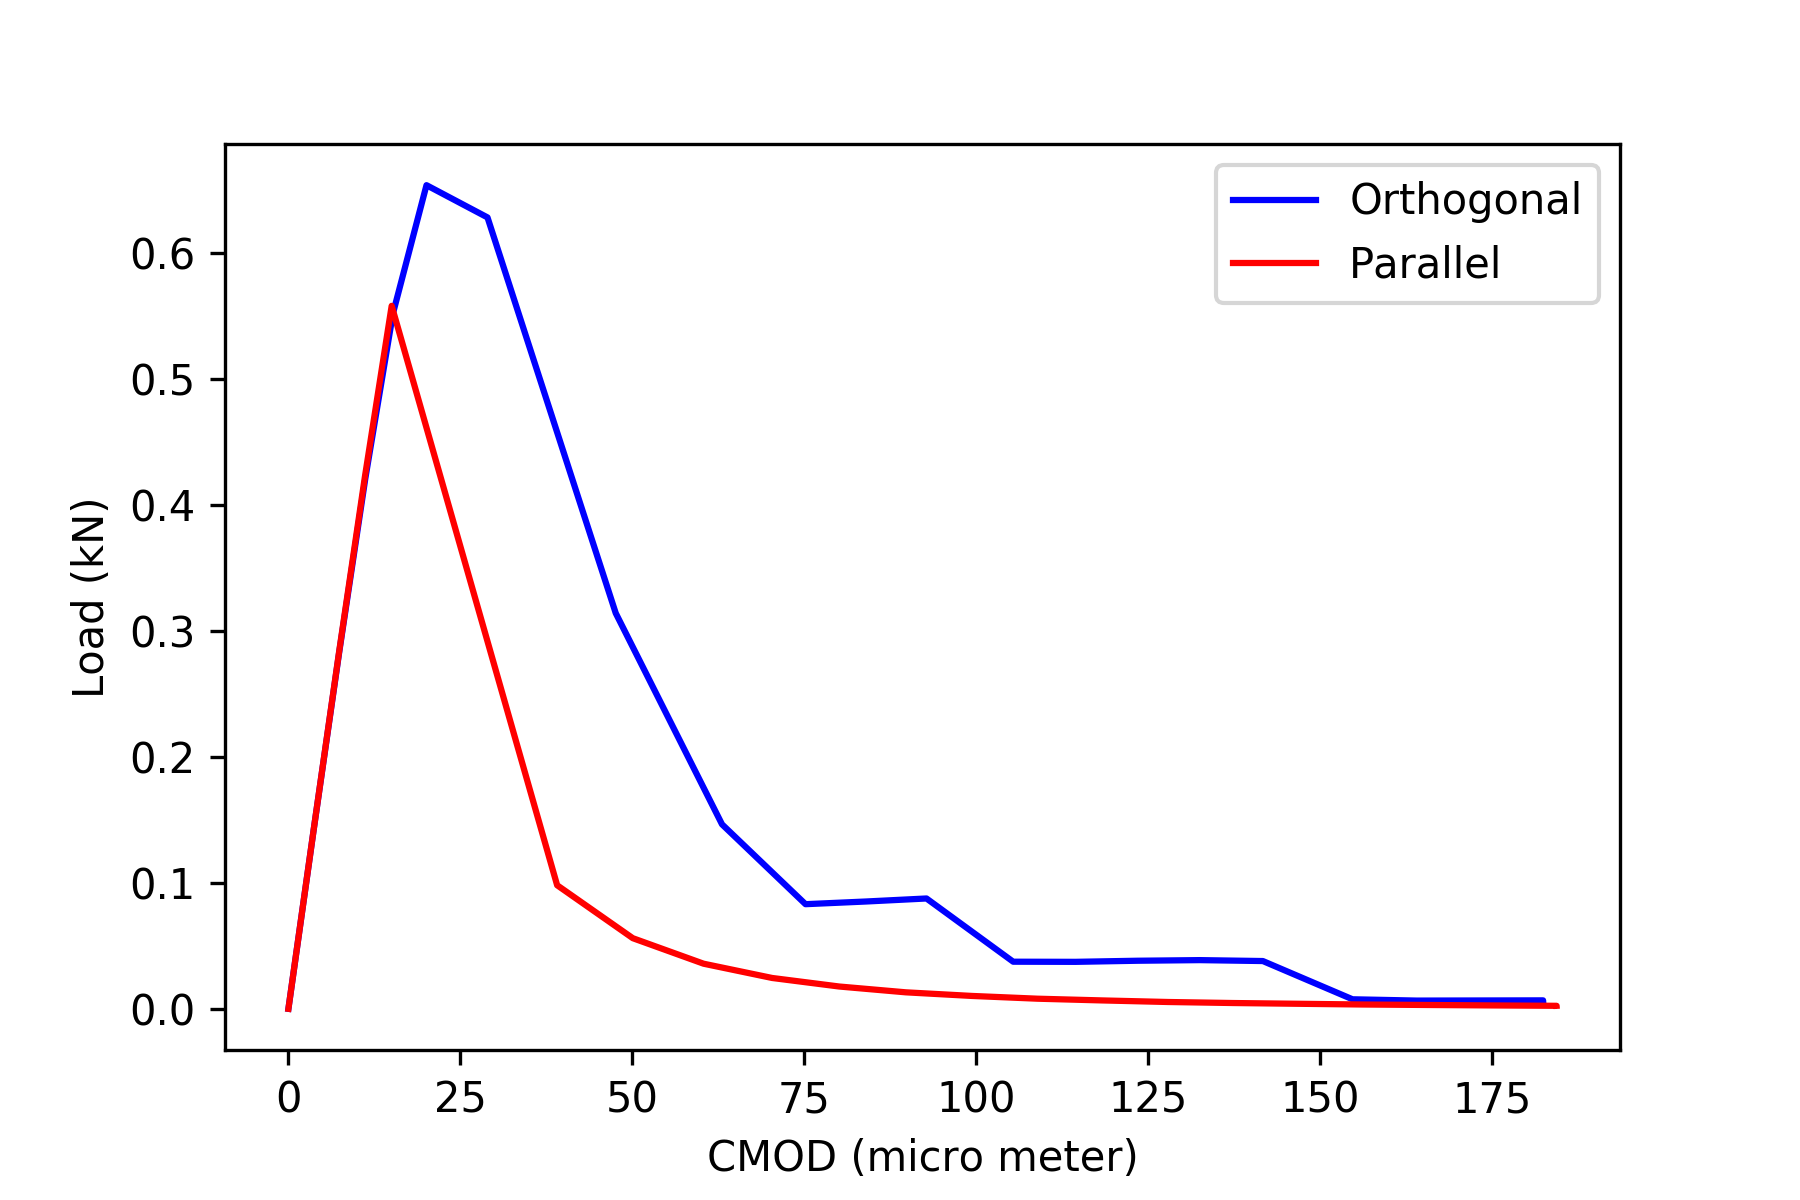
\includegraphics[width=1\textwidth]{figures/VPF_ME1_ex_NF_CMOD.png}
\caption{Force vs. CMOD}
\label{fig:ME1_ext_vpf_FvsCMOD}
\end{figure}

\subsubsection{Results and discussion}

The lattice model is able to capture the existing anisotropy in the Opalinus claystone material. The fracking path dependence on the orientation of the embedded layers is shown in Figure \ref{fig:Amir_ME1_LEM_Perpendicular} and \ref{fig:Amir_ME1_LEM_Parallel}, which matches the experimental data given in Figure \ref{fig:Amir_Fracture_Toughness_Fracture_b}. Due to the layering orientation and stress distributions (in $\bot$ case), the fracking path has zigzag pattern following the weakest interface bonds. This irregularity of the frack path is not captured in VPF model. As mentioned before, the post failure results do not match experimental data due to the experimental tests limitation. The lattice model is validated with the experimental data exist for the ($\bot$) case and is extended to model the ($\parallel$) case, where the loading direction is parallel to the embedded layers. According to the Figure \ref{fig:Amir_Fracture_Toughness_Fracture_a}, the frack path is a straight line through the weak interface bond. More investigation needs to be done to determine and investigate the Opalinus claystone fracture toughness under different loading to the embedded layers orientation and the effect of the humidity and temperature on the fracture toughness. 
%Additionally, the quantitative comparison of the results both for lattice and VPF models should be carried out.
The simulations by V-pf show similar trends observed in the lattice model.
For the lamination parallel case ($\parallel$), the crack is nucleated at a lamination with the lower fracture toughness and propagated straight through.
The force response is also brittle and it declined very quickly after the failure.
The lamination orthogonal case ($\bot$) shows more step--wise crack growth (Fig~\ref{fig:ME1_ext_vpf_para_result}. 
After the nucleation, it repeatedly stopped at the interfaces before the strong lamination and propagated through the weak lamination with ease (Fig~\ref{fig:ME1_ext_vpf_orth_result}.
The force vs. CMOD curve (Fig~\ref{fig:ME1_ext_vpf_FvsCMOD} also exhibits the non--smooth crack propagation response of the lamination orthogonal case. 

\clearpage
%------------------------------------------------------------------------------
%\section[MEX 0-2: Humidity controlled long-term bending test]{Model-Experiment-Exercise MEX 0-2:\\Humidity controlled long-term bending test}
\label{sec:mex13}
%------------------------------------------------------------------------------
\Authors{Thomas Nagel}
%------------------------------------------------------------------------------
%------------------------------------------------------------------------------
\subsection{Experimental set-up}
%------------------------------------------------------------------------------
\begin{wrapfigure}{l}{8cm}
\centering
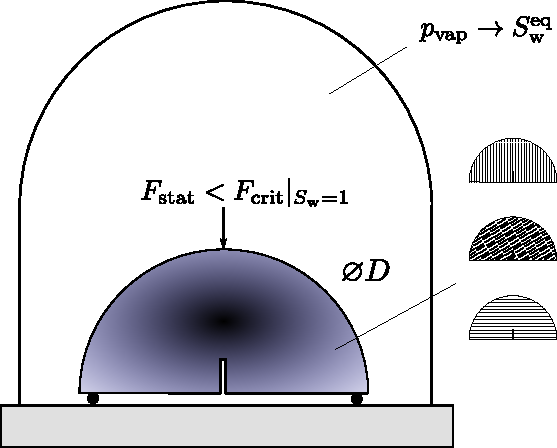
\includegraphics[width=8cm]{figures/GeomInt_MEx13.pdf}
\caption{Concept for a humidity controlled long-term bending test setup}
\label{fig:GeomInt_MEx13}
\end{wrapfigure}
The background for this proposal is the CD-A experiment in Mt. Terri in which cyclic humidity variations cause measurable fluctuations in the crack mouth opening. However, it is less well known whether this leads to crack closure or progressive crack growth. 

From a modelling perspective, the intention is to investigate more deeply several coupling effects in a H\textsuperscript{2}M setting. Thus, the focus is on Experiment B in the description below. Therefore, the test is defined as follows:

\begin{itemize}
	\item Three-point bending tests are performed on semi-cylindrical samples. the reason for the sample shape is simply an easier sample preparation compared to rectangular prismatic bars.
	\item In principle, anisotropy can be studied by using cores from appropriately aligned bore holes. Standard tests would allow studying orientation-dependent fracture toughness etc. (\textbf{Experiment A})
	\item The CMOD and the displacement of the load point should be measured. If possible, the full displacement field on the sample's face can be measured by optical methods.
	\item For \textbf{Experiment B}, the same setup is used but the samples are put into a desiccator (or other humidity-controlled environment).
	\item A static load (dead weight) is applied to a fully saturated sample which is \textit{sub-critical}, i.e. this load does not lead to immediate failure. If rate-dependent effects (creep) can be considered irrelevant, failure of the sample will not occur over time. This should be checked by maintaining one control sample at full saturation throughout by choosing the appropriate humidity in the chamber. If that breaks after a given time, the time-to-failure becomes another comparison metric.
	\item Subsequently (other samples), the humidity is decreased to a low value in order to initiate sample desaturation. An inhomogeneous saturation field will result.
	\item Cyclic effects, such as in the in-situ experiment, will not be considered here.
\end{itemize} 

%------------------------------------------------------------------------------
\subsection{Model approach}
%------------------------------------------------------------------------------

With the saturated sample serving as a reference for potential sub-critical crack growth, the models can now be used to shed light onto the relative relevance of the following phenomena:
\begin{itemize}
	\item Desaturation causes shrinkage of the clay. Due to the desaturation front progressing from the sample's surface, tensile stresses will develop in the superficial zone of the sample depending on the drying rate. These may elevate local loads in the crack tip or even act as additional stress concentrators at the crack tip. Hence, desaturation may drive the sample to failure.
	\item A competing mechanism is brought about by the suction-induced strengthening. Desaturation is associated with the build-up of significant capillary pressures which act as suction stresses and increase the effective confinement, thus increasing strength. Thus, desaturation may via this mechanism act in a stabilizing manner. In that case, failure would not occur and the experimental task would be to observe whether $F_\text{crit}$ increases with desaturation; thus, the sample would have to be loaded to failure. An extension of the test could entail loading each sample to failure after the desaturation experiment has finished, if it hasn't already failed.
\end{itemize}

\clearpage
%------------------------------------------------------------------------------
\section*{WP1: Pathways through swelling/shrinking processes (clay rock)}
%------------------------------------------------------------------------------
%\section{Model Exercise 1-1 (05): Swelling of clay}
\label{sec:mex05}
%------------------------------------------------------------------------------
\Authors{Amir Sattari, Keita Yoshioka, Mattias Nest}
%------------------------------------------------------------------------------
Model Exercise (MEX 1-1) investigates the swelling characteristics of the sandy Opalinus claystone. The numerical and experimental approaches are considered to understand the governing factors, which result in materials behavior change, during the swelling process. 


\subsection{Experimental set-up}

\todo[inline]{[IfG](MN) small description of the experimental procedure and the results }

%------------------------------------------------------------------------------


%------------------------------------------------------------------------------
\subsection{Model approach}
\subsubsection*{Lattice element model}

With the application of the lattice model, the simulation of the swelling process in Opalinus Claystone sample is investigated. The experimental data provided by IfG Leipzig are used to determine the heave, swelling pressure and the change of permeability. The expansion of the elements based on the shrinkage and swelling model described in section \ref{Section:ShrinkageLattice} is carried out. The expansion of the elements results in decrease of the hydraulic aperture and therefore lower permeability values. However, during the swelling process the micro fracking is also observed. The elements expansion lead to higher axial confinement stresses between the Voronoi cells, which is represented by interface elements. The linear strains parallel and perpendicular to the embedded layers found in section \ref{sec:mex06} are used to determine the swelling coefficient values. Eventually, the outcome of the simulation is compared to the experimental results. 

\todo[inline]{[CAU] Please add LEM results}

\todo[inline]{Amir: Keita Will you participate in this MEX?}

%------------------------------------------------------------------------------
\subsection{Results and discussion}
\clearpage
\clearpage
%------------------------------------------------------------------------------
%\section{Model Exercise 1-2 (06): The drying and wetting paths of Opalinus Claystone}
\label{sec:mex06}
%------------------------------------------------------------------------------
\Authors{Amir Shoarian Sattari, Keita Yoshioka}
%------------------------------------------------------------------------------

The simulation of the drying and wetting processes and evolution of the micro pathways in Opalinus claystone are the focus of the this model exercise (MEX 1-2). In this matter, the experimental data are used to model the shrinkage and swelling processes. Additionally, the change of hydraulic conductivity both in parallel and perpendicular to the embedded layering orientations is investigated. It is shown that due to the inherent anisotropy of claystone material, the materials behavior in parallel and perpendicular orientations are different.  

%------------------------------------------------------------------------------
\subsection{Experimental set-up}
%------------------------------------------------------------------------------
The prepared two cylindrical thin sections of sandy Opalinus claystone (Fig. \ref{fig:Amir_Shrinkage_Full_Setup}) are used to determine the drying and wetting paths. The saturated salt solutions are used to apply different osmotic suctions. The considered salt solution and its induced suction and relative humidity values in the constant room temperature of 20 $^{\circ}C$ are listed in Table \ref{table:Amir_Shrinkage_SaltSolutions}. The suction values range from 3.2 up to 367 $MPa$, which insures both drying and wetting paths. The fluctuation of the temperature is negligible. The first sample is used to determine the linear axial strains (Fig. \ref{fig:Amir_Shrinkage_Sensors}) along the embedded layers, which are arranged in a parallel and perpendicular orientations. The second sample is used to determine the water content change during the wetting and drying paths.

\begin{figure}[!ht]
\begin{subfigure}[c]{0.48\textwidth}
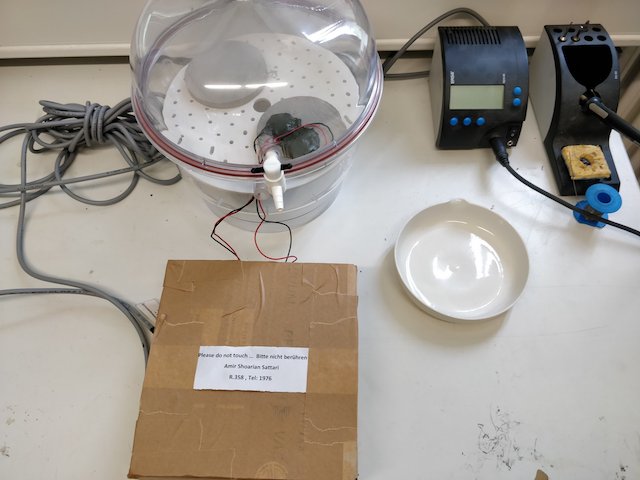
\includegraphics[width=1\textwidth]{figures/Amir_Shrinkage_Full_Setup.png}
\subcaption{}
\label{fig:Amir_Shrinkage_Full_Setup}
\end{subfigure}
\hfill
\begin{subfigure}[c]{0.48\textwidth}
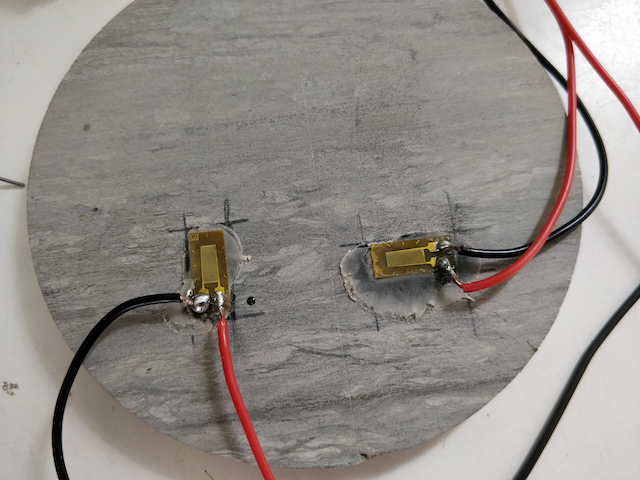
\includegraphics[width=1\textwidth]{figures/Amir_Shrinkage_Sensors.png}
\subcaption{}
\label{fig:Amir_Shrinkage_Sensors}
\end{subfigure}
\caption{The (a) desiccator setup, and (b) arraignment of the strain gauge strips on Opalinus claystone surface}
\end{figure}

The considered salt solution and its induced suction and relative humidity values in the constant room temperature of 20 $^{\circ}C$ are listed in Table \ref{table:Amir_Shrinkage_SaltSolutions}.

\begin{table}[h!]
\centering
\begin{center}
\begin{tabular}{ |>{\centering\arraybackslash}X m{7em}|>{\centering\arraybackslash}X m{10 em}|>{\centering\arraybackslash}X m{7em}|} 
\hline
Salt Solution & Relative Humidity (\%) & Suction ($MPa$) \\
\hline
$K_2SO_4$ & 97.6 & 3.2 \\
\hline
$KNO_3$ & 94.6 & 7.5 \\
\hline
$KCl$ & 85.1 & 21.8 \\
\hline
$NaCl$ & 75.5 & 38\\
\hline
$Mg(NO_3)_2$ & 54 & 84 \\
\hline
$MgCl_2$ & 33.1 & 149.5 \\
\hline
$LiCl$ & 12 & 286.7\\
\hline
$LiBr$ & 6.6 & 367.5\\
\hline
\end{tabular}
\end{center}
\caption{The saturated salt solutions relative humidity and suction values at 20 $^{\circ}C$}
\label{table:Amir_Shrinkage_SaltSolutions}
\end{table}

The samples dimension is 100x10 $mm$ $(DxH)$. The equilibrium inside the desiccator is reached when the change of the samples water content is equal to zero. Fig. \ref{fig:Amir_ME6_Strain} depicts the change of suction and axial linear strains in parallel and perpendicular directions. Similarly, Fig.\ref{fig:Amir_ME6_Water} shows the change of water content with applied suction using salt solutions. In drying path, the results indicate a higher strains for a strain perpendicular to the embedded layers. When the suction is higher than 150 $MPa$, the strains in perpendicular direction are almost 4.5 larger than parallel ones. Interestingly, in the wetting path, the differences between the strain gauges are much less. According to the water content data, the air-entry pressure for a sandy Opalinus claystone is around 25 $MPa$.

\begin{figure}[!ht]
\begin{subfigure}[b]{1\textwidth}
\centering
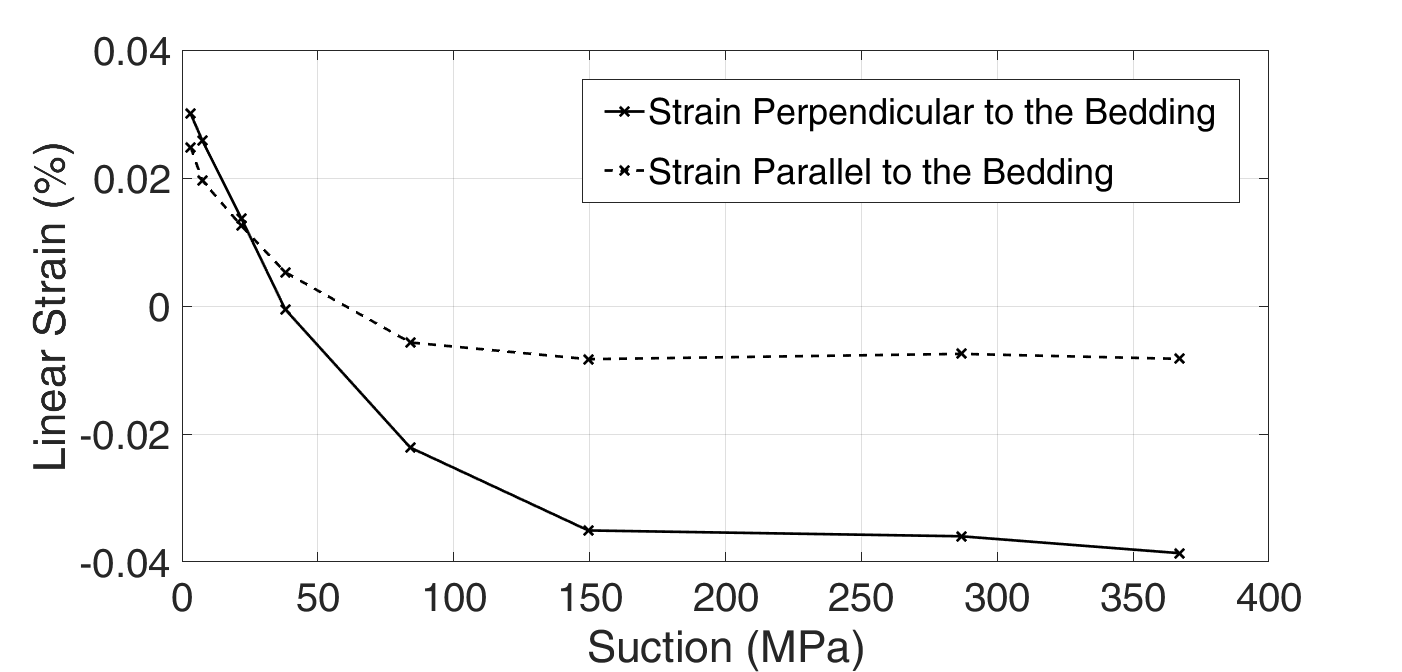
\includegraphics[width=11cm,height=6cm]{figures/Amir_ME6_Strain.png}
\subcaption{}
\label{fig:Amir_ME6_Strain}
\end{subfigure}
\\
\begin{subfigure}[b]{1\textwidth}
\centering
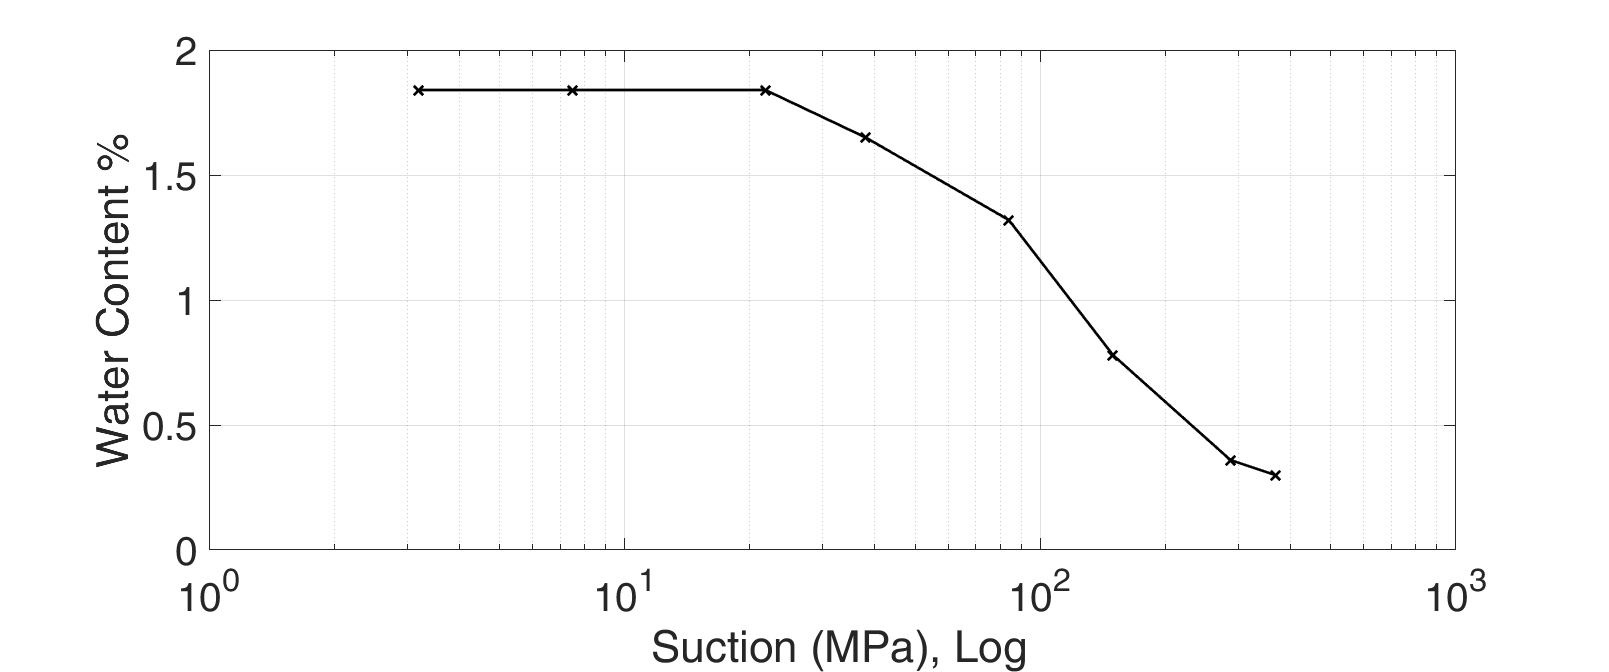
\includegraphics[width=11cm,height=6cm]{figures/Amir_ME6_Water.png}
\subcaption{}
\label{fig:Amir_ME6_Water}
\end{subfigure}
\caption{The drying and wetting paths for Opalinus claystone (a) the suction vs. linear strains, and (b) the suction vs. the water content}
\end{figure}


%------------------------------------------------------------------------------
\subsection{Model approaches}

The simulation results from both of the model methods, lattice element method (LEM) and variational phase field model (VPF) are described and the accuracy of numerical results for modeling the shrinkage process with change of linear or volumetric strains as well as the change of anisotropic hydraulic conductivity are investigated. 

\subsubsection*{Lattice element model}

With the application of the integrated interface element \cite{Sattarietal2019b} the drying and wetting processes in the Opalinus claystone are simulated. The linear strain of the elements are calculated based on the experimental data. The initial hydraulic conductivity ($k_h$) values are approximated according to the technical Report, Mont Terri 2008-04 as,

\begin{align}
\label{eq:LEM_ME6_1}
\begin{split}
k_{h,\parallel}=2\times{10}{^{-13}}
\quad , \quad
k_{h,\bot}=0.6\times{10}{^{-13}}
\end{split}
\end{align}

While considering the cubic law for flow transfer through the porous medium, the hydraulic aperture or length of the interface element is calculated as,

\begin{align}
\label{eq:LEM_ME6_2}
\begin{split}
a_h=\sqrt{\frac{12k_h\nu_f}{g}}
\quad , \quad
a_{h,\parallel}=4.95\times{10}{^{-10}}
\quad , \quad
a_{h,\bot}=2.71\times{10}{^{-10}}
\end{split}
\end{align}

where $\nu_f=1.004\times{10}{^{-6} [m^2.s^-1]}$ and $g=9.8$. The domain is generated using the vectorizable lattice element with defined layers as described in previous sections (Fig. \ref{fig:Amir_ME6_Lattice_Setup}). The interface length is defined based on Eq. \ref{eq:LEM_ME6_2}. The interface strength between two layers is assumed to be 5 times weaker than the bond between a same layer. Therefore, a fracking along the layers (X and Z direction) is expected, Which results in higher hydraulic conductivity values as the wetting and drying process continues (Fig. \ref{fig:Amir_ME6_Lattice_Frack}). Fig. \ref{fig:Amir_ME6_Lattice_Drying}) depicts the change of hydraulic conductivity along three axis of X, Y and Z. As expected, the change of the hydraulic conductivity during the drying process is the lowest along the Y axis, where the drying process is perpendicular to the embedded layering orientation. 

\begin{figure}[!ht]
\begin{subfigure}[c]{0.5\textwidth}
\centering
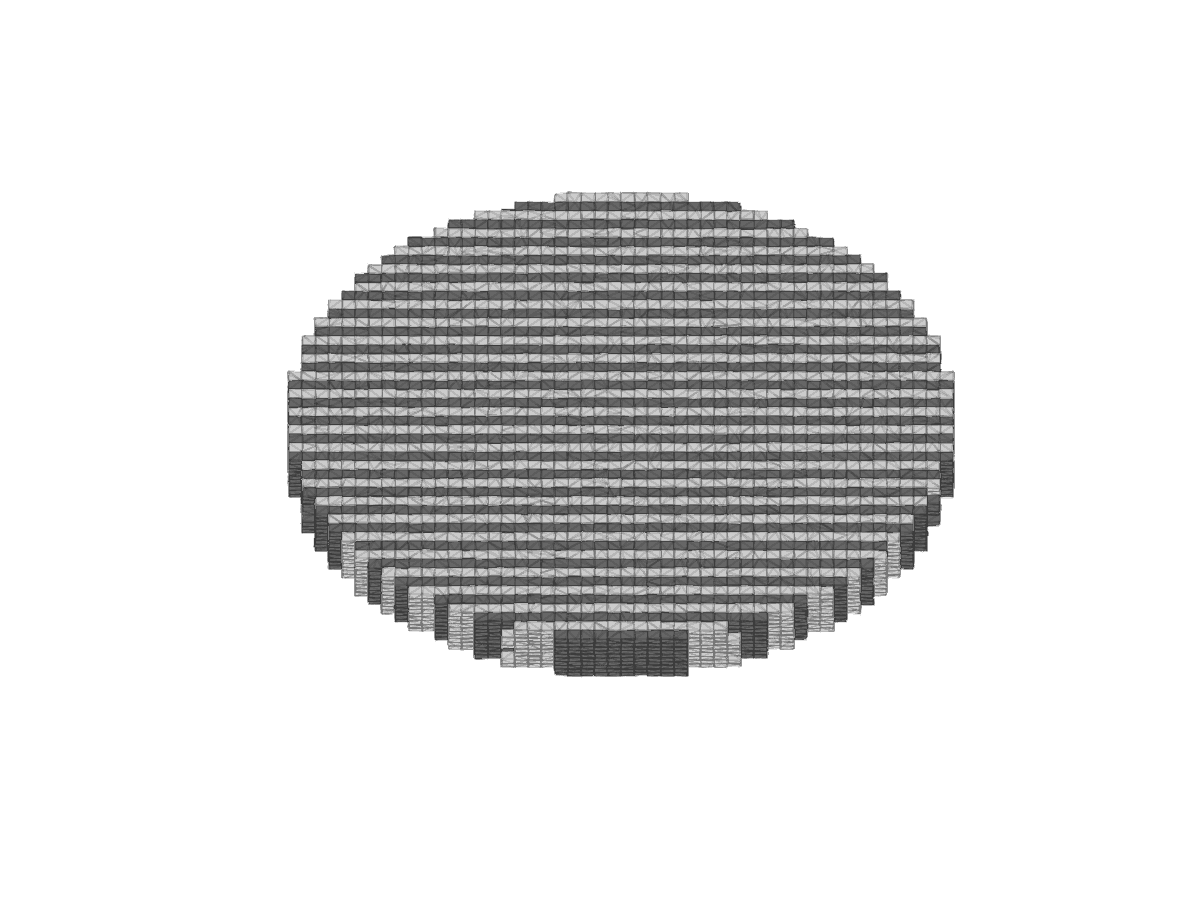
\includegraphics[width=5cm,height=5cm]{figures/Amir_ME6_Lattice_Setup.png}
\subcaption{}
\label{fig:Amir_ME6_Lattice_Setup}
\end{subfigure}
\begin{subfigure}[c]{0.5\textwidth}
\centering
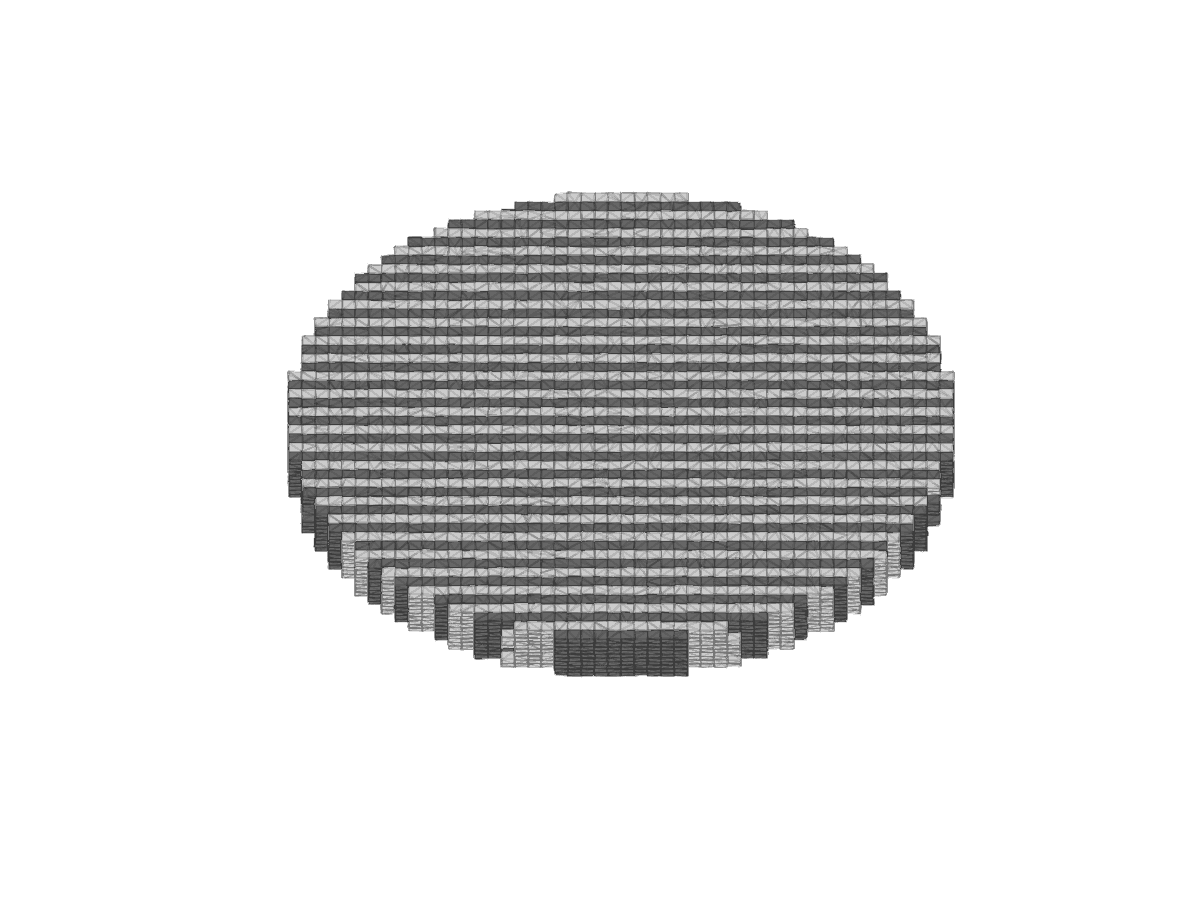
\includegraphics[width=5cm,height=5cm]{figures/Amir_ME6_Lattice_Setup.png}
\subcaption{}
\label{fig:Amir_ME6_Lattice_Frack}
\end{subfigure}
\caption{The (a) generated domain for simulation of the drying and wetting processes, and (b) fracking paths shown with red surfaces}
\end{figure}


\begin{figure}[!ht]
\centering
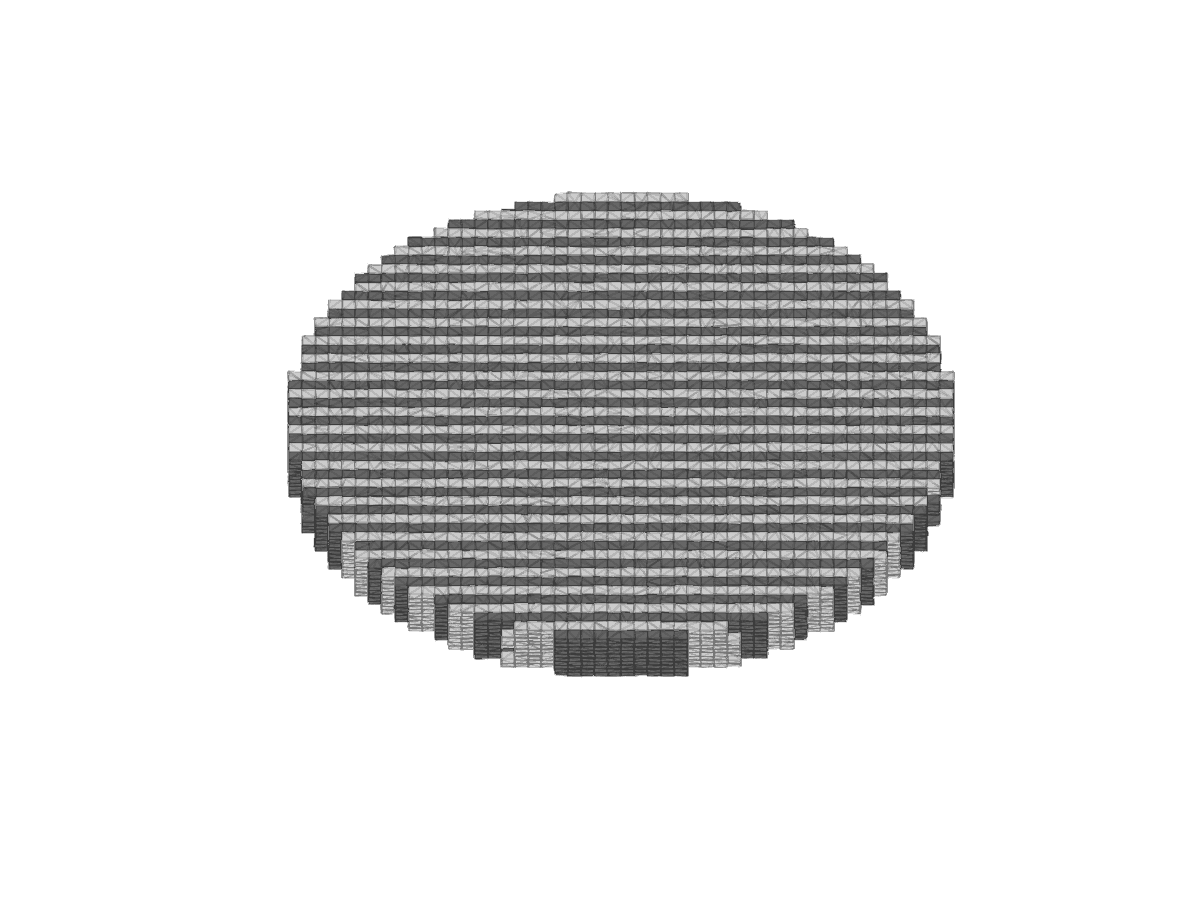
\includegraphics[width=8cm,height=5cm]{figures/Amir_ME6_Lattice_Setup.png}
\caption{The change of hydraulic conductivity along three axis for Opalinus claystone under drying process}
\label{fig:Amir_ME6_Lattice_Drying}
\end{figure} 


%-----------------------------


\subsubsection*{Finite-Element-Method: Variational-Phase-Field (VPF)}
While couplnng of unsaturated flow (Richards flow) and variational phase-field based formulation of fracture mechanics is underway in OGS, the contribution from VPF is being planned. 
Once the model becomes available, strain changes driven by shrinkage or swelling of the sample which is subject to the pore--pressure and the partial saturation changes is modeled utilizing the current Richard--Mechanics implementation in OGS. Then desiccation cracking will be simulated through the variational phase-field using the strain energy contributed from the shrinkage and swelling.
A tentative FEM mesh prepared is shown in~\ref{fig:ME5_VPF_setup}.
The alternating hydraulic conductivities and the material strength will need to be assigned accordingly to the LEM simulation.

\begin{figure}[!ht]
\centering
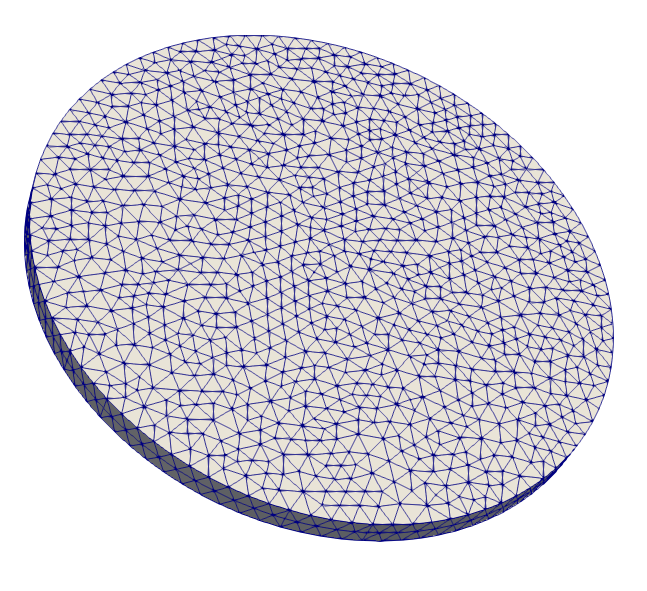
\includegraphics[width=0.75\textwidth]{figures/ME5_VPF_mesh.png}
\caption{The generated FEM mesh for shrinkage process}
\label{fig:ME5_VPF_setup}
\end{figure} 
%------------------------------------------------------------------------------
\subsection{Results and discussion}

The experimental data assessed during the drying and wetting processes confirms the high anisotropy of Opalinus claystone material. Using the saturated salt solutions to apply the osmotic suction, the change of water content as well as the micro deformations along two axis (parallel and perpendicular) are captured and recorded. Higher anisotropy factors during the drying path than in wetting path is observed (Fig. \ref{fig:Amir_ME6_Strain}). The initial water content of the sample was lower than expected in the literature, mainly due to the sample preparation process, where the sample was subjected to the different relative humidity. Fig. \ref{fig:Amir_ME6_Water} shows the air-entry pressure to be around 25 $MPa$. similarly, the residual pressure corresponding to the residual water content is found to be 180 $MPa$ (for more information regarding the soil-water retention curves see \hl{cite Sattarietal2020}. The numerical lattice model to simulate the drying and wetting paths is implemented and with defining the anisotropy, the change of the hydraulic conductivity along different axis is determined. The results show a similar behavior as seen from experimental data. However, more quantitative comparison of the data between experimental and numerical results is required. 
\clearpage
\clearpage
%------------------------------------------------------------------------------
%%%==============================================================================
%  Model exercise Desiccation under in-situ conditions
%  HS, 05/04/2019
%%==============================================================================
\section[MEX 1-3: Desiccation under in-situ conditions]{Model Exercise 1-3: Desiccation under in-situ conditions}
\label{sec:mex12}
\index{desiccation process}
%------------------------------------------------------------------------------
\Authors{Holger Steeb}
%------------------------------------------------------------------------------
We focus on in-situ (image-based) characterization of desiccation processes of sandy-clay samples
under confined conditions. A cylindrical clay core with diameter $D=30$ mm and height 
$H=60$ mm is embedded in a hollow PEEK (Polyether ether ketone) tube. 
The sample is prepared with a drill hole of $d=5$ mm.
Further, the sample is firstly sealed with a Teflon shrink tube. Secondly the gap between the sample and the PEEK tube is filled with an epoxy resin.
Epoxy and PEEK have low X-Ray absorption properties. Through the embedding, radial deformations of the clay sample are preventing. The top and bottom parts of the samples are (hydraulically) sealed with end-caps. The end-caps allow for axial deformations (should we measure them?) occurring during the shrinkage process. The drill hole is ``open''  allowing for water release/uptake.
The prepared sample with in-situ humidity (fully/partially saturation?) is placed in an environmental chamber (Anton Paar, CDT 100, Peltier heated). Temperature and humidity can be controlled (MHG 100 humidity controller, ProUmid). We plan to plug in a small van which allows for controlled humidity convection in the drill hole. 

Drying/desiccation will be image-based characterized within the open XRCT scanner in Stuttgart. We are aiming for a spatial resolution of $30 / 2500$ = 12 $\mu$m / voxel. XRCT scans will be performed for equilibrium states at certain humidity conditions (at ambient temperature of $\Theta = 20^o$ C).

\todo[inline]{[UoS](HS): Adding a figure (experimental set-up/device)?}

\clearpage
%------------------------------------------------------------------------------
%%%==============================================================================
%  Model exercise Numerical computation of CD/LP experiment (Mont Terri)
%  BV, 24/04/2019
%%==============================================================================
\section[MEX 1-4: CD/LP experiment (Mont Terri)]{Model Exercise 1-4:\\CD/LP experiment (Mont Terri)}
\label{sec:mex10}
%------------------------------------------------------------------------------
\Authors{Bernhard Vowinckel, Gesa Ziefle, Jobst Ma\ss mann}
%------------------------------------------------------------------------------
\subsection{Motivation}
%%%%%%%%%%%%%%%%%%%%%%%%%%%%%%%%%%%%%%%%%%%%%%%%%%%%%%%%%%%%%%%%%%%%%%%%%%%%%%%%%%%%%%%%%%%%
Various areas of research like disposal of nuclear radioactive waste, geothermal energy, and carbon capture and storage (CCS) among others deal with coupled hydraulic-mechanical as well as thermal and chemical processes in the underground. Finite element (FE) codes are a well established tool to strengthen the understanding of the related long-term effects. The German Federal Institute for Geosciences and Natural Resources (BGR) has gathered vast experience with the FE code OpenGeoSys (OGS-5 as described in \cite{kolditz2012})  to compute coupled  hydraulic-mechanical processes for example in the  Mont Terri Rock Laboratory (RL) in Switzerland. Within the project GeomInt (Geomechanical integrity of host and barrier rocks), the focus is on the investigation of the development of discontinuities such as cracks and fissures in claystone, crystalline and rock salt. The Helmholtz Centre for Environmental Research (UFZ) is developing an enhanced version of the FE code OGS-6 (as described in \cite{Naumov:2018}) which has an additional focus on the investigation of these effects.   The present report summarizes the results of a comparison between two simulations of the seasonally induced hydraulic desiccation carried out using OGS-5 (version from November 13th, 2017) and OGS-6 (version from December 7th, 2018), respectively. The comparison focuses on the implementation of the two model approaches: 1) Unsaturated one phase flow, based on the Richards approximation \cite{richards1931} (”Richards Flow”, RF) and 2) poro-elasticity coupled with Richards Flow following \cite{biot1941} (”Richards Mechanics”, RM). These models serve as a basis to extend OGS-6 further towards the dynamics of discontinuities.
\index{Richards mechanics}

%%%%%%%%%%%%%%%%%%%%%%%%%%%%%%%%%%%%%%%%%%%%%%%%%%%%%%%%%%%%%%%%%%%%%%%%%%%%%%%%%%%%%%%%%%%%
\subsection{Problem statement}
%%%%%%%%%%%%%%%%%%%%%%%%%%%%%%%%%%%%%%%%%%%%%%%%%%%%%%%%%%%%%%%%%%%%%%%%%%%%%%%%%%%%%%%%%%%%
In the present study, we analyze an idealized niche that is located in the anticline of the Opalinus Clay formation of Mont Terri RL and has a width and height of 3.15 m and 3.3 m, respectively. The computational scenario is designed according to \cite{ziefle2018}, who successfully reproduced the coupled hydraulic-mechanical behavior of a niche in the tunnel system of the Mont Terri RL.   A cross-sectional view of the model of the niche is given in Figure \ref{fig:setup}. The clayey rock in the niche is uncovered, so that seasonal changes in humidity cause cyclic desiccation and saturation of the rock. The porous medium is subdivided into two material groups. Far away from the niche ($> 2$ m), the rock is undisturbed and reflects the properties of Opalinus clay (ID 1). Close to the niche, an excavation damaged zone (EDZ) is defined (ID 2). For the present study, two relevant processes can be identified. First, owing to the exposure of the niche to seasonal change in humidity, there will be a saturation/desaturation of the porous rock. This process can be analyzed by considering hydraulic effects (RF) only. Second, the changes in capillary pressure induce a stress redistribution. To analyze this problem, the coupled hydro-mechanical process (RM) needs to be considered.

%%%%%%%%%%%%%%%%%%%%%%%%%%%%%%%%%%%%%%%%%%%%%%%%%%%%%%%%%%%%%%%%%%%%%%%%%%%%%%%%%%%%%%%%%%%%
\subsection{Unsaturated one-phase flow using the Richards approximation ( "Richards Flow", RF)}
\label{sec:RF}
\index{Richards flow}
\subsubsection{Model description}
\label{sec:model_RF}
%%%%%%%%%%%%%%%%%%%%%%%%%%%%%%%%%%%%%%%%%%%%%%%%%%%%%%%%%%%%%%%%%%%%%%%%%%%%%%%%%%%%%%%%%%%%
The model "Richards Flow" (RF) is based on the classical Richards equation for unsaturated conditions in porous media flows \cite{richards1931}, which reads:
\begin{equation}\label{eq:richards}
\phi \rho_f \frac{\partial S}{\partial p_c}\frac{\partial p_c}{\partial t} + \nabla \cdot \left(\rho_f \frac{k_\text{rel}\textbf{k}}{\mu_f}(\nabla p_f-\rho_f \textbf{g})\right)= Q_f \qquad ,
\end{equation}
where $\phi$ is the porosity, $\rho_f$ the fluid density, $S$ the fluid saturation, $p_c$ the capillary pressure, $t$ the time, $k_\text{rel}$ the relative permeability, $\textbf{k}$ the intrinsic permeability, $\mu_f$ the dynamic viscosity of the fluid, $p_f=-p_c$ the fluid pressure, $\textbf{g}$ the vector of gravitational acceleration, and $Q_f$ a source term. Note that this approximation neglects the change of gas pressure. Equation \eqref{eq:richards} is parametrized using the classical van Genuchten approach  \cite{vangenuchten1980} for the capillary pressure
\begin{equation}\label{eq:cap_p}
p_c = \max \left(p_d\left(S_\text{eff}^{-1/m}-1\right)^{1-m};p_{c,max}\right)
\end{equation}
and the relative permeability 
\begin{equation}\label{eq:k_rel}
k_\text{rel}=S_\text{eff}^{1/2}\left[1-\left(1-S_\text{eff}^{1-\beta}\right)^\beta\right]^2 \qquad ,
\end{equation}
respectively, where $p_d$ is the air entry pressure, $m$ and $\beta$ are fitting parameters reflecting the pore size distribution, $p_{c,max}$ is the maximum capillary pressure and 
\begin{equation}
S_\text{eff}=\frac{S-S_r}{S_{max}-S_r}
\end{equation}
is the effective saturation. Here, $S_r$ and $S_\text{max}$ are the residual and maximum fluid saturation, respectively.

Parameters were taken from the simulations carried out by \cite{ziefle2018}:
\begin{tabbing} 
Fluid density 		\hspace{4cm} \= $\rho_f=1000 \text{ kg/m}^3$	\\
Dynamic viscosity 	\>				$\mu_f= 1\cdot 10^{-3} \,  \text{Pa s}$\\
Porosity 			\> 				$\phi=0.16$ 					\\
Air entry pressure	\>				$p_d = 2 \cdot 10^{7} \, \text{Pa}$\\
Maximum capillary pressure \> 		$p_{c,max} = 1 \cdot 10^9 \, \text{Pa}$\\
Parameter for capillary pressure   \>	$m = 0.41176$\\
Parameter for relative permeability\> 	$\beta = 0.5$ \\
Residual fluid saturation \>			$S_r = 0.0$ \\
Maximum fluid saturation \> 			$S_\text{max}=1.0$ \\
Gravitational acceleration \>       $\textbf{g}=(0,0)^T$\\
Source term \>                      $Q_f = 0.0 \, \text{kg} / (\text{m}^3 \text{s})$
\end{tabbing}

The parameters $\phi$, $p_d$, $p_{c,max}$ and $m$ entering \eqref{eq:cap_p} and the values for $\beta$, $S_r$ and $S_\text{max}$ in \eqref{eq:k_rel} were reported for Opalinus Clay shale \cite{xu2013,wild2015}, both of which were experimentally determined at the Mont Terri RL.

Consolidated clayrock typically has a bedding owing to the plate like shape of individual primary clay particles. As a result,  clay rock becomes transverse isotropic. For the RF-process, this yields different permeabilities values perpendicular ($k_\perp$) and parallel ($k_\parallel$) to the bedding plane. In the present study, values were taken from the experimental report of \cite{bock2009}. For the EDZ, the permeability is assumed to be one order of magnitude higher than in the undisturbed rock: 
\begin{tabbing} 
Undisturbed rock (ID1)\hspace{3cm} \= $k_{1,\parallel}=6.8\cdot 10^{-20} \,  \text{m}^2$\\
 								   \> $k_{1,\perp}=1.36 \cdot 10^{-20} \, \text{m}^2$\\
EDZ (ID2)						   \> $k_{2,\parallel}=6.8 \cdot 10^{-19}\, \text{m}^2$\\
          						   \> $k_{2,\perp}=1.36 \cdot 10^{-19}\, \text{m}^2$\\
\end{tabbing}

As mentioned above, the niche is located in the anticline of the Mont Terri RL. Hence, the transverse isotropic permeability needs to be transformed into the laboratory frame that corresponds to the bedding plane of the clay rock using
\begin{equation}\label{eq:permeabilities}
\textbf{R k R}^T = \begin{pmatrix} \cos \gamma & -\sin \gamma \\ \sin \gamma & \cos \gamma \end{pmatrix}
\begin{pmatrix} k_\perp & 0 \\ 0 & k_\parallel \end{pmatrix}
\begin{pmatrix} \cos \gamma & \sin \gamma \\ -\sin \gamma & \cos \gamma \end{pmatrix} \qquad ,
\end{equation}
where $\gamma=-32.96^{\circ}$ is the angle of inclination. This transform yields a local coordinate system that forms an orthogonal basis with the set of vectors $e_1=(0.8391,-0.5440)^T$ and $e_2=(0.5440,0.8391)^T$.

The primary variable entering the Richards equation as an unknown is the fluid pressure in the porous medium. This quantity is directly related to air humidity via the Kelvin equation \cite{bond2013}. The initial and boundary conditions for the simulation were set as follows:
\begin{tabbing}
Initial condition \hspace{2cm} \=	$p_0 = -900 \, \text{Pa}$ \\
Boundary condition 	\>				$p_\infty = -900 \, \text{Pa}$ \\
					\>				$p_t = \frac{1}{2}p_\text{min}\left[\sin\left(2 \pi \left( \frac{t}{T}+ \frac{\phi_0}{360}\right)\right) - 1\right]$ \\
\end{tabbing}
where $p_\infty$ is the pressure at the outer boundary for the undisturbed rock and $p_t$ is the seasonal boundary condition at the walls of the niche that reflects the variation of humidity inside the niche (Figure \ref{fig:bc}). Further, $p_\text{min}$ is the minimum pressure reached for the saturation deficit at dry air conditions, $T=365\text{ d}$ is the duration of one seasonal period and $\phi_0=270^{\circ}$ is the phase shift angle to start the simulations with a 'wet'  boundary at the tunnel walls. For the present simulations, $p_\text{min}$ was set to $2.87 \cdot 10^7$ Pa, which corresponds to $S_\text{eff}=0.65$. The total simulation time is $T_\text{tot}= 20T$. To properly resolve the unsteady boundary condition $p_t$ in time, a temporal discretization of $\Delta t = 21400$ s was used unless specified otherwise. 

\begin{figure}
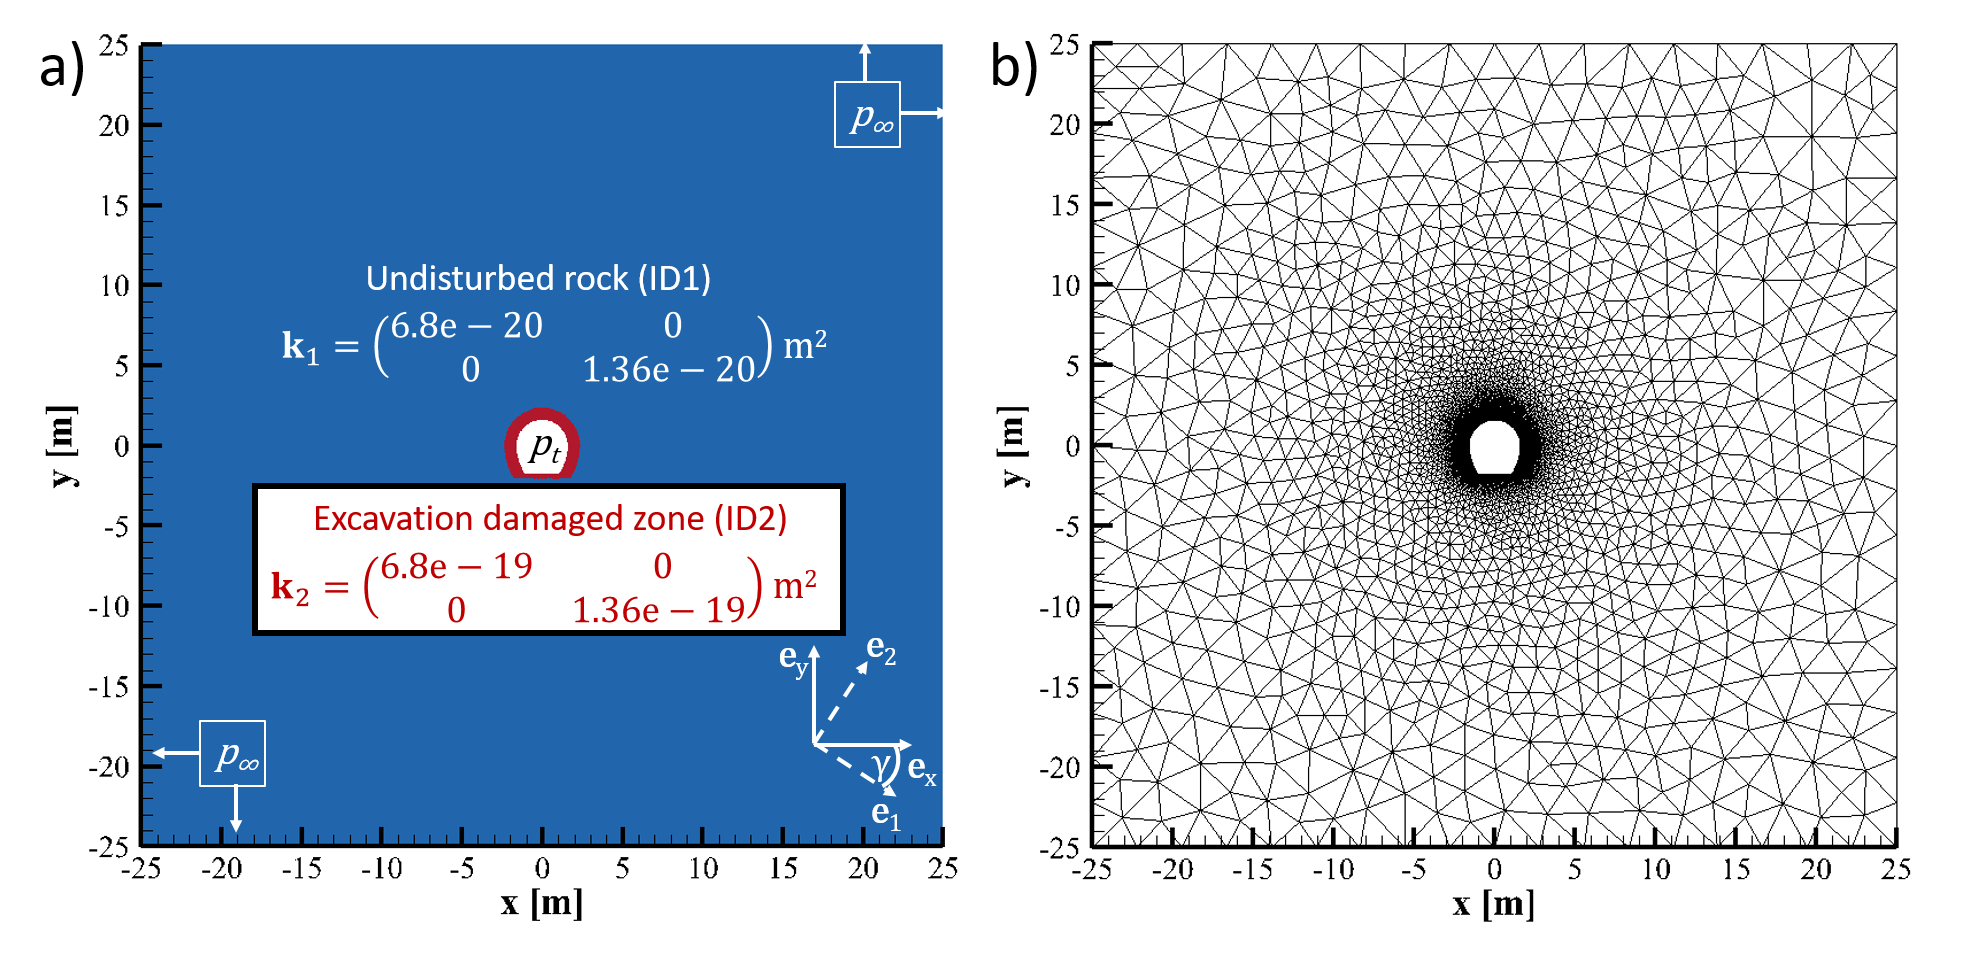
\includegraphics[width=\textwidth, trim=0.4cm 0 0 0, clip]{./figures/MEX10_setup_and_grid.png}
\caption{a) Computational setup and material parameters of the physical problem. b) Triangulated computational grid comprising 5463 nodes. }
\label{fig:setup}
\end{figure}

\begin{figure}
\centering
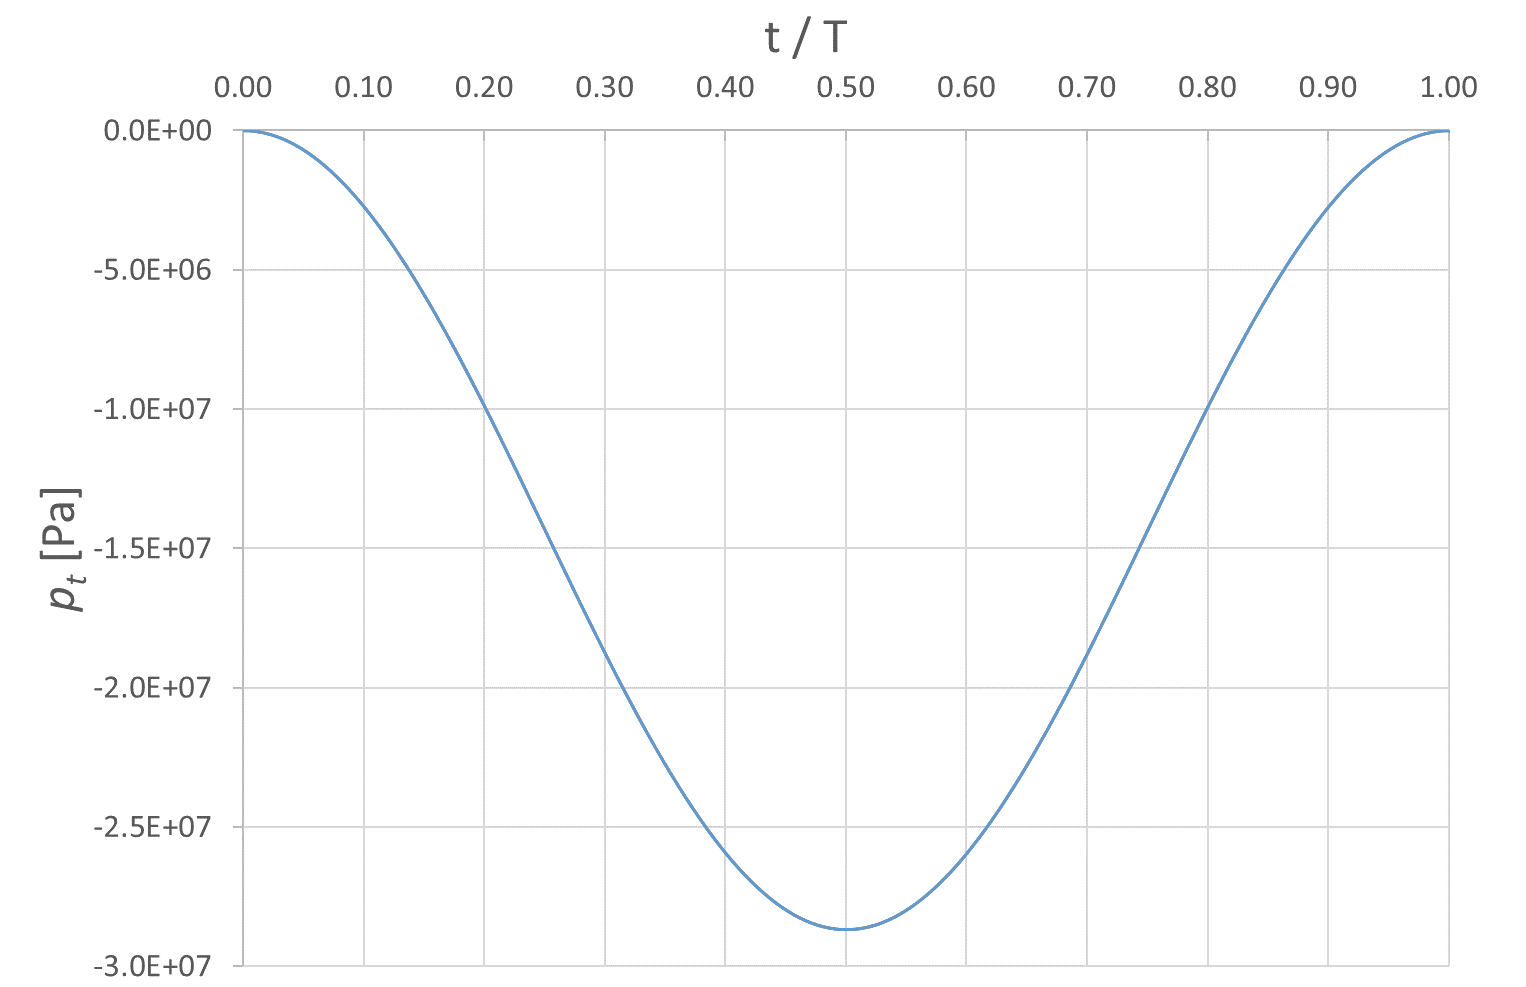
\includegraphics[width=0.7\textwidth]{./figures/MEX10_boundary_condition_tunnel.png}
\caption{Temporal evolution of the dynamic boundary condition at the wall of the niche for one seasonal period $T$. The total simulation time was ${T_\text{tot}=20T}$.}
\label{fig:bc}
\end{figure}

The simulation is set up as a two-dimensional problem. The total extent of the domain is 50 by 50 meters and the domain is discretized by a total of 5463 nodes with elements of triangular shape (Figure \ref{fig:bc}b) unless specified otherwise. This spatial discretization is the exact same mesh as used by \cite{ziefle2018}. A summary of the boundary conditions for the computational domain and the material parameters is given in Figure \ref{fig:setup}a. The seasonal change in pressure boundary conditions at the surface of the niche is shown as a function of time in Figure \ref{fig:bc}. The numerical parameters for the nonlinear and linear solver are listed in Table \ref{tab:solver}.

\begin{table}
 \caption{Numerical parameters of the solvers used in OGS-5 and OGS-6, where $\bf{r}$ and $\bf{b}$ are the residual and the right-hand side vector, respectively, and $\epsilon$ the error tolerance. Further the abbreviations for the solvers and preconditioners mean Conjugate Gradient on the Normal Equations (CGNR), Biconjugate gradient Stabilized Method (BiCGSTAB), and Incomplete LU Factorization Technique (ILUT), respectively.\label{tab:solver}}
\begin{center}
\begin{tabular}{ l | c | c || l | c | c }
\multicolumn{3}{c||}{Nonlinear solver}			 & 	 \multicolumn{3}{ c}{Linear solver} \\
 Parameter 	& OGS-5 		& OGS-6	 & Parameter 			& OGS-5 			& OGS-6	\\
 \hline
 Solver  	 			& Picard 	& Picard & Solver  	 	& CGNR 		& BiCGSTAB \\ 
 Error 	& L2-norm 		& L2-norm  & Error 			& $\Vert\bf{r}\Vert<\epsilon \Vert\bf{b}\Vert$  	& $\Vert\bf{r}\Vert<\epsilon \Vert\bf{b}\Vert$  	\\		
  Error tol. $\epsilon$  	& 1E-5		& 1E-12  & Precon.	& Jacobi		& ILUT\\ 
  Max. iter.			& 50		& 40 	 & Error tol. $\epsilon$		& 1E-12			& 1E-10\\ 
 Relaxation					& 0.0		& n/a	 & Max. iter.	& 20000			& 3000 
\end{tabular}
\end{center}
\end{table}

%%%%%%%%%%%%%%%%%%%%%%%%%%%%%%%%%%%%%%%%%%%%%%%%%%%%%%%%%%%%%%%%%%%%%%%%%%%%%%%%%%%%%%%%%
\subsubsection{Well-developed stage}\label{sec:well_developed}
%%%%%%%%%%%%%%%%%%%%%%%%%%%%%%%%%%%%%%%%%%%%%%%%%%%%%%%%%%%%%%%%%%%%%%%%%%%%%%%%%%%%%%%%%
This well-developed stage is reached after 15 cycles of alternating wet and dry boundary conditions, i.e. 15 years of simulation time. The spatial distribution of $p_f$ and $S_\text{eff}$ is illustrated in Figure \ref{fig:results} for the results generated by OGS-5. Figures \ref{fig:results}a and b show the spatial distribution of the fluid pressure at a dry and a wet phase, respectively. Owing to the variations in pressure $p_t$ at the niche, i.e. relative air humidity inside the gallery,  the rock undergoes cyclic saturation and desaturation. As expected, this affects the saturation at the walls of the niche and in the vicinity of the walls. Farther away  from the boundary, a stable pattern develops for $p_f$ and $S_\text{eff}$ that reflects the transverse isotropic permeabilities prescribed by \eqref{eq:permeabilities}.  Even though the effect of desiccation becomes obvious in concentric ellipses surrounding the niche, the temporal evolution of the boundary condition at the wall of the niche is visible within the EDZ only. At this well-developed stage, the rest of the domain remains unaffected from these changes in $p_t$. The same can be observed for the effective saturation in Figures \ref{fig:results}c and d. Due to the nonlinear dependency of $S_\text{eff}$ and $p_f$ in \eqref{eq:cap_p}, the area that is substantially influenced by the seasonal variation of $p_t$ is even smaller in figures \ref{fig:results}c and d compared to figures \ref{fig:results}a and b.
%
\begin{figure}[t]
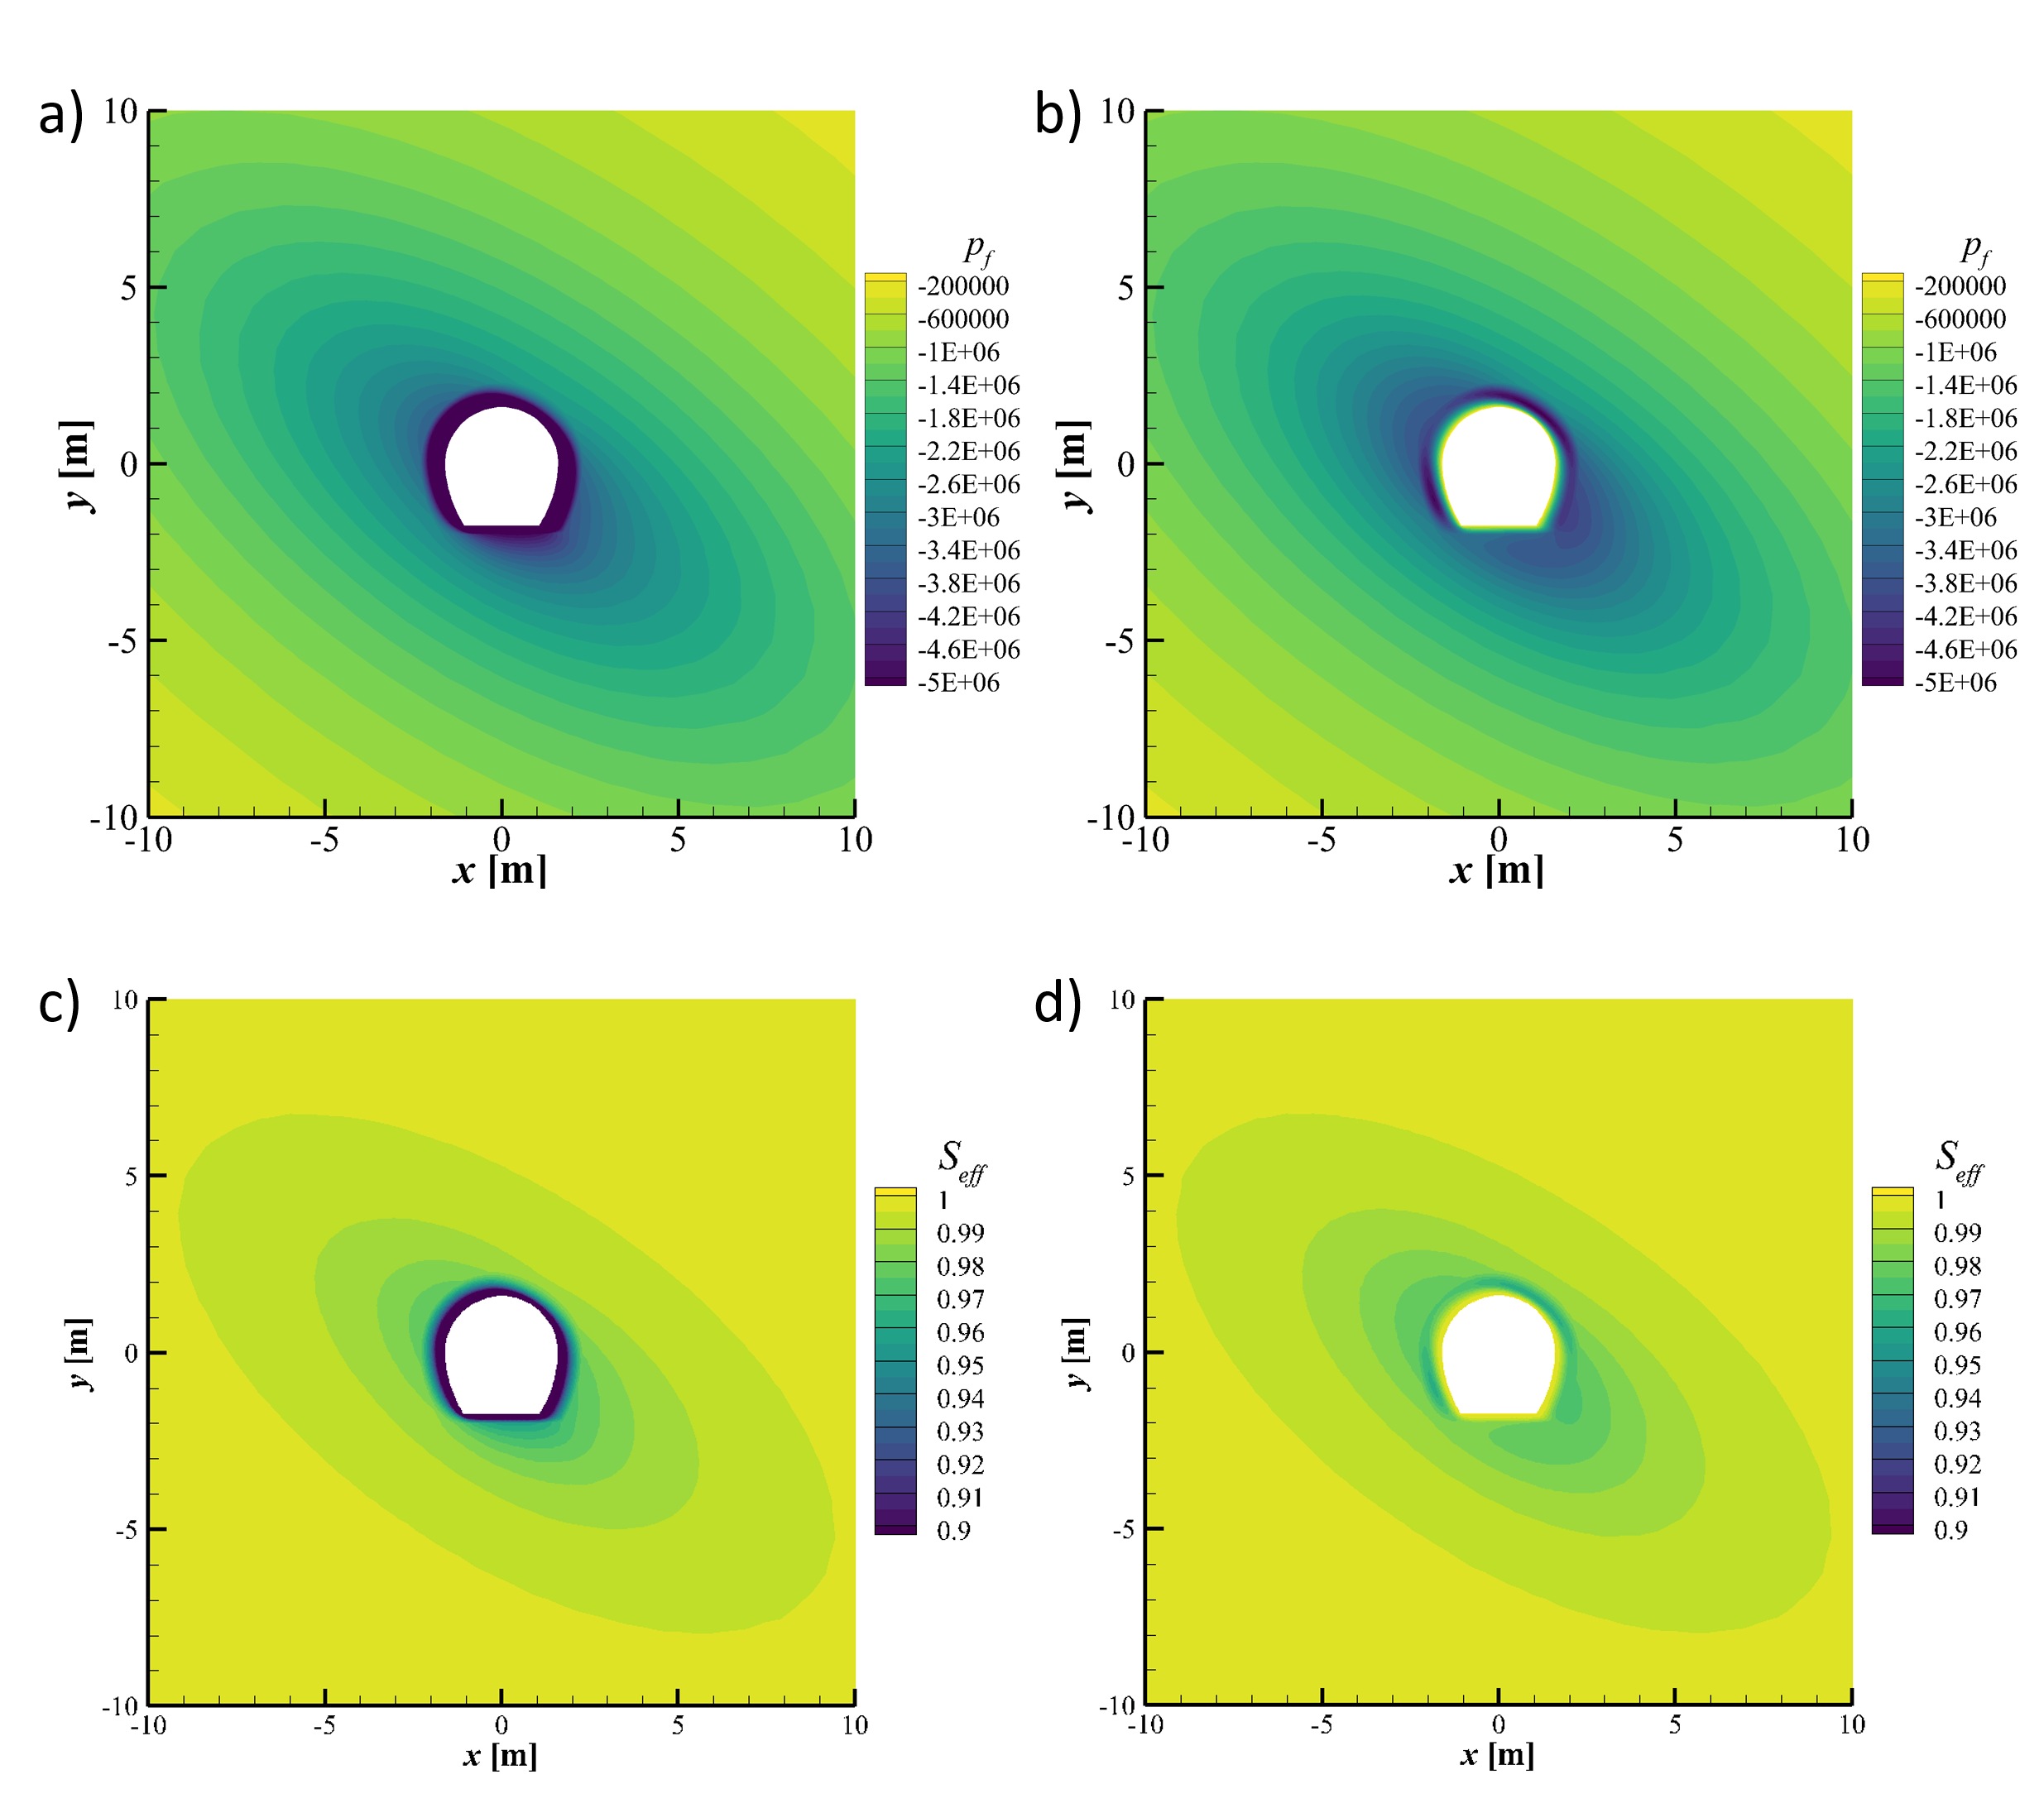
\includegraphics[width=\textwidth, trim=0.4cm 0.2cm 0.2cm 0, clip]{./figures/MEX10_results_pf_S.png}
\caption{Well-developed pattern of seasonally varying quantities fluid pressure (in Pa) and effective saturation. a) fluid pressure at $t=19.5\text{a}$, and b) fluid pressure at $t=20\text{a}$, c) effective saturation at $t = 19.5\text{a}$ and d) effective saturation at $t=20\text{a}$. The figures show a zoom into figure \ref{fig:bc}.}
\label{fig:results}
\end{figure}
%

%%%%%%%%%%%%%%%%%%%%%%%%%%%%%%%%%%%%%%%%%%%%%%%%%%%%%%%%%%%%%%%%%%%%%%%%%%%%%%%%%%%%%%%%%
\subsubsection{Comparison of OGS-5 and OGS-6}\label{sec:mex10_ogs5_vs_ogs6}
%%%%%%%%%%%%%%%%%%%%%%%%%%%%%%%%%%%%%%%%%%%%%%%%%%%%%%%%%%%%%%%%%%%%%%%%%%%%%%%%%%%%%%%%%

A more detailed insight into the evolution of the the desaturated rock surrounding the niche is revealed by plotting $p_f$ and $S_\text{eff}$ probed over time at four different points around the niche. This analysis is shown in Figure \ref{fig:cf_P_S} together with the locations of the sampling points as an inset. The seasonal variations are clearly visible, and the plot reaches a quasi-steady state after 15 years of simulation time. Hence, we conclude that the simulation ran long enough to reach a quasi-steady state for the zone surrounding the niche. Note, however, that these data were collected at locations 3 m away from the niche center in both, horizontal and vertical direction. For probing locations farther away from the niche, it takes longer  to reach a steady state. This state, however, will be closer to fully saturated conditions the farther one moves away from the niche into the undisturbed rock. 

It is now interesting to compare the results from both simulation codes, OGS-5 and OGS-6, to verify whether or not the results have changed after the new implementation of \eqref{eq:richards} in OGS-6. Hence, we show a direct comparison of the simulation results generated by OGS-5 and OGS-6 in the same figure (Figure \ref{fig:cf_P_S}). As desired, all data curves collapse for OGS-5 and OGS-6 at the four different locations for the time simulated. 

%
\begin{figure}[t]
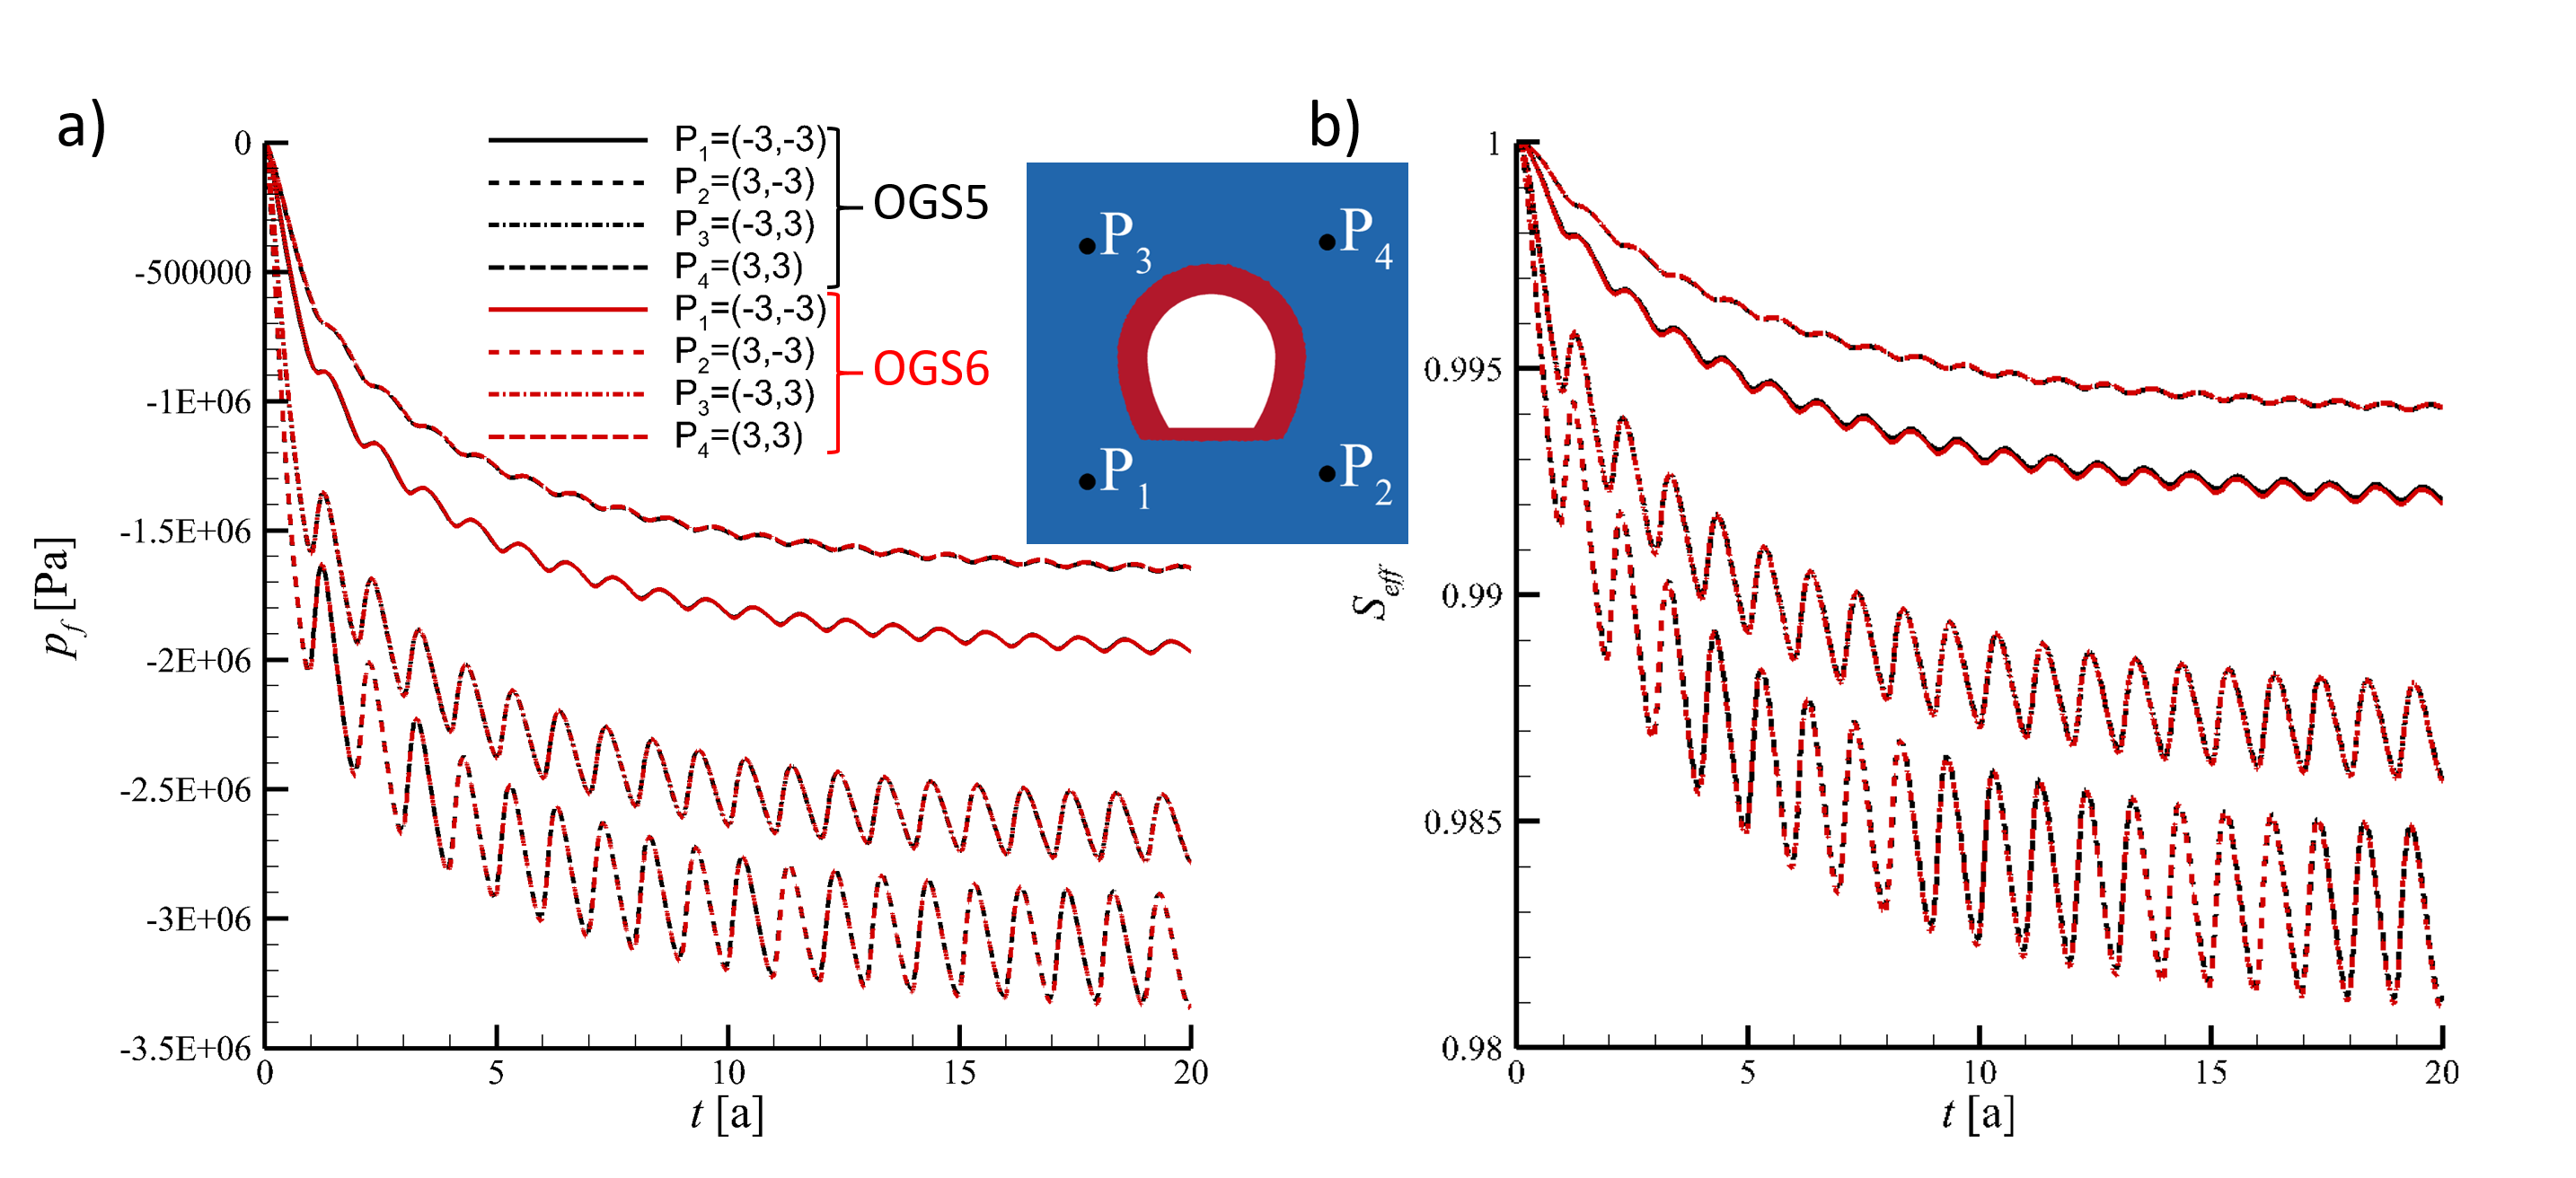
\includegraphics[width=\textwidth, trim=0.4cm 0.2cm 0.2cm 0, clip]{./figures/MEX10_cf_P_S.png}
\caption{Physical quantities probed over time at four different locations surrounding the niche for OGS-5 (black) and OGS-6 (red): a) Fluid pressure and b) effective saturation.  The inset shows the location of the sampling points relative to the niche. The results collapse for OGS-5 and OGS-6.}
\label{fig:cf_P_S}
\end{figure}
%

For a more quantitative comparison, we compute the relative deviation
%
\begin{equation}\label{eq:error}
\epsilon_\theta = \frac{\theta^{OGS5}-\theta^{OGS6}}{\theta^{OGS5}}
\end{equation}
%
where $\theta$ is a quantity of interest, e.g. $p_f$ or $S_\text{eff}$. The two-dimensional plot of the error is shown in Figure \ref{fig:error} for both of these quantities at time $t=20\text{a}$. Far away from the wall of the niche, the error remains small (below $0.1\%$). However, we obtain that OGS-6 slightly underestimates the pressure in the EDZ compared to OGS-5 (Figure \ref{fig:error}a). This is most pronounced at the edges that are not pointing in the main direction of the anisotropy, i.e. at the top right and bottom left edges of the wall. Similarly, we see deviations for the saturation, but here, $S_\text{eff}$ is underestimated at the wall and at the transition from the EDZ to the undisturbed rock, whereas it is overestimated in OGS-6 compared to OGS-5 within the rest of the EDZ (Figure \ref{fig:error}b).

\begin{figure}[t]
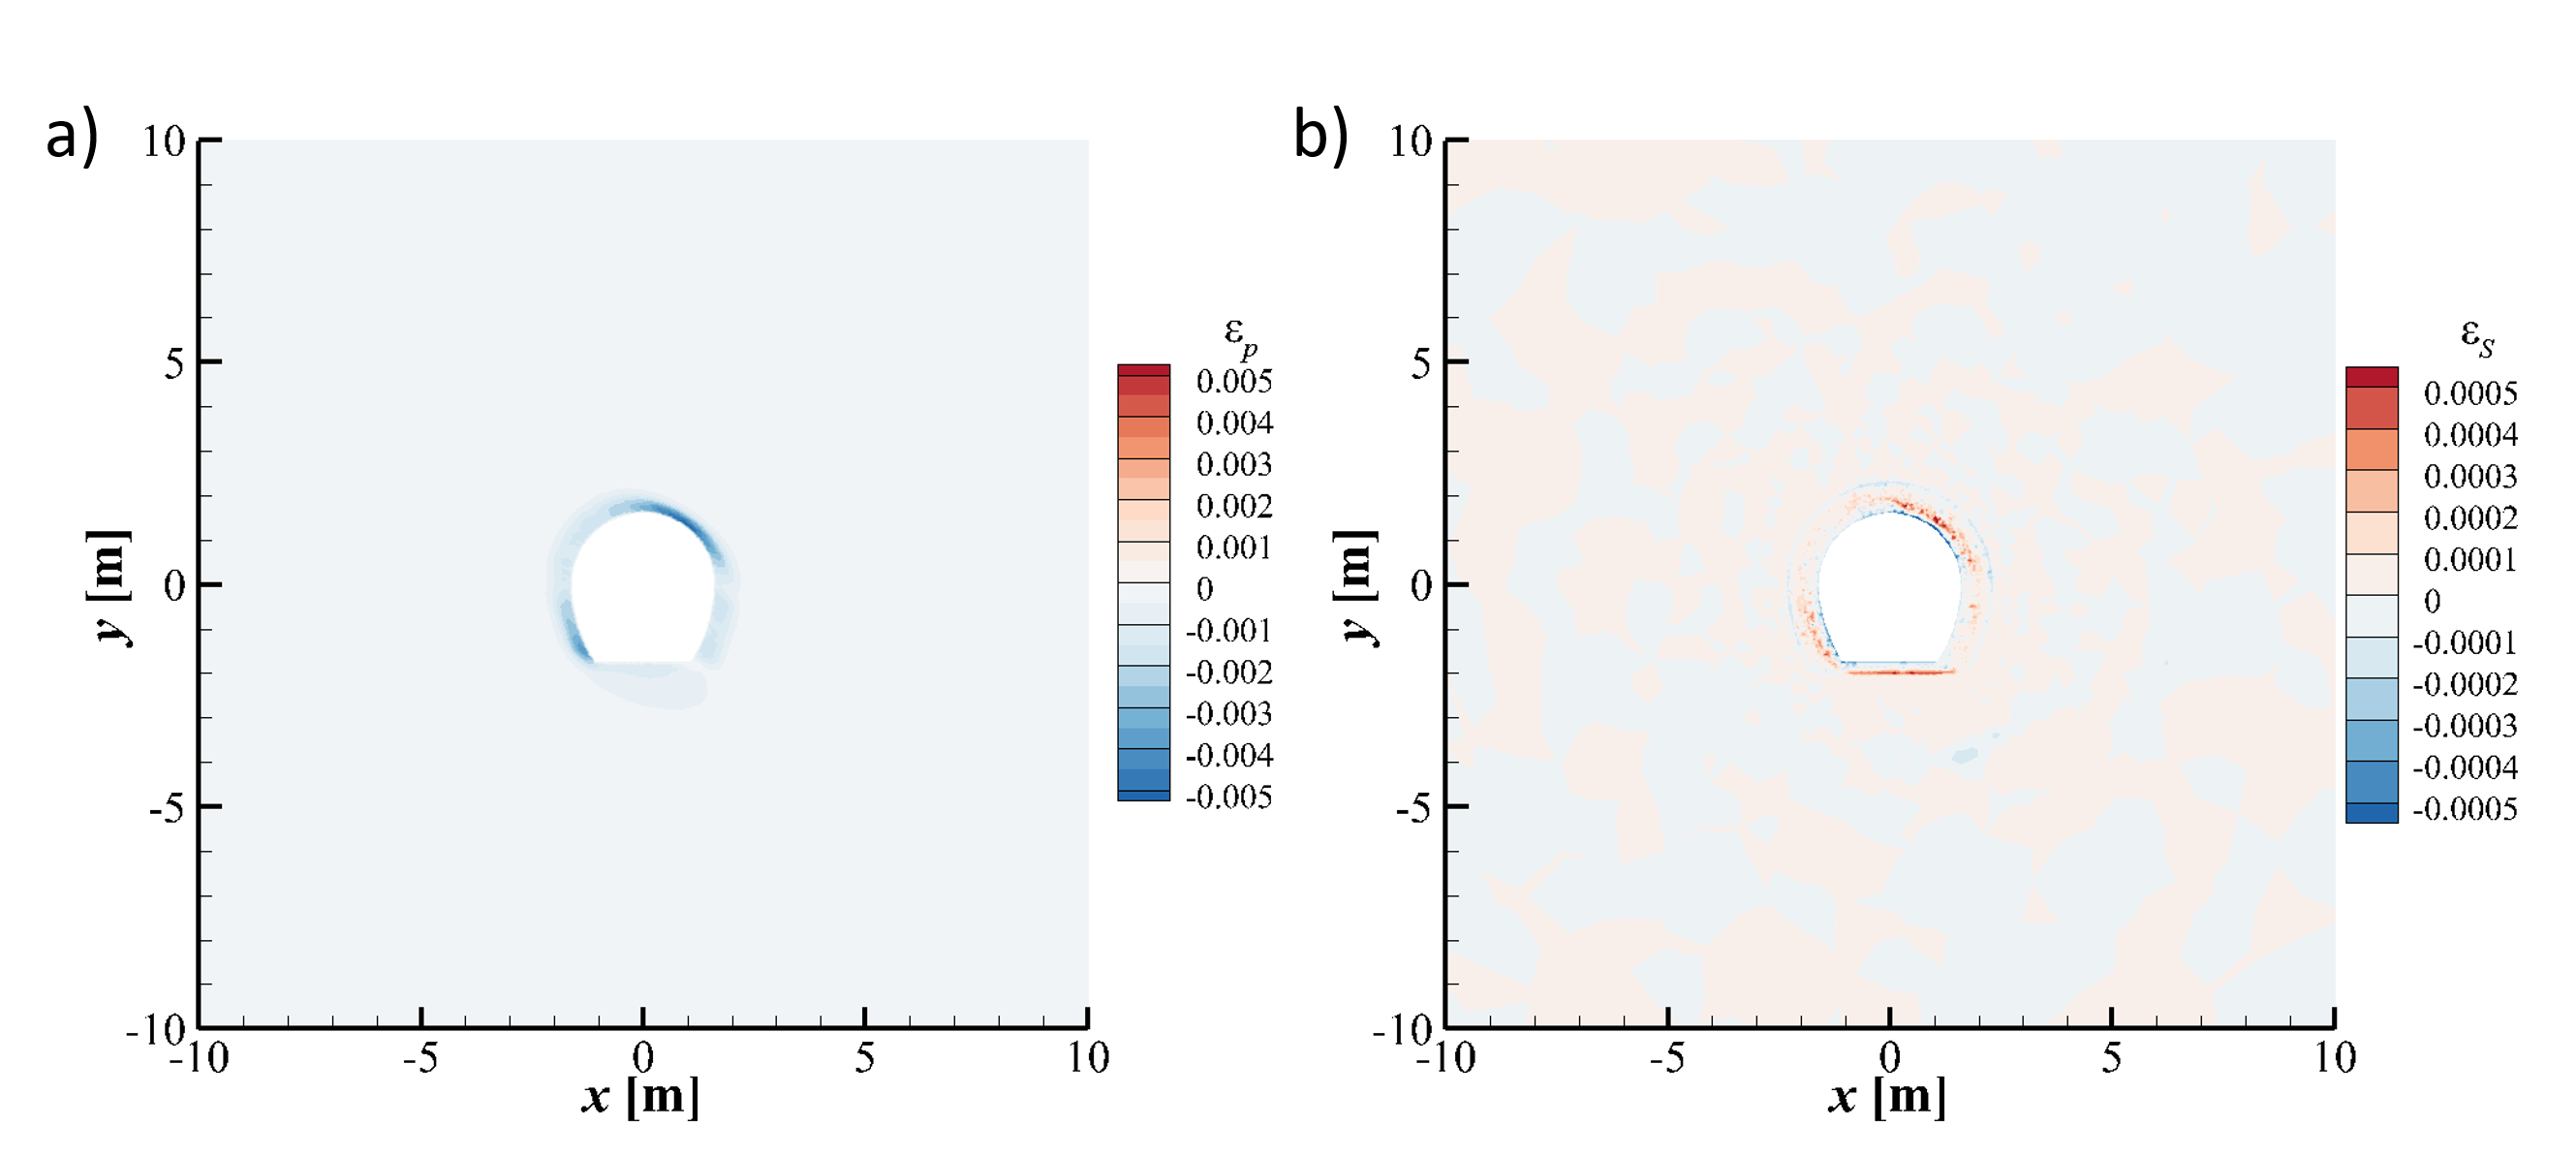
\includegraphics[width=\textwidth, trim=0.6cm 0.0cm 0.0cm 0.2cm, clip]{./figures/MEX10_cf_P_S_2D.png}
\caption{Deviation between OGS-5 and OGS-6 after 20 years of simulation time. a) Fluid pressure and b) effective saturation.}
\label{fig:error}
\end{figure}

Nevertheless, the maximum and minimum deviations as well as the RMSE
\begin{equation}\label{eq:RMSE}
\left \langle \left \lvert \overline{\epsilon}_\theta \right \rvert \right \rangle = \text{RMSE}=\frac{1}{N_\text{nodes}}\sum_{i=1}^{N_\text{nodes}} \sqrt{\epsilon_\theta^2}
\end{equation}
remain below $0.1\%$  (Table \ref{tab:error}). Here, RMSE is the Root Mean Square Error, $i$ is the index of the nodes, and $N_\text{nodes}$ is the total number of nodes of the computational mesh. These small deviations were deemed to be acceptable for the present scenario given that the simulation had run more than twenty cycles of desiccation/saturation.  This is especially true considering the different convergence criteria used for the two different codes (Table \ref{tab:solver}). 

\begin{table}
 \caption{Deviations observed when comparing OGS-5 with OGS-6 for the RF model.\label{tab:error}}
\begin{center}
\begin{tabular}{ l | c | c | c }
 Quantity			& $\min{(\epsilon)}$ 	& $\max{(\epsilon)}$	 & RMSE  \\
 \hline
 $p_f$ & -0.0054 	& 0.0 		& $5.52\cdot 10^{-5}$\\ 
 $S_\text{eff}$ & -0.0012 & 0.0078	& $6.77\cdot 10^{-4}$\\		
\end{tabular}
\end{center}
\end{table}

%%%%%%%%%%%%%%%%%%%%%%%%%%%%%%%%%%%%%%%%%%%%%%%%%%%%%%%%%%%%%%%%%%%%%%%%%%%%%%%%%%%%%%%%%
\subsubsection{Convergence study in space and time in OGS-6}
%%%%%%%%%%%%%%%%%%%%%%%%%%%%%%%%%%%%%%%%%%%%%%%%%%%%%%%%%%%%%%%%%%%%%%%%%%%%%%%%%%%%%%%%%
The rate of convergence is a very important property to judge the consistency of a numerical procedure. A consistent procedure approaches the analytical solution of the problem with increasing resolution in space and time \cite{ferziger2012}.  For an efficient numerical scheme, the rate of convergence should be equal to or greater than unity, i.e. dividing the resolution by a factor of two should also decrease the error by at least a factor of two with respect to the reference solution. By comparing the numerical solution to some reference solution, one can also infer information about the minimum resolution required to obtain acceptable results. While the rate of convergence is often times determined under ideal conditions, i.e. on a regular Cartesian grid for an idealized problem, we apply the procedure to the present case of a niche surrounded by rock of two material groups, anisotropic permeability and cyclic boundary conditions for the fluid pressure at the walls of the niche to analyze a more realistic scenario. This is done in two consecutive steps: first we present order of convergence in time and then in space. 

\subsubsection*{Convergence study time}
To analyze the consistency in time, we use the exact same computational setup described in Section \ref{sec:model_RF} above. While the results generated with this setup and presented in Sections \ref{sec:well_developed} and \ref{sec:mex10_ogs5_vs_ogs6} were computed with $\Delta t = 21,400$ s, we now vary the time integration interval within the range $1350 \, \text{s} \leq \Delta t  \leq 345,600$ s. We ran a total of nine simulations doubling $\Delta t$ for each simulation. This yields an integration time interval ranging between 24 minutes and 4 days. The run with the smallest time integration interval, i.e. $\Delta t = 1350$ s, was chosen as a reference solution, since there is no analytical solution available for the current setup.

\begin{figure}[t]
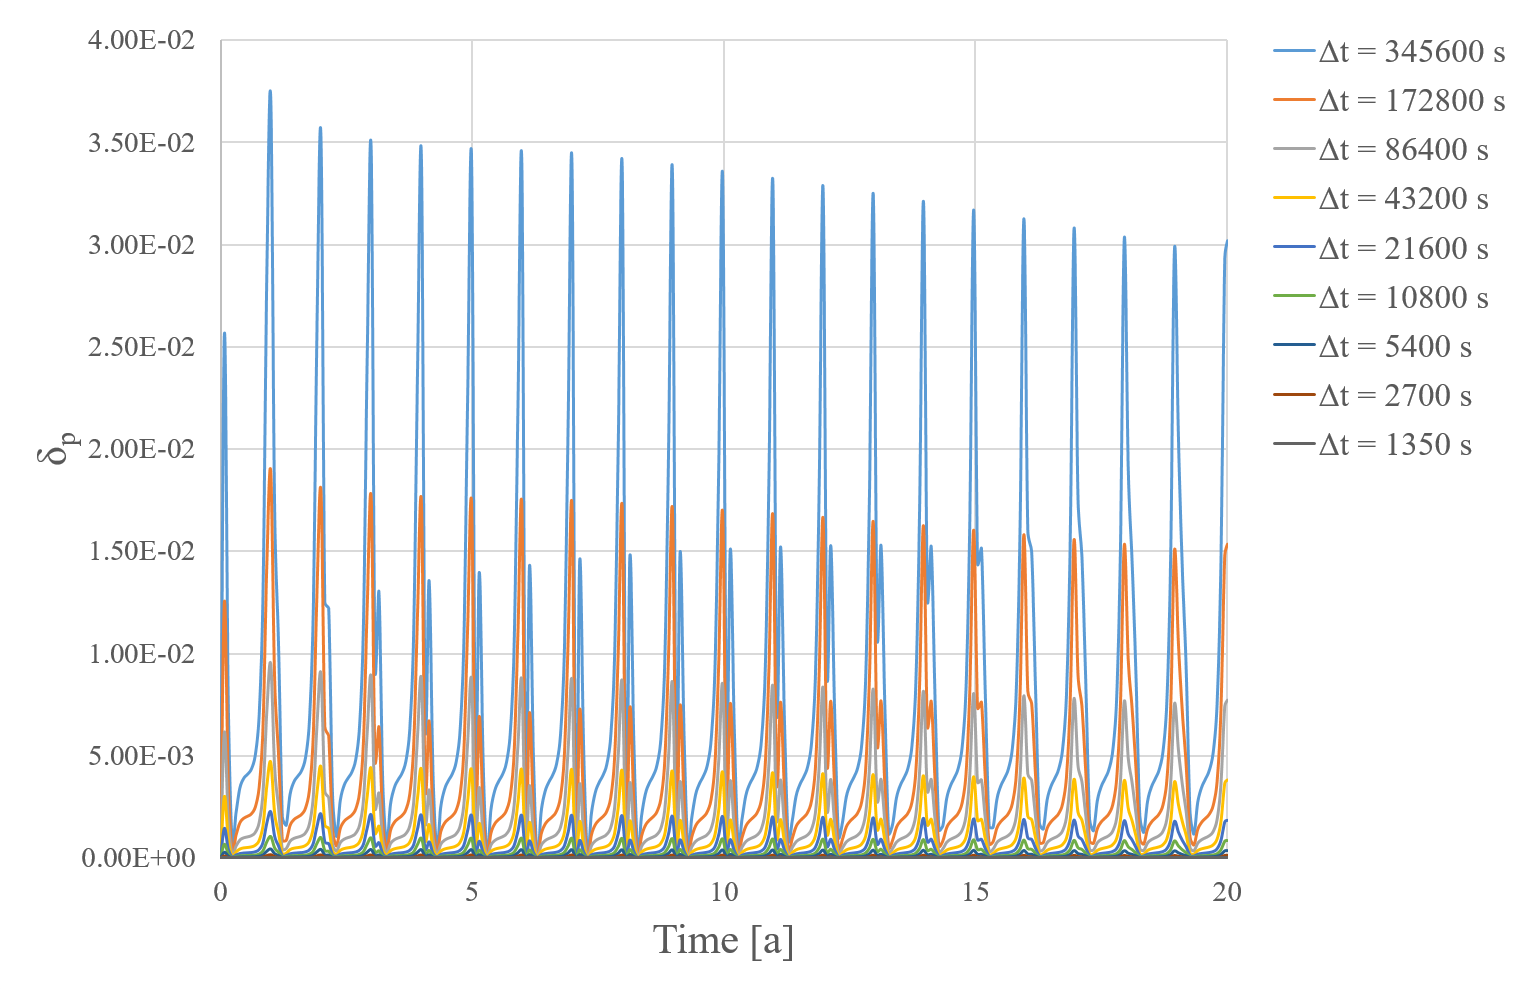
\includegraphics[width=\textwidth]{./figures/MEX10_convergence_error.png}
\caption{Deviation between the simulations using different time discretizations $\Delta t$ at sampling point $P_1 = (2.0,0.0)$ (cf. inset in Figure \ref{fig:convergence_time}). }
\label{fig:convergence_error}
\end{figure}

As a next step, we define sampling points, for which we probe data for fluid pressure and effective saturation over time.  Since Figure \ref{fig:error} suggested that deviations between OGS-5 and OGS-6 were largest at the transition zone from the undisturbed rock (material ID 1) to the EDZ (material ID 2), we chose four different locations inside the EDZ surrounding the niche at this critical distance, which is 2 m away from the domain center for $P_1, P_2$ and $P_3$ and 1.9 m for $P_4$, which is directly located underneath the niche. The  coordinates are sketched in the inset in Figure \ref{fig:convergence_time} and listed in Table \ref{tab:convergence_time}. As a next step, we define the characteristic error
%
\begin{equation}
\delta_\theta(\Delta t) = \left \lvert \frac{\theta(\Delta t) - \theta(\Delta t_\text{ref}) }{\theta(\Delta t_\text{ref})} \right \rvert \qquad ,
\end{equation}
%
where again $\theta$ represents fluid pressure and effective saturation, respectively, and $\Delta t_\text{ref}= 1350$ s is the time integration interval of the reference run. 

An example of the temporal evolution of $\delta_p$ for $P_1 = (2.0,0.0)$ is given in Figure \ref{fig:convergence_error}. Similar to the observations reported for Figure \ref{fig:bc} above, there is a strong cyclic behavior of the error that depends on the evolution of $p_t$. A peak in $p_t$ corresponds with a maximum deviation of the simulation result from the reference solution. This behavior was expected as a coarser discretization tends to smoothen out maximum values of a continuous function.  For a given $\Delta t$, the deviations slightly decrease over time and decreasing $\Delta t$ reduces the deviations from the reference solution substantially for all values of $\Delta t$ investigated. Similar results were obtained for the other three sampling points.

\begin{figure}[t]
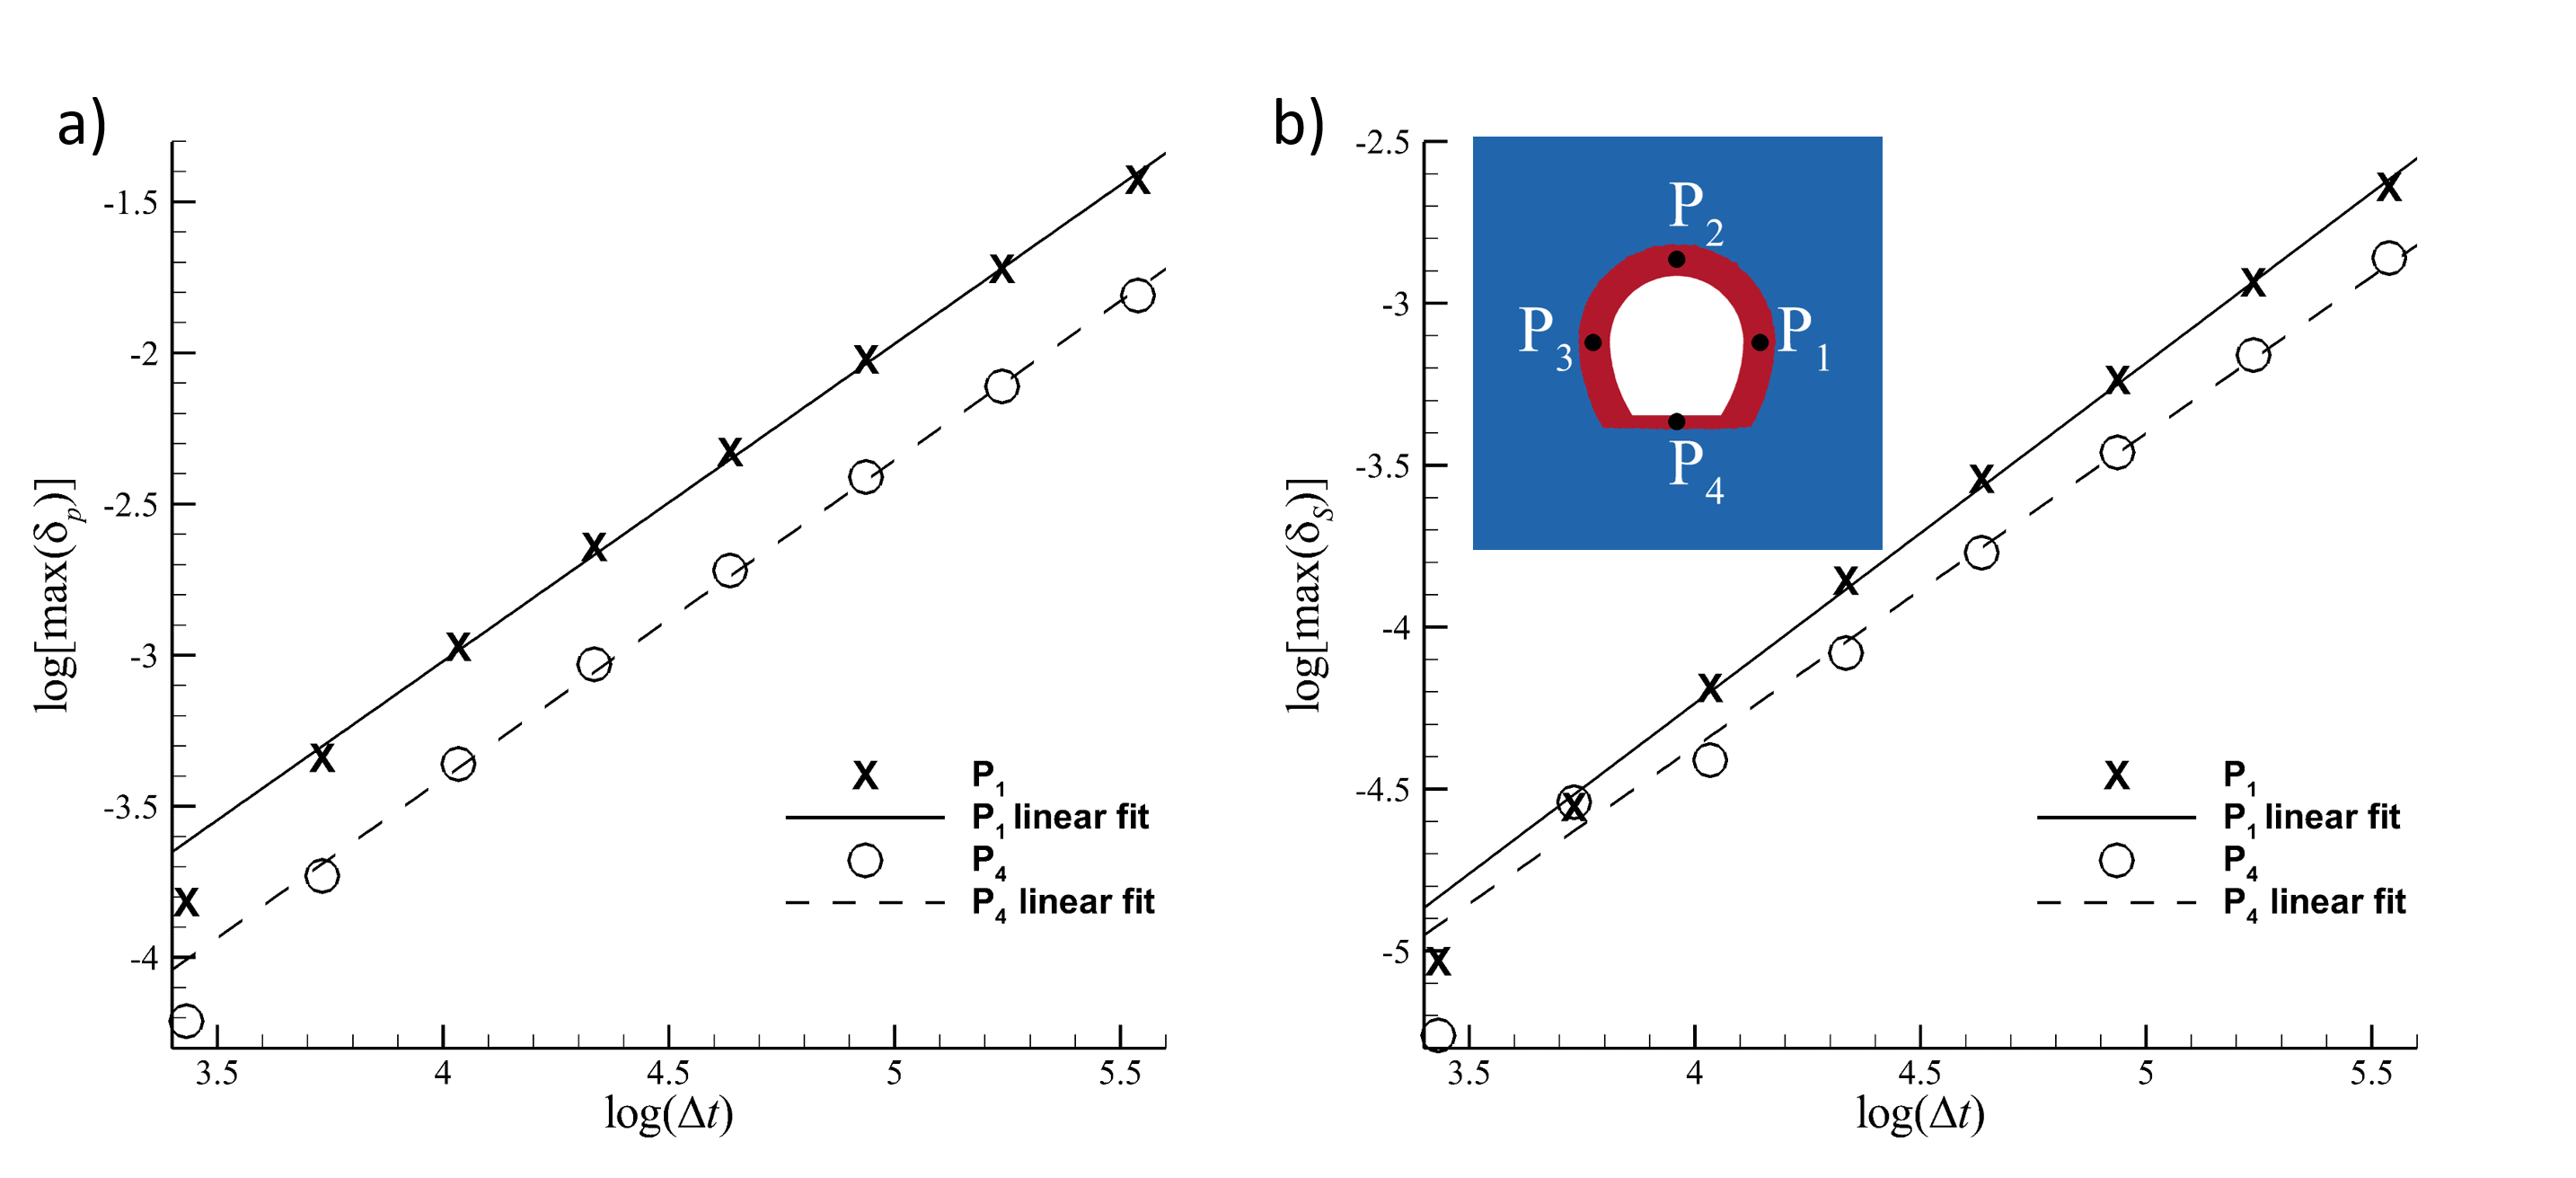
\includegraphics[width=\textwidth]{./figures/MEX10_convergence_time.png}
\caption{Order of convergence in time for two characteristic sampling points on a log-log scale. The error increases with increasing $\Delta t$. a) Fluid pressure and b) effective saturation. The inset shows the locations of the analyzed sampling points. }
\label{fig:convergence_time}
\end{figure}

To quantify the deviations from the reference solution, we plot the maximum deviation $\max{(\delta_\theta)}$ against $\Delta t$ in a log-log plot in Figure \ref{fig:convergence_time}. As already observed in Figure \ref{fig:convergence_error}, all data points follow the same trend of decreasing error with decreasing time step size. Note that we have only plotted results for $P_1$ and $P_4$, because the data from $P_2$ and $P_3$ collapsed with the data from $P_1$. The offset of $P_4$ from the rest of the sampling points is probably due to the slight difference in distance from the center of the domain and the flat bottom wall of the niche.


Finally, we determine the order of convergence by computing the linear fit of $y=ax + b$ for the log-log plot in Figure \ref{fig:convergence_time}. In fact, the linear fit is a very good approximation of the data presented in that figure, so that the fitting parameter $a$, which is the slope of the linear regression, serves very well to determine the order of convergence. Note that we have excluded the first data point (with the lowest value of $\Delta t$) from the fit, because it is slightly offset due to the fact that the reference case using $\Delta t_\text{ref}$ does not represent an analytical solution as would have been desirable for a mathematically rigorous convergence analysis. The values of $a$ and $b$ for the fluid pressure and the effective saturation are summarized in Table \ref{tab:convergence_time} for all four sampling points investigated.  For both physical quantities, the slope turns out to be 1.05 on average, which proves that the current time integration scheme of the "Richards Flow" model in OGS-6 is an efficient implementation of the {\em Backward Euler} scheme; a scheme that is known to be of first order \cite{ferziger2012}. 

\begin{table}
 \caption{Order of convergence in time extracted from the linear fit $y=ax + b$ as given in the log-log plot of Figure \ref{fig:convergence_time} at the different sampling points shown in the same figure.\label{tab:convergence_time}}
 \begin{center}
\begin{tabular}{ l || r | r ||  r | r }
 					& \multicolumn{2}{c ||}{Pressure} & \multicolumn{2}{c}{Saturation} \\
Sampling point		& $a$ 		& $b$ 	    & $a$		& $b$ \\
 \hline
 $P_1=(2.0,0.0)$ 	& 1.051 	& -7.222 	& 1.052 	& -8.441 	\\ 
 $P_2=(0.0,2.0)$ 	& 1.050  	& -7.217	& 1.107 	& -8.715 	\\ 
 $P_3=(-2.0,0.0)$ 	& 1.046 	& -7.192	& 1.054 	& -8.431 	\\ 
 $P_4=(0.0,-1.9)$ 	& 1.054 	& -7.622	& 0.968 	& -8.242 	\\ 
\end{tabular}
\end{center}
\end{table}


\subsubsection*{Convergence study space}
Similar to the convergence study in time described above, we use the computational setup described in Section \ref{sec:model_RF} to repeat the simulations on different grids with different resolution. This time, the time integration interval was kept constant at $\Delta t = 21,400$ s, but the number of grid nodes $N_\text{nodes}$ was varied within the range $3613 \leq N_{nodes} \leq 60,845$. Note that we switched from a triangulated domain to a tetrahedral meshing due to its more regular behavior for grid refinements at the walls of the niche. We conducted a total of five simulations, where the simulation with $N_\text{nodes}=3614$ used the coarsest grid (Figure \ref{fig:meshes}a), $N_\text{nodes}= 6500$ is comparable to the triangulated grid with 5463 nodes as shown in Figure \ref{fig:setup}b, while we refined the grid to $N_\text{nodes}=11,045$ (Figure \ref{fig:meshes}b) and $N_\text{nodes}=31,582$, respectively. Again, the finest resolution with $N_\text{nodes}=N_\text{ref}=60,845$ (Figure \ref{fig:meshes}c) serves as the reference run, since there is no analytical solution available. 

It is important to note that the the mesh generator Gmsh \cite{geuzaine2009} does not allow for the exact control over the number of nodes generated for the complex geometry in the present analysis. Hence, we adapt the number of grid cells by refining the spatial discretization at the outer boundary of the domain from 5 m ($N_\text{nodes} = 3613$) to 0.7 m ($N_\text{nodes} = 60,845$). This measure did not refine the grid at the walls of the niche in the same systematic manner, because the nodes have to coincide with the points defining the polygon course of the complex niche shape. In fact, we obtained the same spatial resolution $\Delta x = 0.0375$ m for the arch of the niche for all simulations, whereas the resolution at the more regular bottom was refined from 0.177 m to 0.034 m. 

\begin{figure}[t]
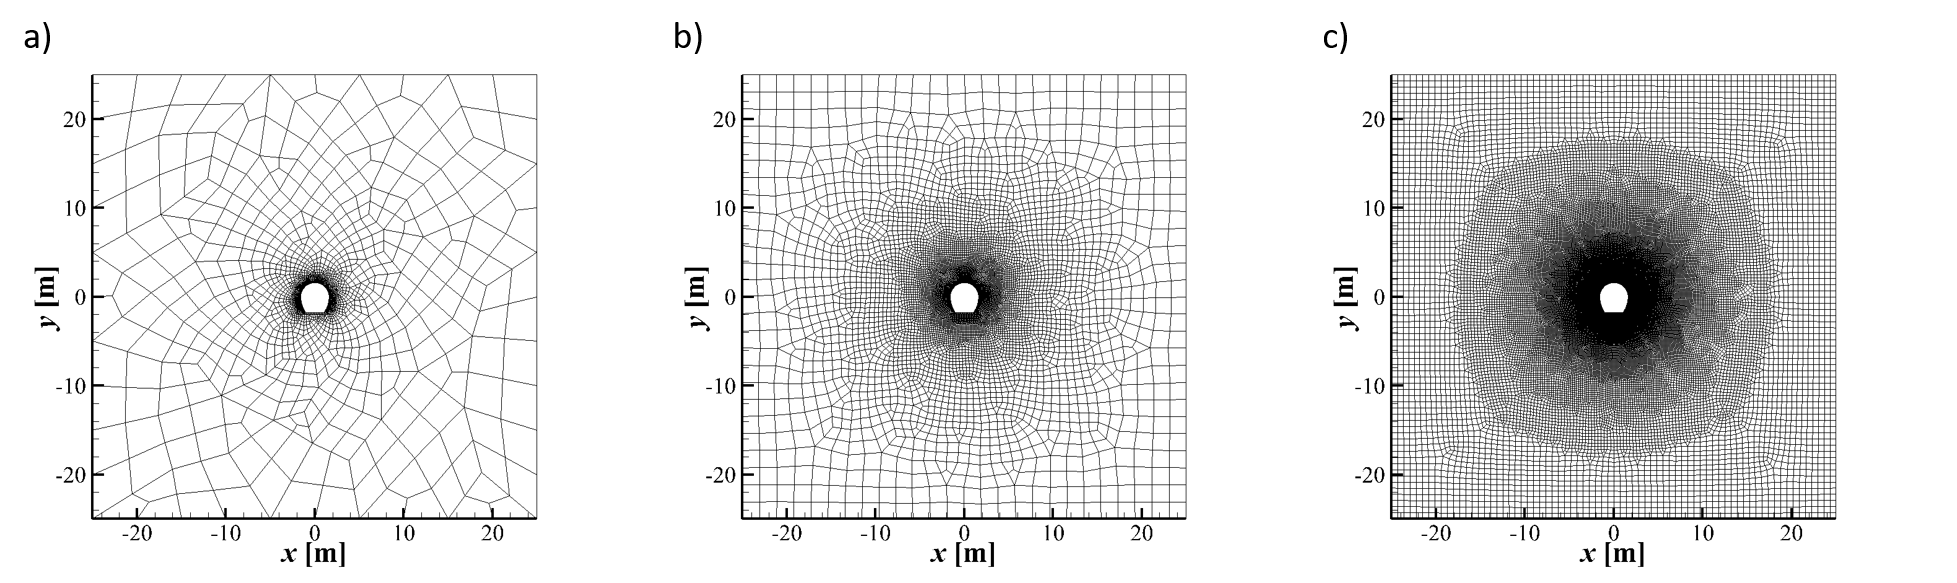
\includegraphics[width=\textwidth, trim=0.4cm  0.0cm 0 0.3cm, clip]{./figures/MEX10_meshes.png}
\caption{Examples of the meshes used to conduct the grid convergence. a) $N_\text{nodes}=3613$, which was the coarsest grid employed, b) $N_\text{nodes}=11,047$, c) $N_\text{nodes}=60,845$, which was the finest grid employed.}
\label{fig:meshes}
\end{figure}

We compute the error as 
%
\begin{equation}
\delta_\theta(N_\text{nodes}) = \left \lvert \frac{\theta(N_\text{nodes}) - \theta(N_\text{ref}) }{\theta(N_\text{ref})} \right \rvert \qquad ,
\end{equation}
%
to quantify the deviation of the results with respect to a given reference mesh, here the finest spatial resolution with $N_\text{ref}=60,845$ nodes. We defined four sampling points that were moved farther into the undisturbed rock to a distance of 4 m away from the center of the niche (Figure \ref{fig:convergence_space}). This became necessary as the polyline defining the boundary between the two material IDs, which is about 2 m away from the center of the niche, predefines specific nodes. Sampling in this area would influence the convergence behavior of the simulations. Subsequently, we used a interpolation routine provided by the software TecPlot \cite{tecplot2019} to obtain data over time at these sampling points for all the simulations with different grid resolution. Due to the remeshing, however, the sampling points' location no longer coincide with the node locations. Hence, if the grid is too coarse, those sampling points can be closer or farther away from the next node location depending on the mesh. For these cases, the interpolation routine offered by the postprocessing software TecPlot will heavily influence the results and conclusions about the order of convergence will no longer be possible.


\begin{figure}[t]
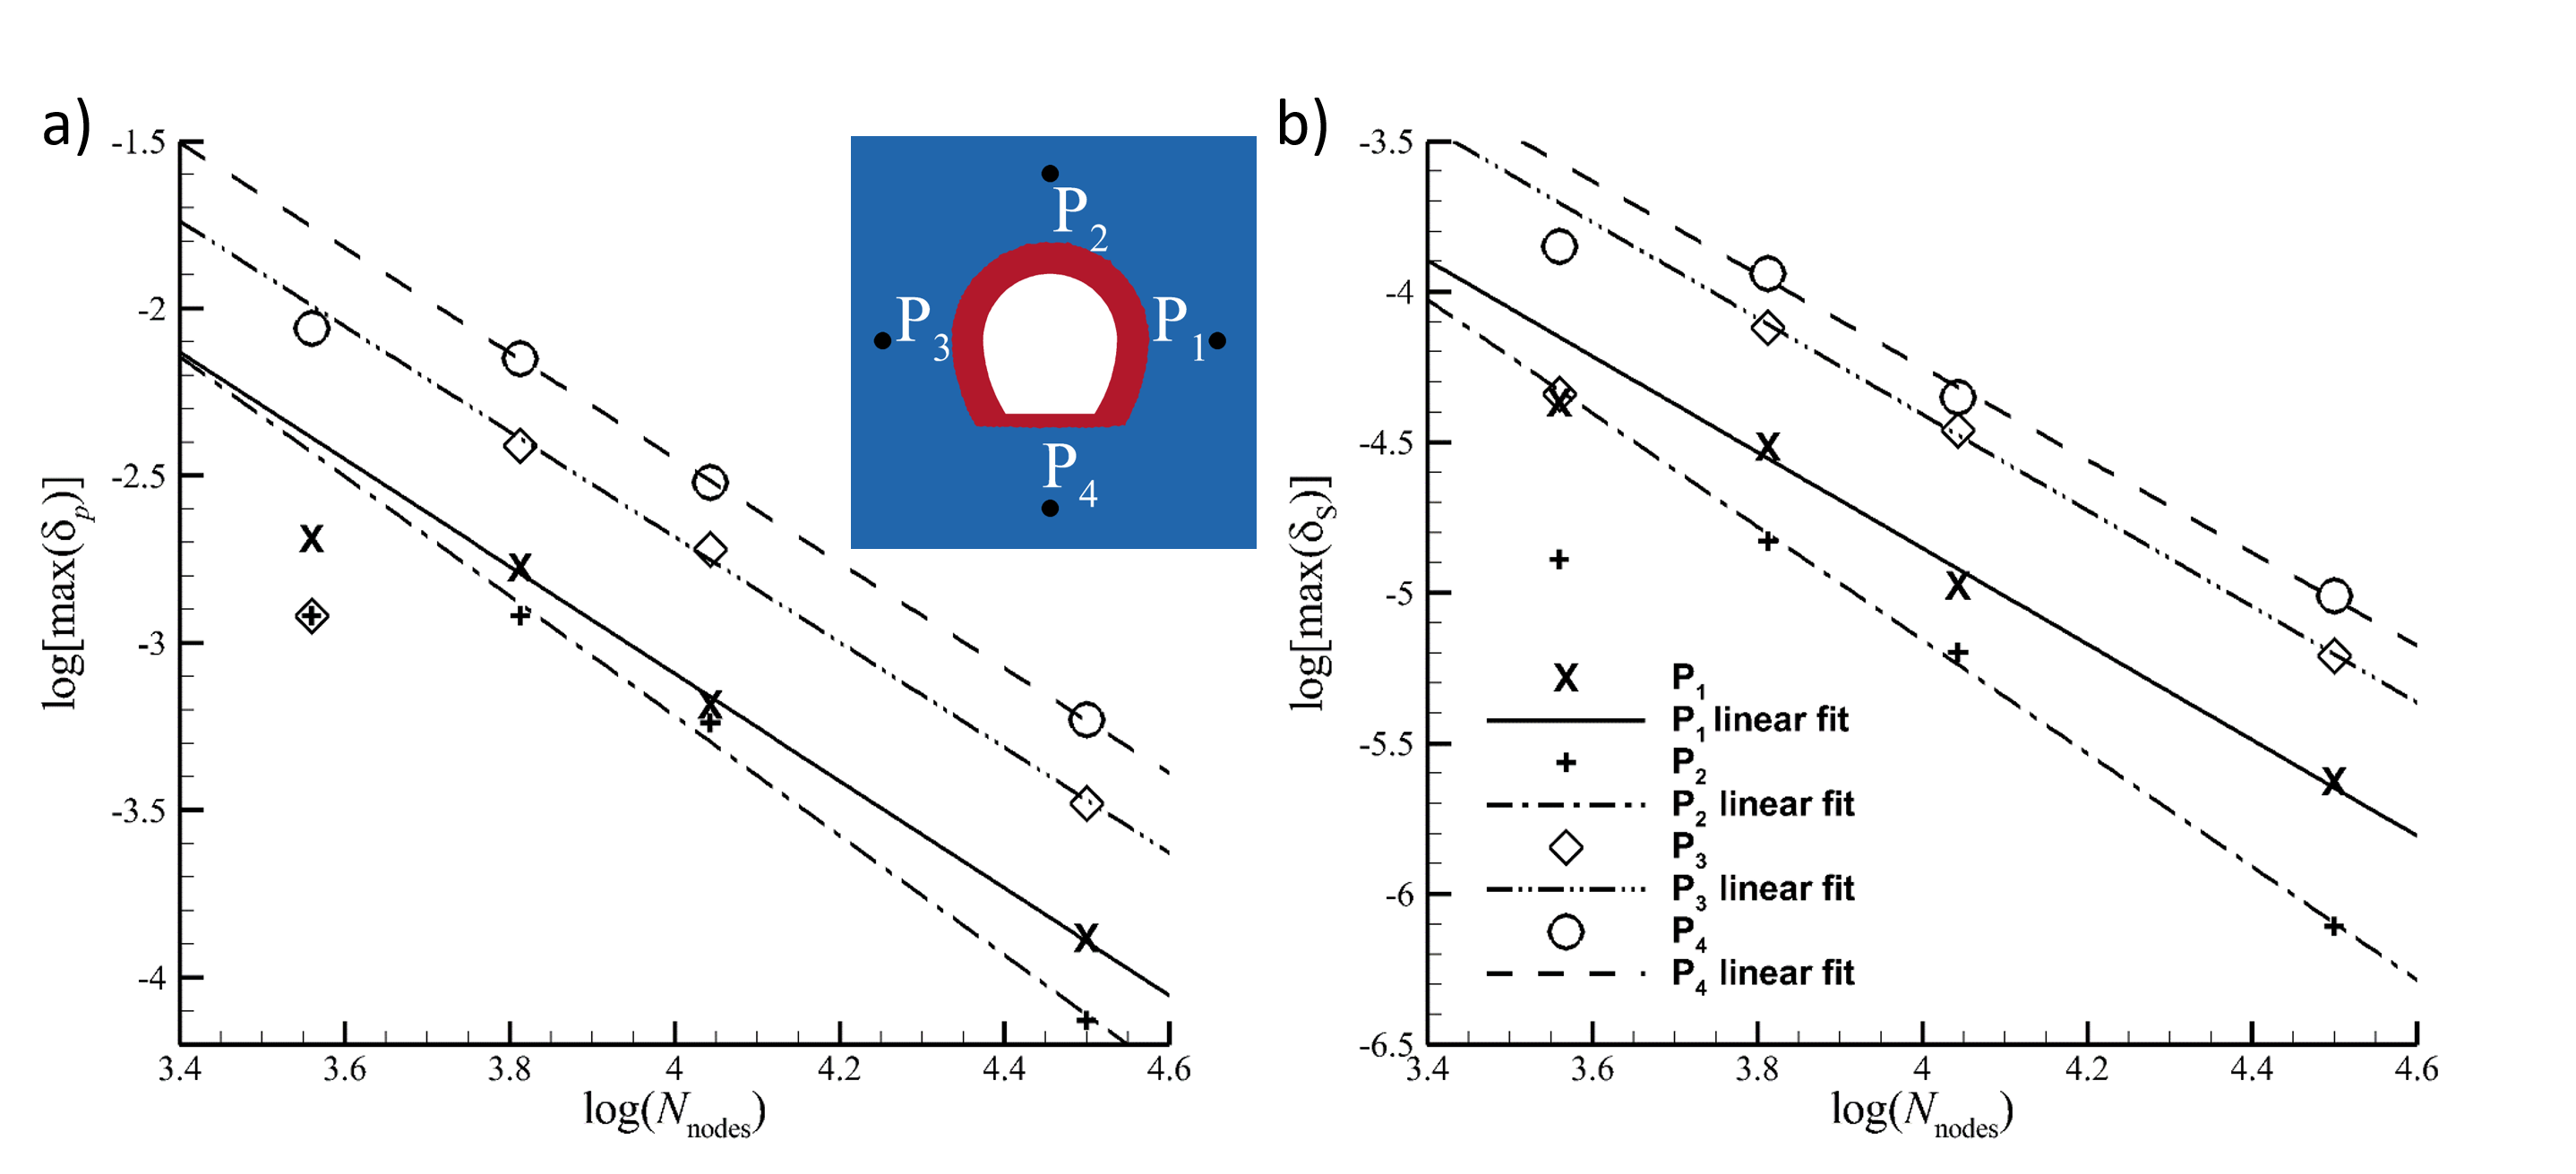
\includegraphics[width=\textwidth, trim=0.3cm  0.0cm 0 0.0cm, clip]{./figures/MEX10_convergence_space.png}
\caption{Order of convergence in space for four characteristic sampling points on a log-log scale. The error decreases with increasing number of grid cells $N_\text{nodes}$. a) Fluid pressure and b) effective saturation. The inset shows the locations of the analyzed sampling points. }
\label{fig:convergence_space}
\end{figure}

After probing the data at the different sampling points, we obtain results very similar to Figure \ref{fig:convergence_error}. The resulting convergence behavior with increasing grid resolution is shown in Figure \ref{fig:convergence_space} for both fluid pressure and effective saturation. Overall, the error decreases with increasing grid resolution. This is true for both quantities recorded at all four sampling points, except for the values recorded for the coarsest mesh with $N_\text{nodes}=3614$. Apparently, the interpolation routine of the postprocessing software has a big impact on the quality of the results of this run. It was therefore decided to exclude these data from the linear regression analysis and the grid with $N_\text{nodes} = 3613$ nodes was deemed to be too coarse to obtain meaningful results.

\begin{table}
 \caption{Order of convergence in space extracted from the linear fit $y=ax + b$ as given in the log-log plot of Figure \ref{fig:convergence_time} at the different sampling points shown in the same figure.\label{tab:convergence_space}}
 \begin{center}
\begin{tabular}{ l || r | r ||  r | r }
 					& \multicolumn{2}{c ||}{Pressure} & \multicolumn{2}{c}{Saturation} \\
Sampling point		& $a$		&$b$		& $a$		& $b$ \\
 \hline
 $P_1=(4.0,0.0)$ 	& -1.603 	& 3.321 	& -1.593  	& 1.521 	\\ 
 $P_2=(0.0,4.0)$ 	& -1.789 	& 3.938		& -1.883	& 2.374 	\\ 
 $P_3=(-4.0,0.0)$ 	& -1.574	& 3.611		& -1.596 	& 1.975 	\\ 
 $P_4=(0.0,-4.0)$ 	& -1.571 	& 3.836		& -1.543 	& 1.921 	\\ 
 
\end{tabular}
\end{center}
\end{table}

Nevertheless, after excluding two out of five simulations (with the coarsest being too coarse and the finest being the reference case), we are able to perform a linear regression analysis $y = ax + b$ with a very high correlation on the remaining three data points for the four different sampling locations. The slope of this linear regression, which is the fitting parameter $a$, then yields the order of convergence. The results of this analysis is summarized in Table \ref{tab:convergence_time}. Note the change of sign in $a$ as we obtain a decreasing error with an increase in the number of nodes. For both quantities recorded at all four points, the order of convergence in space averages out to be 1.64, which is well above 1. Hence, we conclude that improving the grid resolution can improve the simulation results drastically.

%%%%%%%%%%%%%%%%%%%%%%%%%%%%%%%%%%%%%%%%%%%%%%%%%%%%%%%%%%%%%%%%%%%%%%%%%%%%%%%%%%%%%%%%%%%%
\subsection{Unsaturated single-phase coupled with linear elasticity ("Richards Mechanics", RM)}\label{sec:RM}
\subsubsection{Model description}\label{sec:model_RM}
%%%%%%%%%%%%%%%%%%%%%%%%%%%%%%%%%%%%%%%%%%%%%%%%%%%%%%%%%%%%%%%%%%%%%%%%%%%%%%%%%%%%%%%%%%%%
The dynamic boundary conditions of $p_t$ described for the simulations using the RF-model yields changes in local saturation. It is well known, however, that changes in fluid pressure will also have effects on the rock matrix of the Opalinus clay \cite{wild2017}. To account for these processes, the hydraulic model described in Section \ref{sec:model_RF} is extended to a coupled hydraulic-mechanical model \cite{lewis1998}. In what follows, this model will be called "Richards Mechanics" (RM). The coupling between the fluid pressure and the local stress is based on the effective stress concept, which states that the total stress is equal to the sum of the pore pressure and the effective stress acting on the solid. This concept was initially developed for saturated porous soils\cite{biot1941,terzaghi1943} and was later extended for unsaturated porous media flows \cite{bishop1963}. 

The coupling of the fluid and the solid phase via the effective stress concept yields the balance of linear momentum:
\begin{equation}\label{eq:linear_momentum}
\boldsymbol{\nabla} \cdot \left( \boldsymbol{\sigma} - \alpha \chi(S) p_f \textbf{I} \right) = 0 \qquad,
\end{equation}
where $\boldsymbol{\sigma}$ is the effective stress tensor, $\alpha$ is the Biot coefficient, $\chi(S)=S$ is a simple model for the Bishop's coefficient and $\textbf{I}$ is the identity matrix. The mass balance for the fluid in a deformable porous medium, hence, becomes:
\begin{equation}\label{eq:mass_balance}
 \phi \frac{\partial S}{\partial t} + S\left(\frac{\phi}{K_f}+\frac{\alpha -\phi}{K_s}\right) \frac{\partial p_f}{\partial t}+ \boldsymbol{\nabla} \cdot \textbf{J}_f + S \alpha \boldsymbol{\nabla} \cdot \frac{\partial \textbf{u}}{\partial t} = 0
\end{equation}
where $K_f$ and $K_s$ are the bulk moduli for the fluid and the solid phase, respectively, and $\textbf{u}$ is the displacement vector of the solid matrix. Furthermore
\begin{equation}
\textbf{J}_f=\frac{k_\text{rel}\textbf{k}}{\mu_f}(\nabla p_f-\rho_f \textbf{g})
\end{equation}
is the fluid mass flux that already appeared in the RF-model \eqref{eq:richards}.
The constitutive relation for the effective stress tensor is the generalized Hooke's law
\begin{equation}\label{eq:hookes_law}
\boldsymbol{\sigma} = \mathds{C} \colon \boldsymbol{\epsilon} \qquad ,
\end{equation}
where we use the Voigt notation to write $\mathds{C}$ the elasticity tensor, and $\boldsymbol{\epsilon}=\frac{1}{2}\left(\nabla \textbf{u} + (\nabla \textbf{u})^T\right)$ is the strain tensor. 

%%%%%%%%%%%%%%%%%%%%%%%%%%%%%%%%%%%%%%%%%%%%%%%%%%%%%%%%%%%%%%%%%%%%%%%%%%%%%%%%%%%%%%%%%
\subsubsection{Comparison of the Richards equation implementation for the two model approaches "Richards Flow" and "Richards Mechanics" in OGS-6}\label{sec:RM_no_M}
%%%%%%%%%%%%%%%%%%%%%%%%%%%%%%%%%%%%%%%%%%%%%%%%%%%%%%%%%%%%%%%%%%%%%%%%%%%%%%%%%%%%%%%%%
The comparison made in Section \ref{sec:mex10_ogs5_vs_ogs6} above is based on the process "Richards Flow" (RF). Since OGS-6 employs a monolithic scheme to solve coupled systems, this analysis does not allow for the conclusion that implementation of the Richards equation \eqref{eq:richards} is verified for all other coupled models as well. Hence, we ran the same simulation using "Richards Mechanics" (RM) to validate the implementation of the Richards equation in OGS-6 for this model. To focus on the Richards equation only, we turn off the hydraulically induced mechanical deformation by choosing a Biot coefficient of $\alpha = 0.0$ and set deformations at all outer boundaries to zero for all directions. Furthermore, we drive the storage term, which is the second term in \eqref{eq:linear_momentum} to zero by setting the bulk moduli to $K_f=K_s=1\cdot 10^{100}\, Pa$. 

\begin{figure}[t]
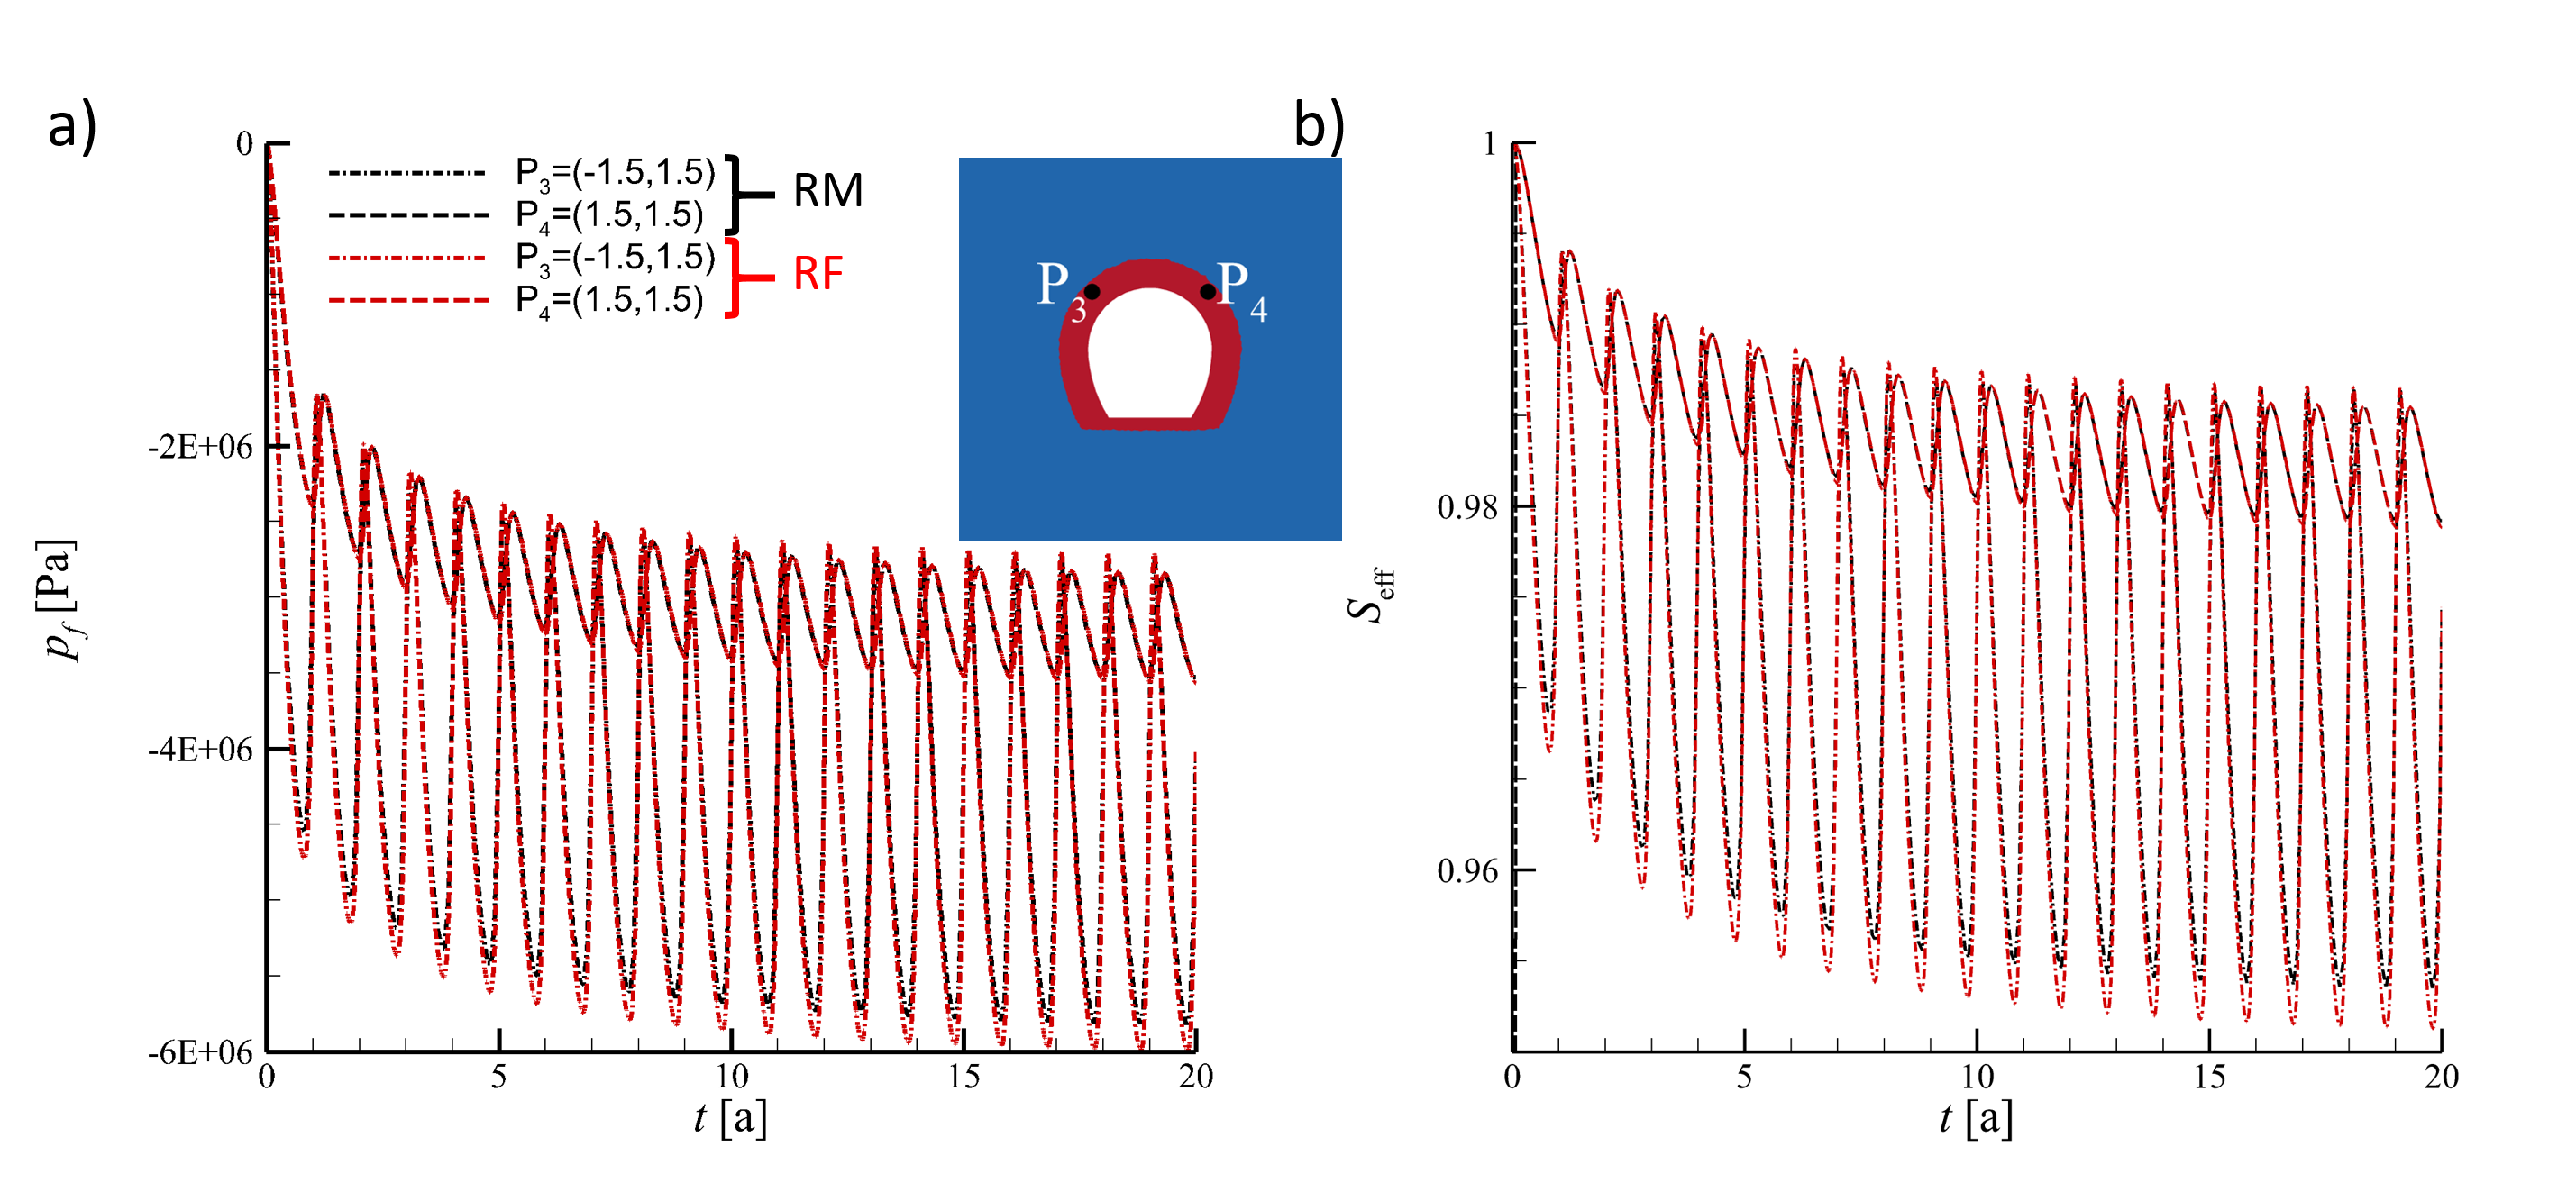
\includegraphics[width=\textwidth]{./figures/MEX10_cf_RF_RM.png}
\caption{Physical quantities probed over time at two characteristic locations for the model approaches 'Richards Flow' (RF, black) and 'Richards Mechanics' (RM, red). a) Fluid pressure and b) effective saturation. The inset shows the location of the sampling points relative to the niche.}
\label{fig:probe_RM_RF}
\end{figure}

\begin{figure}[t]
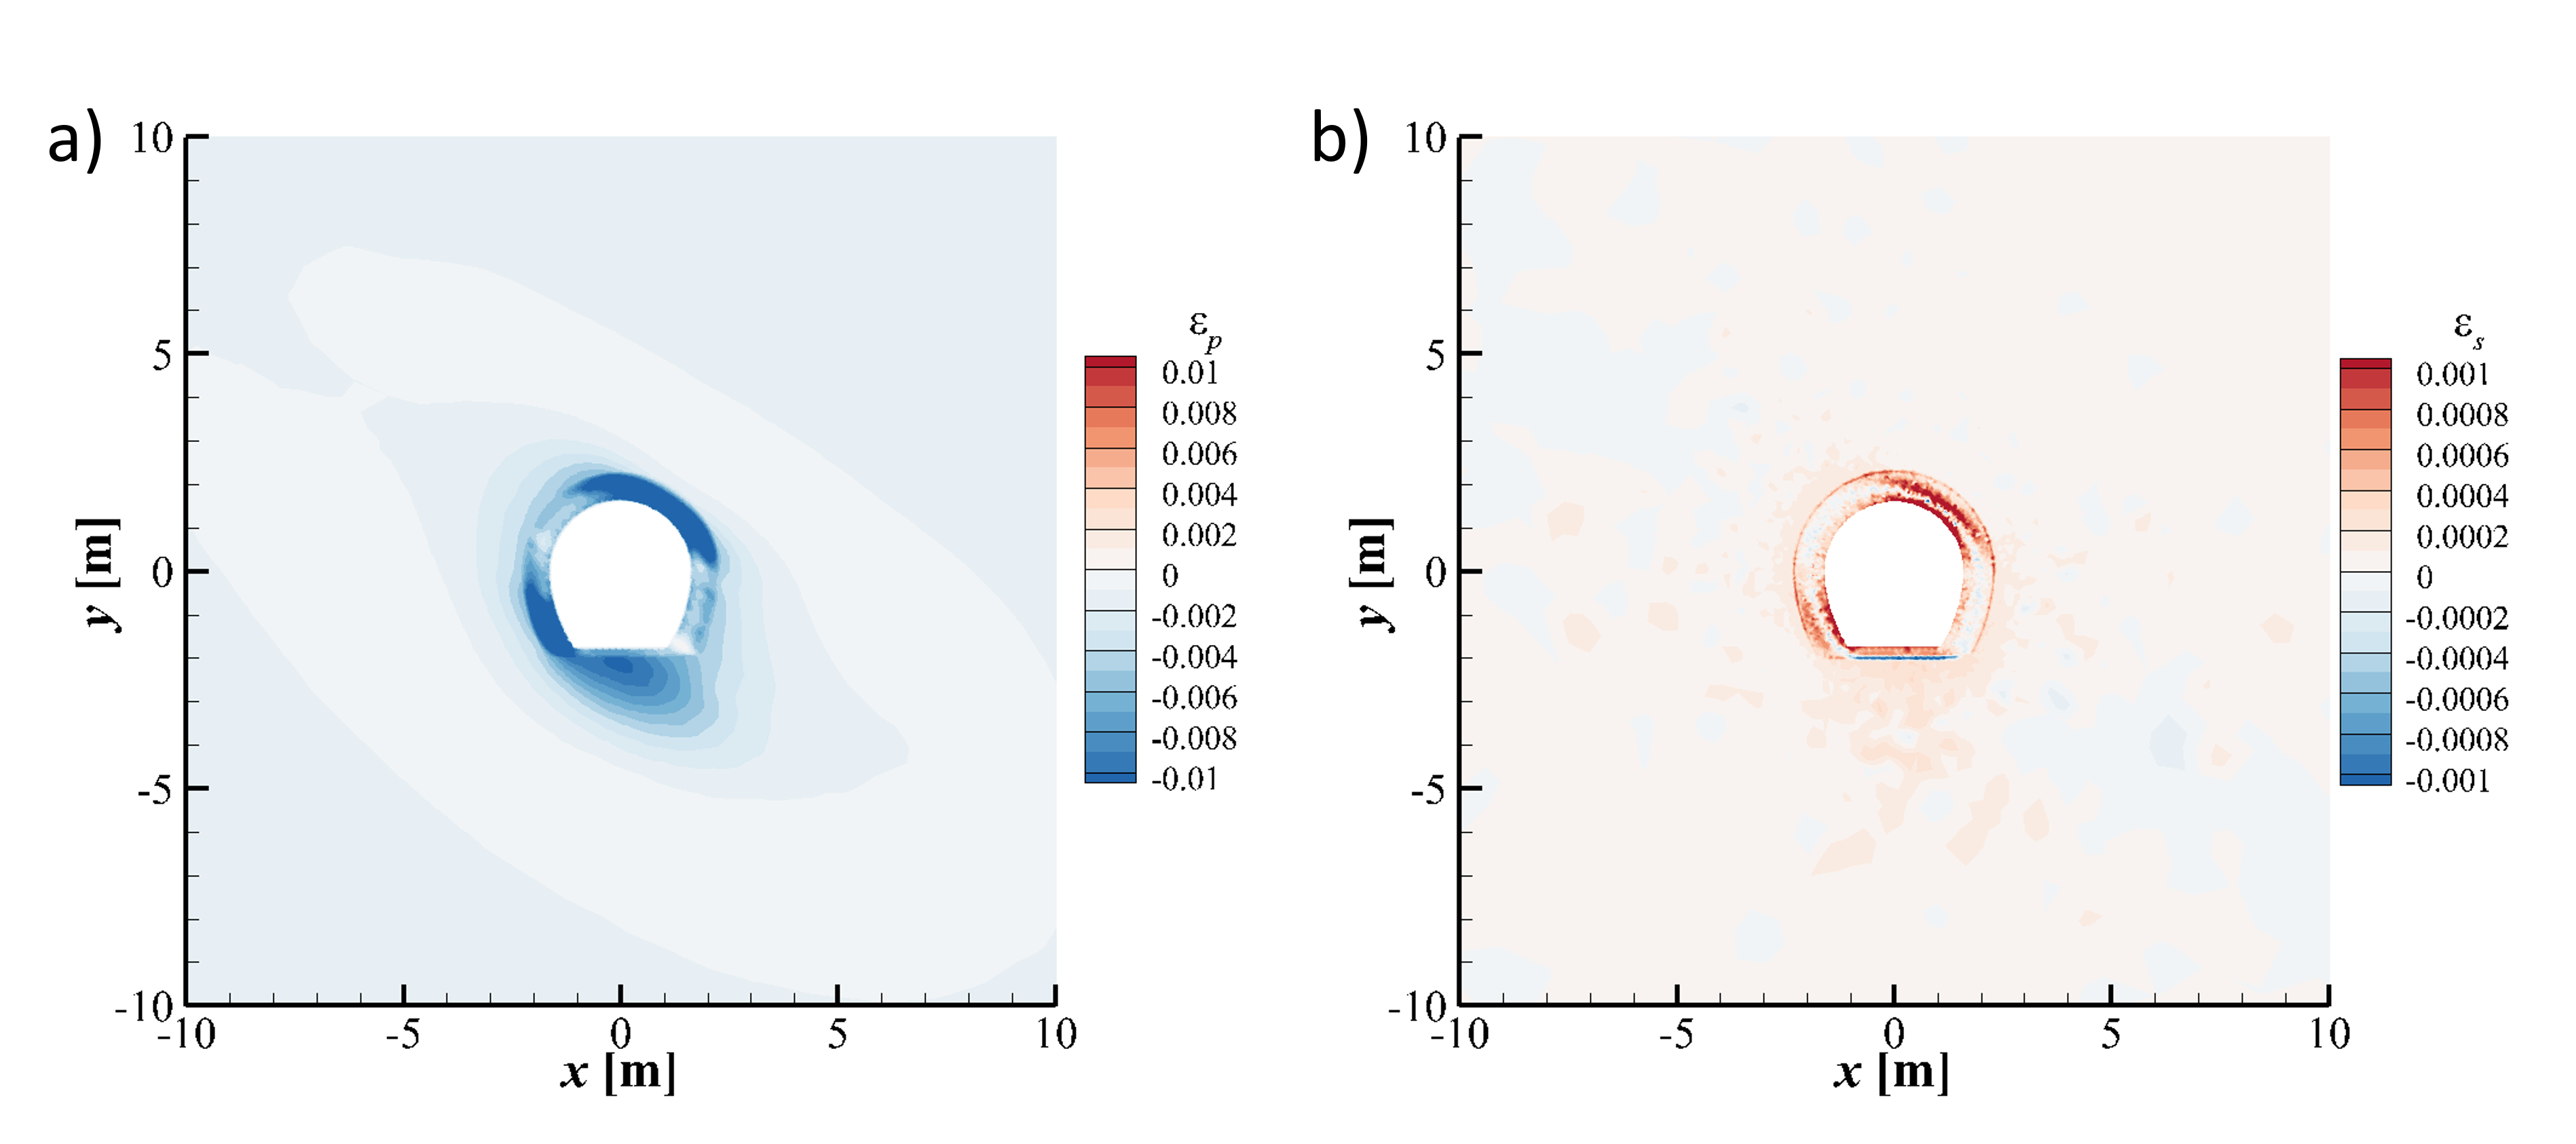
\includegraphics[width=\textwidth, trim=0.5cm  0.0cm 0 0.0cm, clip]{./figures/MEX10_cf_RF_RM_2d.png}
\caption{Deviation between 'Richards Flow' and 'Richards Mechanics' after 20 years of simulation time. a) Fluid pressure and b) effective saturation.}
\label{fig:richards_mechancis}
\end{figure}

The results of this comparison are shown in Figures \ref{fig:probe_RM_RF} and \ref{fig:richards_mechancis} as well as in Table \ref{tab:richards_mechanics}. For two sampling locations, the evolution of pressure and saturation show very good agreement. Note that the sampling locations for the data shown in Figure \ref{fig:probe_RM_RF} were taken inside the EDZ, since Figure \ref{fig:richards_mechancis} suggests that this is the area, where the strongest deviations can be expected. Indeed, while the cyclic saturation/desaturation is reproduced very well, there are differences in the maxima and minima between the two models for both quantities, $p_f$ and $S_\text{eff}$.  

Similar to the comparison made in Section \ref{sec:mex10_ogs5_vs_ogs6}, we define the simulation results reproduced by the RF model as the reference to compute the error
%
\begin{equation}\label{eq:error_rm_rf}
\epsilon_\theta = \frac{\theta^{RF}-\theta^{RM}}{\theta^{RF}}
\end{equation}
% 
as a quantitative estimate of the differences in the results of the two models. Looking at the two-dimensional deviations (Figure \ref{fig:richards_mechancis}), it becomes immediately obvious that pressure is slightly underestimated by the RM model in comparison with the RF model within the EDZ (which yields that saturation is overestimated). The differences between the results computed by the algorithms of the two models is one order of magnitude larger compared to the analysis performed in Section \ref{sec:mex10_ogs5_vs_ogs6}. Especially the pressure shows higher deviations (Figure \ref{fig:richards_mechancis}a) at the transition between the EDZ and the undisturbed rock and at the walls of the niche. Nevertheless, the results computed by the two models are overall very similar. The RMSE of the simulation results remains far below 1\% (Table \ref{tab:richards_mechanics}). Hence, the implementation of the Richards equation into the model "Richards Mechanics" can be accepted as trustworthy for the present scenario. 

\begin{table}
 \caption{Deviations observed when comparing 'Richards Flow' with 'Richards Mechanics' in OGS-6.\label{tab:richards_mechanics}}
\begin{center}
\begin{tabular}{ l | c | c | c }
 Quantity			& Minimum 	& Maximum	 & RMSE  \\
 \hline
 $p_f$ & -0.0505 	& 0.0055	& $8.56\cdot 10^{-4}$\\ 
 $S_\text{eff}$	 	& -0.0405 & 0.0112	& $2.66\cdot 10^{-3}$\\		
\end{tabular}
\end{center}
\end{table}


%%%%%%%%%%%%%%%%%%%%%%%%%%%%%%%%%%%%%%%%%%%%%%%%%%%%%%%%%%%%%%%%%%%%%%%%%%%%%%%%%%%%%%%%%
\subsubsection{Comparison of OGS-5 and OGS-6 for the full "Richards Mechanics"-model}\label{sec:full_RM}
%%%%%%%%%%%%%%%%%%%%%%%%%%%%%%%%%%%%%%%%%%%%%%%%%%%%%%%%%%%%%%%%%%%%%%%%%%%%%%%%%%%%%%%%%
For the analysis presented in this section, we use the exact same hydraulic model and the computational setup as described in Section \ref{sec:model_RF}. Furthermore, we parameterize the mechanical model, which was summarized in Section \ref{sec:model_RM} by choosing $\alpha=1.0$, and keep $K_f=K_s=1\cdot 10^{100}$ Pa to drive the storage term to zero. We define $\textbf{u}_0=0$ m, which is zero displacements for the initial conditions, and use roller boundary conditions at $x=-25$ m and $x=25$ m. We fix the domain at the bottom ($y=-25$ m) by defining $u_y\rvert_{y=-25\text{m}}=0$ m, but we leave the upper boundary to be completely frictionless in both, the $x$ and $y$ direction.

Finally, we need to parameterize the elasticity tensor $\mathds{C}$, which is a function of the Young's modulus $E$ and Poissons' ratio $\nu$, where, again, we distinguish between undisturbed rock ($E_1$) and the EDZ ($E_2$). The parameterization of $\mathds{C}$, however, is conceptually different for isotropic and transverse isotropic conditions, since one can use different definitions depending on the simplicity/symmetry of the problem. Since we are investigating both conditions, these definitions will be detailed below. The transverse isotropic condition is known to be more adequate for clayrock owing to the bedding of this particular rock and it was also used in the study of \cite{ziefle2018}.

\subsubsection*{Isotropic elasticity}
As mentioned above, we use the Voigt notation to write the three-dimensional elasticity tensor. For isotropic conditions, $\mathds{C}$ simplifies from the general form to
\begin{equation}
\mathds{C} =  \frac{E}{(1+\nu)(1-2\nu)}	
				\begin{pmatrix}
				1-\nu 	& \nu	& \nu	& 0				   &0					&0 	\\
				\nu	  	& 1-\nu	& \nu	& 0				   &0					&0	\\
				\nu		& \nu	& 1-\nu	& 0				   &0					&0	\\		
				0		& 0		& 0		& \frac{1-2\nu}{2} &0					&0	\\		
				0		& 0		& 0		&0				   &\frac{1-2\nu}{2}	&0	\\		
				0		& 0		& 0		&0				   &0      &\frac{1-2\nu}{2}
				\end {pmatrix}
\end{equation}
Hence, $\mathds{C}$ is fully parameterized with $\nu=0.18$ for both material groups, $E_1=3.6 \times 10^9$ Pa for the undisturbed rock and $E_2=1.8\times 10^9 $ Pa for the EDZ.


While the simulation results of the RM-model yield very similar spatial distributions of $p_f$ and $S_\text{eff}$ that were reported in Figure \ref{fig:results}, we know obtain values for the deformation vector $\textbf{u}$. The results for the two components after a simulation time of 20 years is shown in Figure \ref{fig:RM_displacement_isotropic}. The overall impact of the saturation/desaturation on the mechanical behavior is such that the tunnel is compressed in its height, whereas the lateral distance between the walls increases. This deformation leads to a compression in the undisturbed rock farther away from the niche.  

\begin{figure}[t]
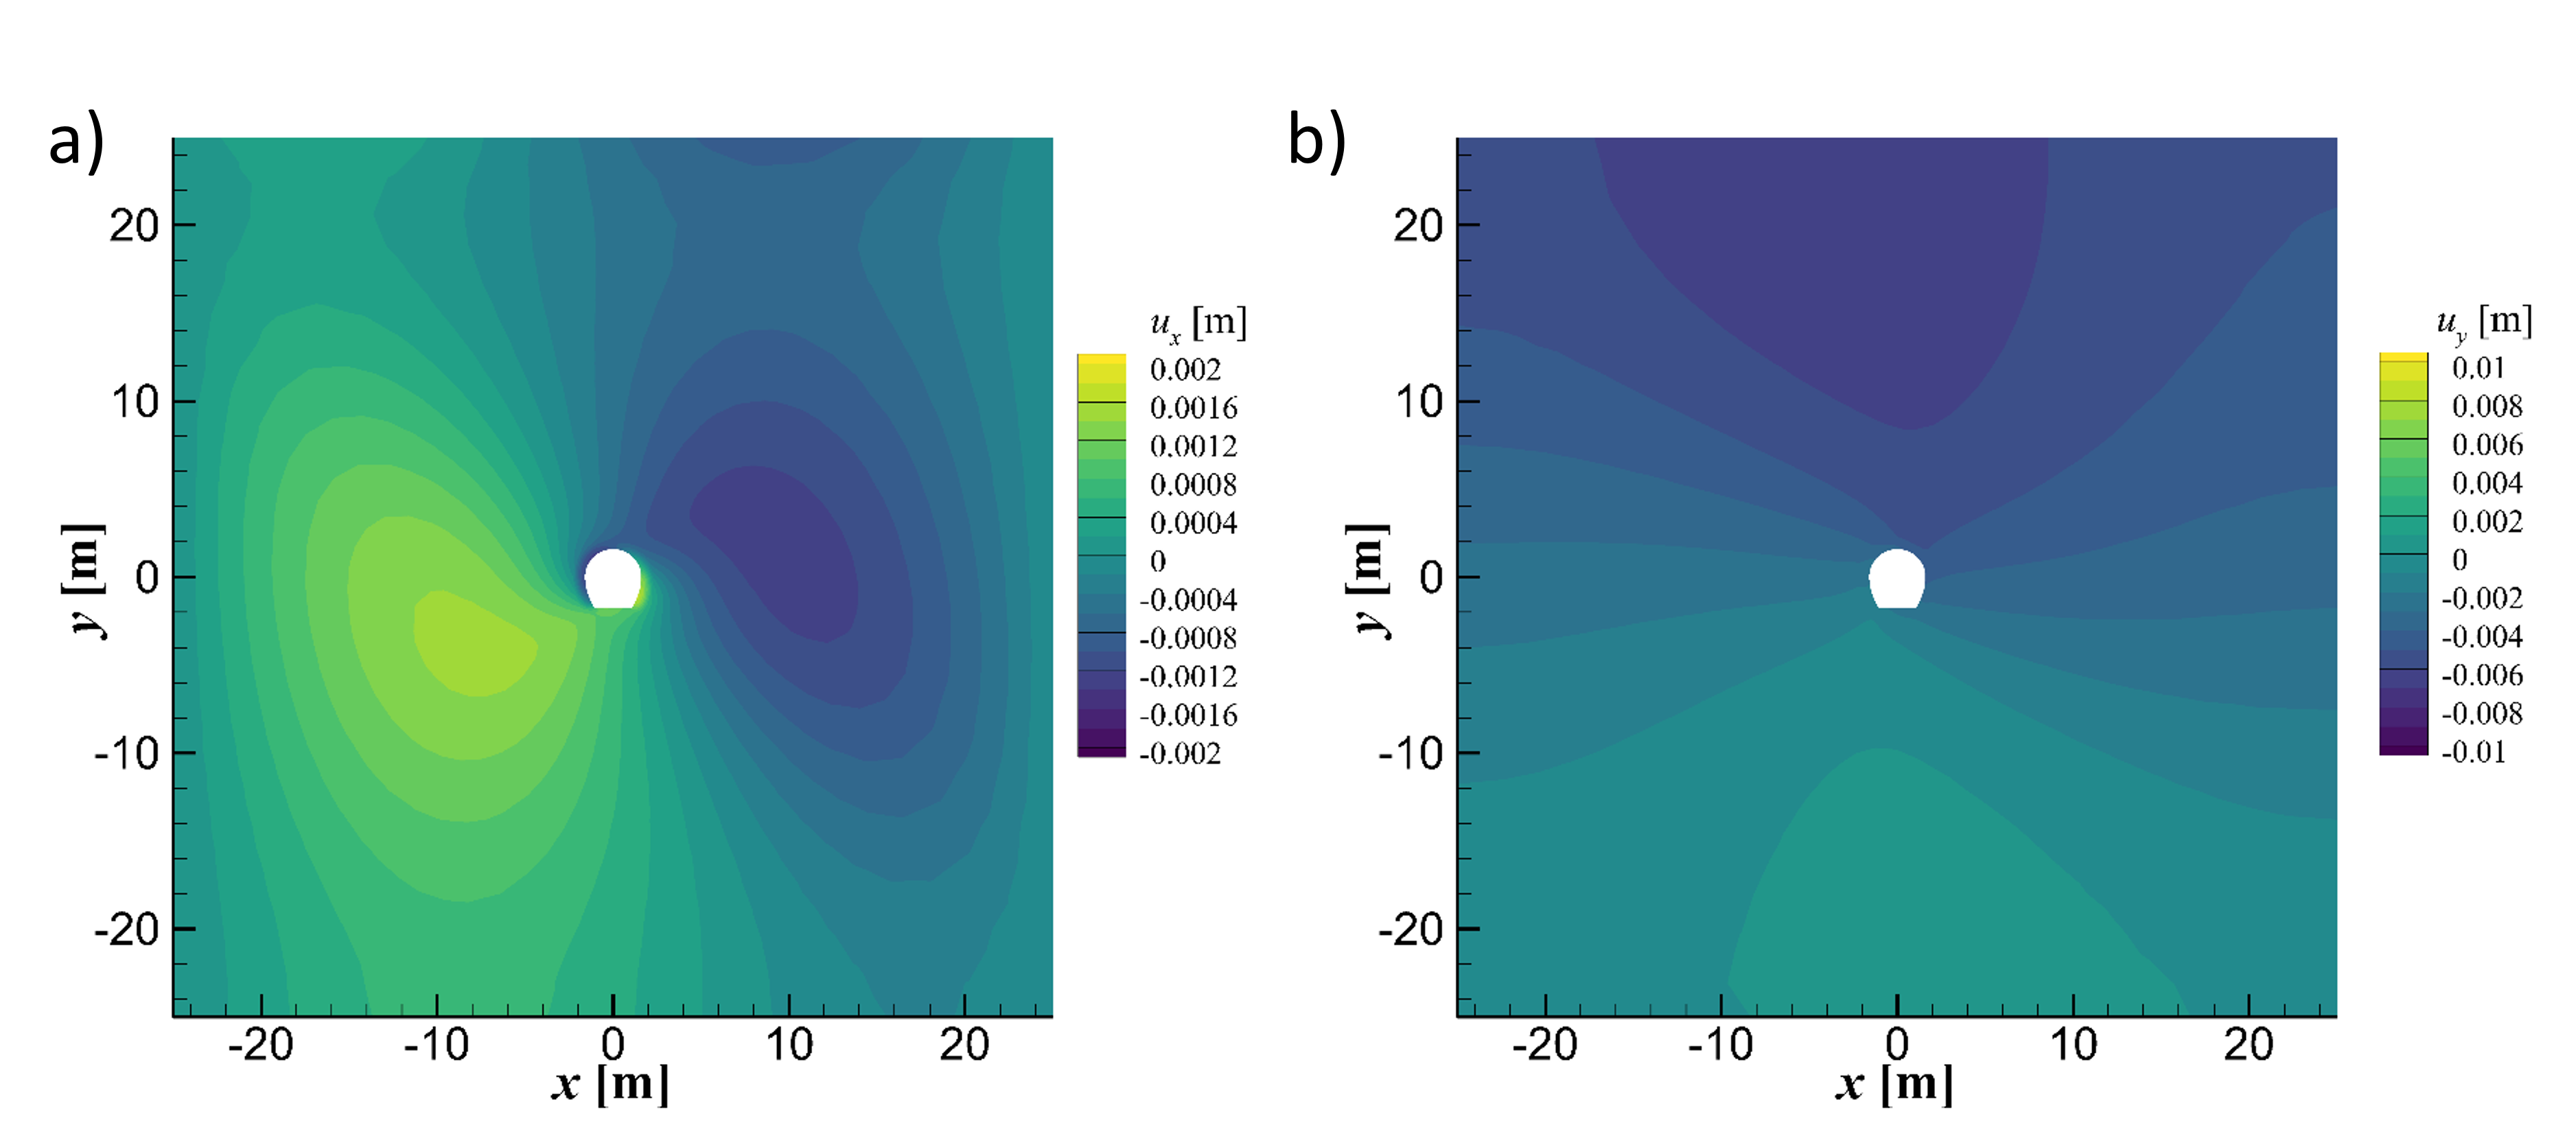
\includegraphics[width=\textwidth, trim=0.5cm  0.0cm 0 0.0cm, clip]{./figures/MEX10_RM_OGS5_isotropic.png}
\caption{Spatial distribution of the rock deformation $\textbf{u}$  for isotropic conditions after 20 years of simulation time. a) horizontal deformation $u_x$ and b) vertical deformation $u_y$.}
\label{fig:RM_displacement_isotropic}
\end{figure}

\begin{figure}[t]
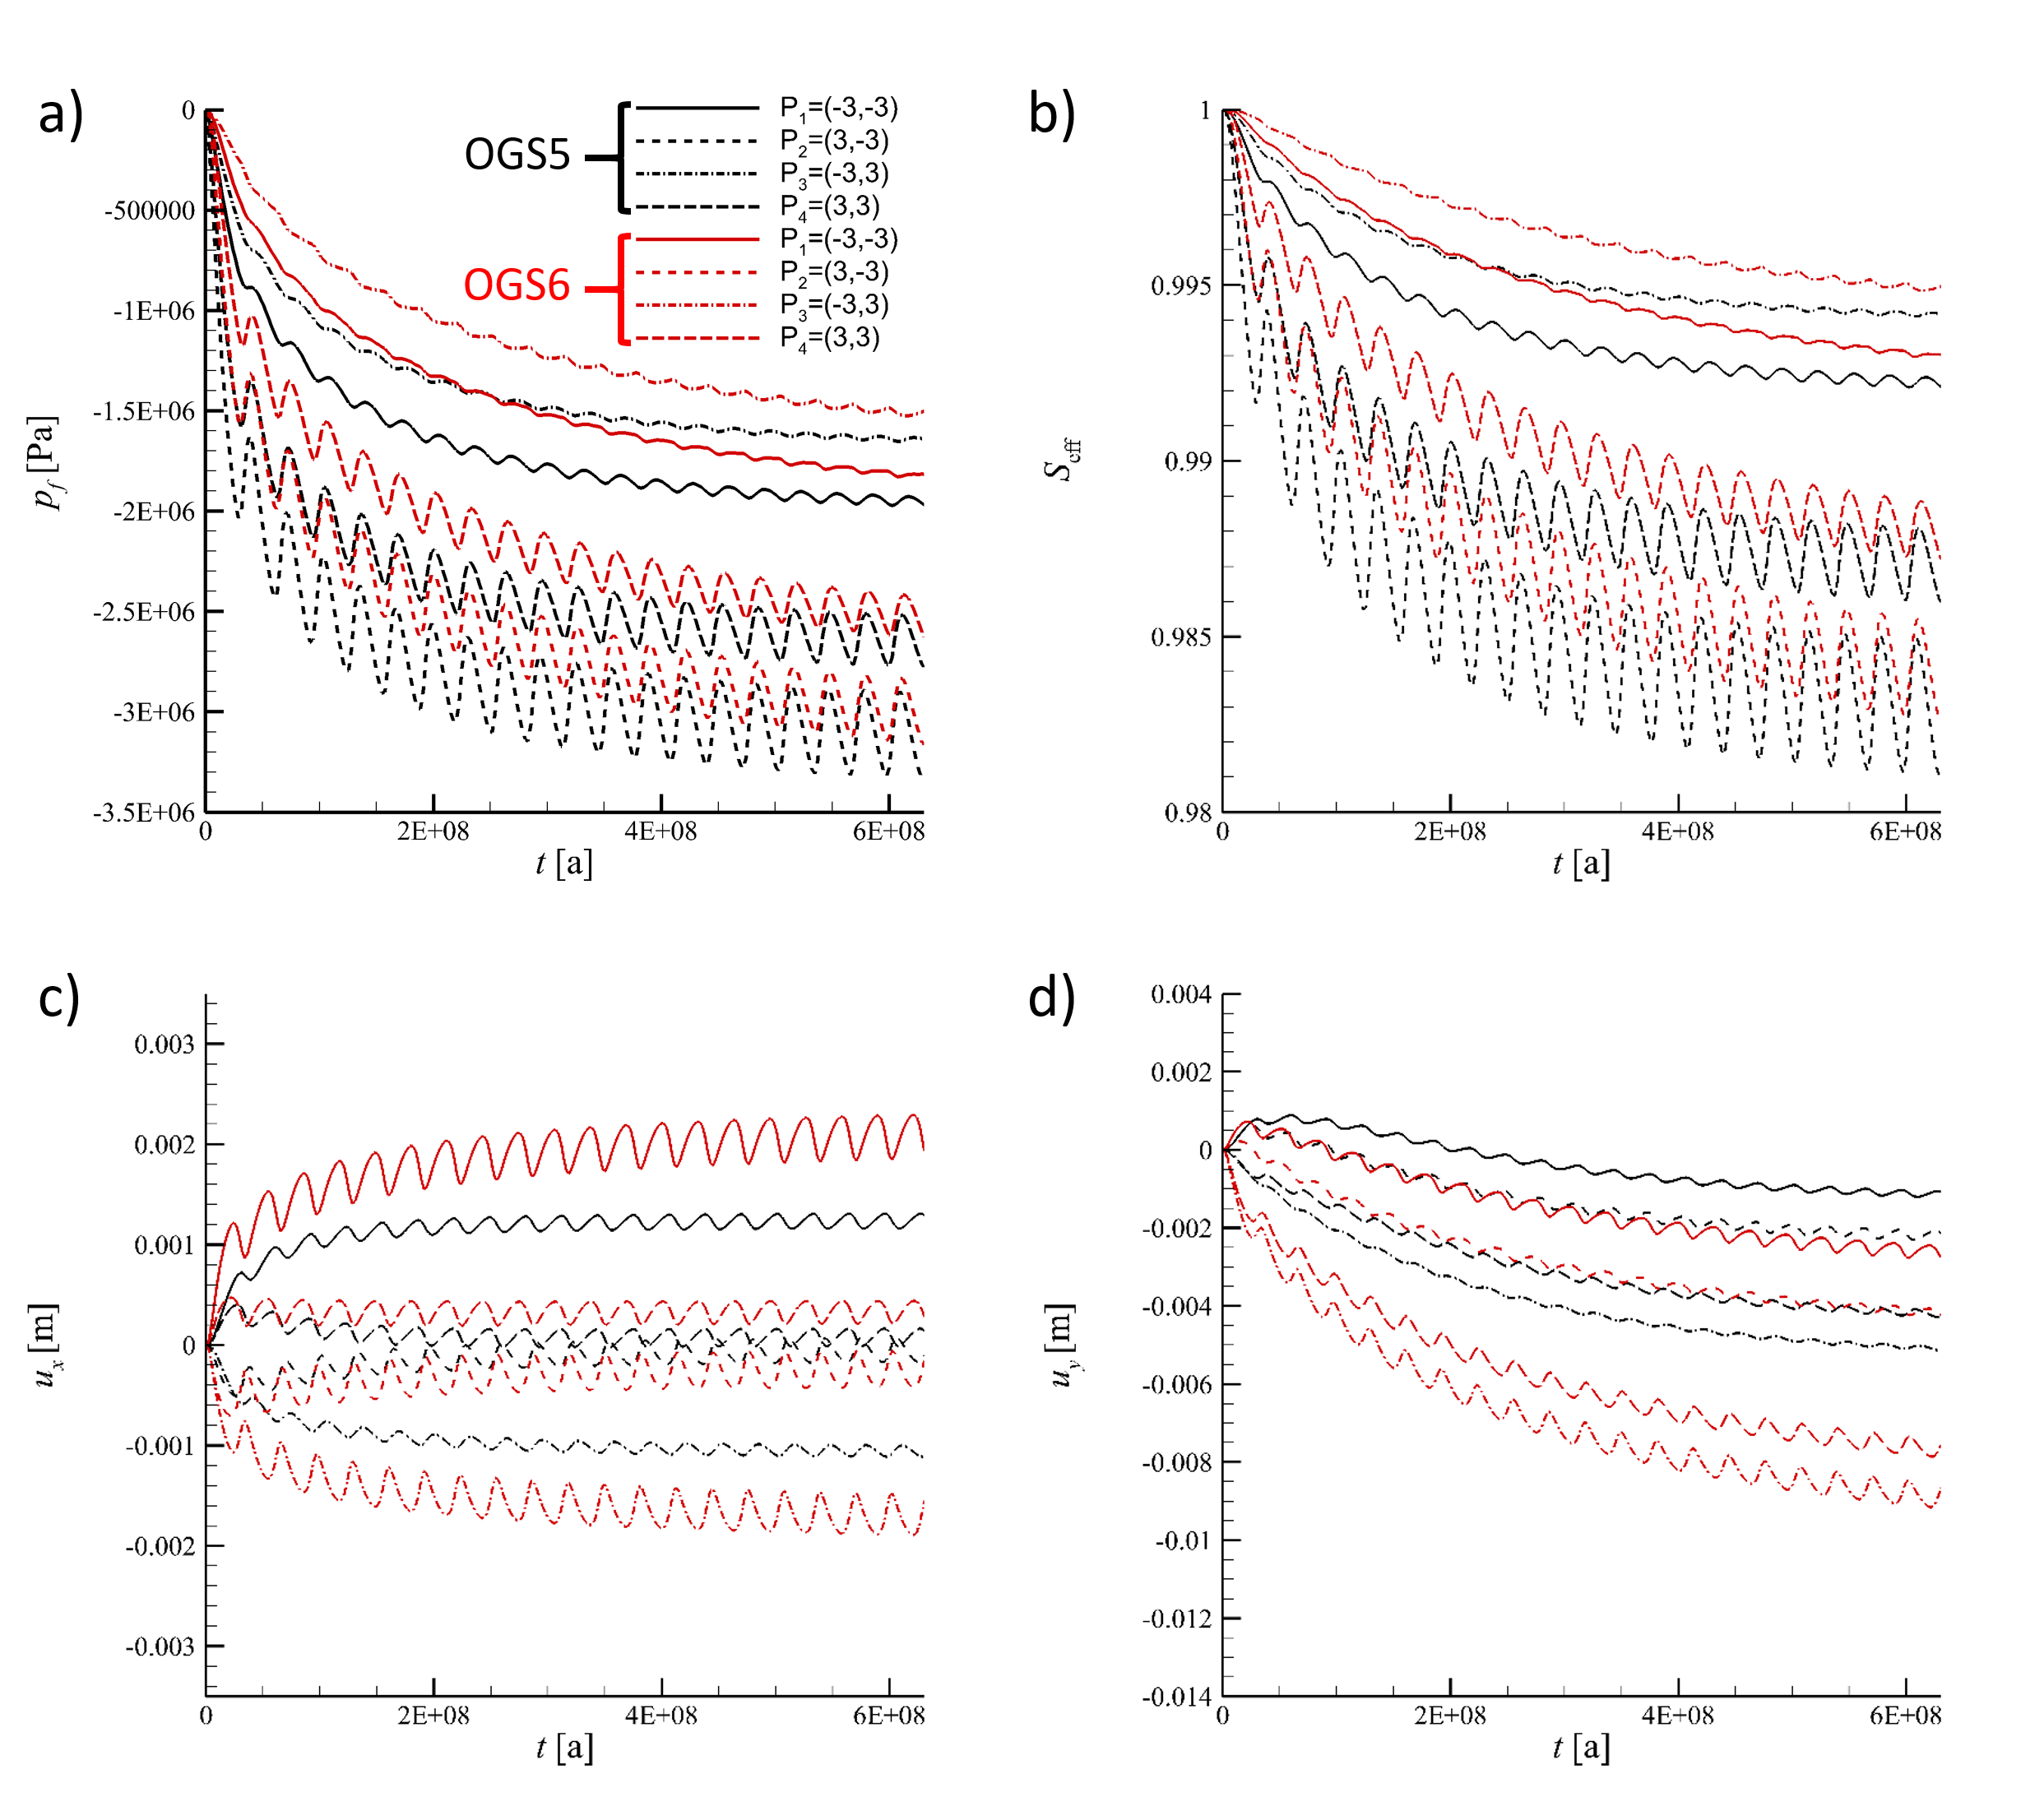
\includegraphics[width=\textwidth, trim=0.5cm  0.0cm 0 0.0cm, clip]{./figures/MEX10_probe_over_time_isotropic.png}
\caption{Physical quantities computed by OGS-5 and OGS-6 for isotropic conditions probed over time at the same four locations depicted in the inset of Figure \ref{fig:cf_P_S}. a) Fluid pressure, b) effective saturation, c) horizontal deformation and d) vertical deformation.}
\label{fig:RM_probe_over_time_isotropic}
\end{figure}

To compare the simulation results of the two FE codes OGS-5 and OGS-6, we probe the generated data of $p_f$, $S_\text{eff}$, $u_x$ and $u_y$ over time at the sampling points illustrated in the inset of Figure \ref{fig:cf_P_S}. Unlike the very good agreement obtained in that figure, we now find significant deviations between the simulation results of OGS-5 and OGS-6. This is true for all physical quantities at all sampling points. We obtain a systematically higher pressure and, hence, a higher saturation for OGS-6. This difference also causes different mechanical deformations of the rock, but these quantities do not differ as systematic as the pressure does. The difference can be explained by the different coupling schemes of the two codes. While OGS-5 uses a staggered scheme with a weak coupling of the two processes, OGS-6 provides a monolithic scheme that allows for a strong coupling of the hydraulic and mechanical processes by solving for $p_f$ and $\textbf{u}$ simultaneously. The strongly coupled monolithic scheme is known to yield better results than the weakly coupled staggered scheme \cite{hubner2003,farhat2000}. Hence, the simulation results generated by OGS-6 potentially provide more realistic results than OGS-5 does. However, a detailed comparison to analytic reference solutions or experimental benchmark data will be needed to verify this hypothesis.


Despite the differences of the results reported in Figure \ref{fig:RM_probe_over_time_isotropic}, both simulations yield qualitatively the same results, albeit with different magnitudes in deformation. This becomes evident in the spatial distribution of the error \eqref{eq:error}, which is shown in Figure \ref{fig:RM_error_2d_isotropic}. Note that values of $\epsilon_{u,x}$ and $\epsilon_{u,y}$ were normalized by the width of the niche, which is 3.2 m, rather than $\epsilon^{OGS5}$, as normalizing by the small deformation values is prone to indicate unreasonably large errors. Even though there is a direct dependency of effective saturation on fluid pressure, the spatial distributions of the relative error for these two quantities look very differently (Figure \ref{fig:RM_error_2d_isotropic}a and b). The rather large error for fluid pressure especially far away from the niche can be attributed to low values of $p_f$ that are used to normalize \eqref{eq:error_rm_rf}. Closer to the niche, the error decays to smaller values. Looking at the spatial distribution of the error for all other quantities, however, we can conclude that even though the coupling scheme of OGS-6 is more powerful than the scheme of OGS-5, both simulations yield similar results. This fact is also reflect in the maxima, minima and RMSE \eqref{eq:RMSE}. Even though the deviations in pressure are rather large, the overall change in deformation with respect to the characteristic length of the problem, i.e. the width of the niche, remains small. Nevertheless, unlike the comparison presented in Section \ref{sec:model_RF}, we observe substantial deviations for the simulation results from OGS-6 compared to those generated using OGS-5. Further research will be needed to clarify these differences. 

\begin{figure}[t]
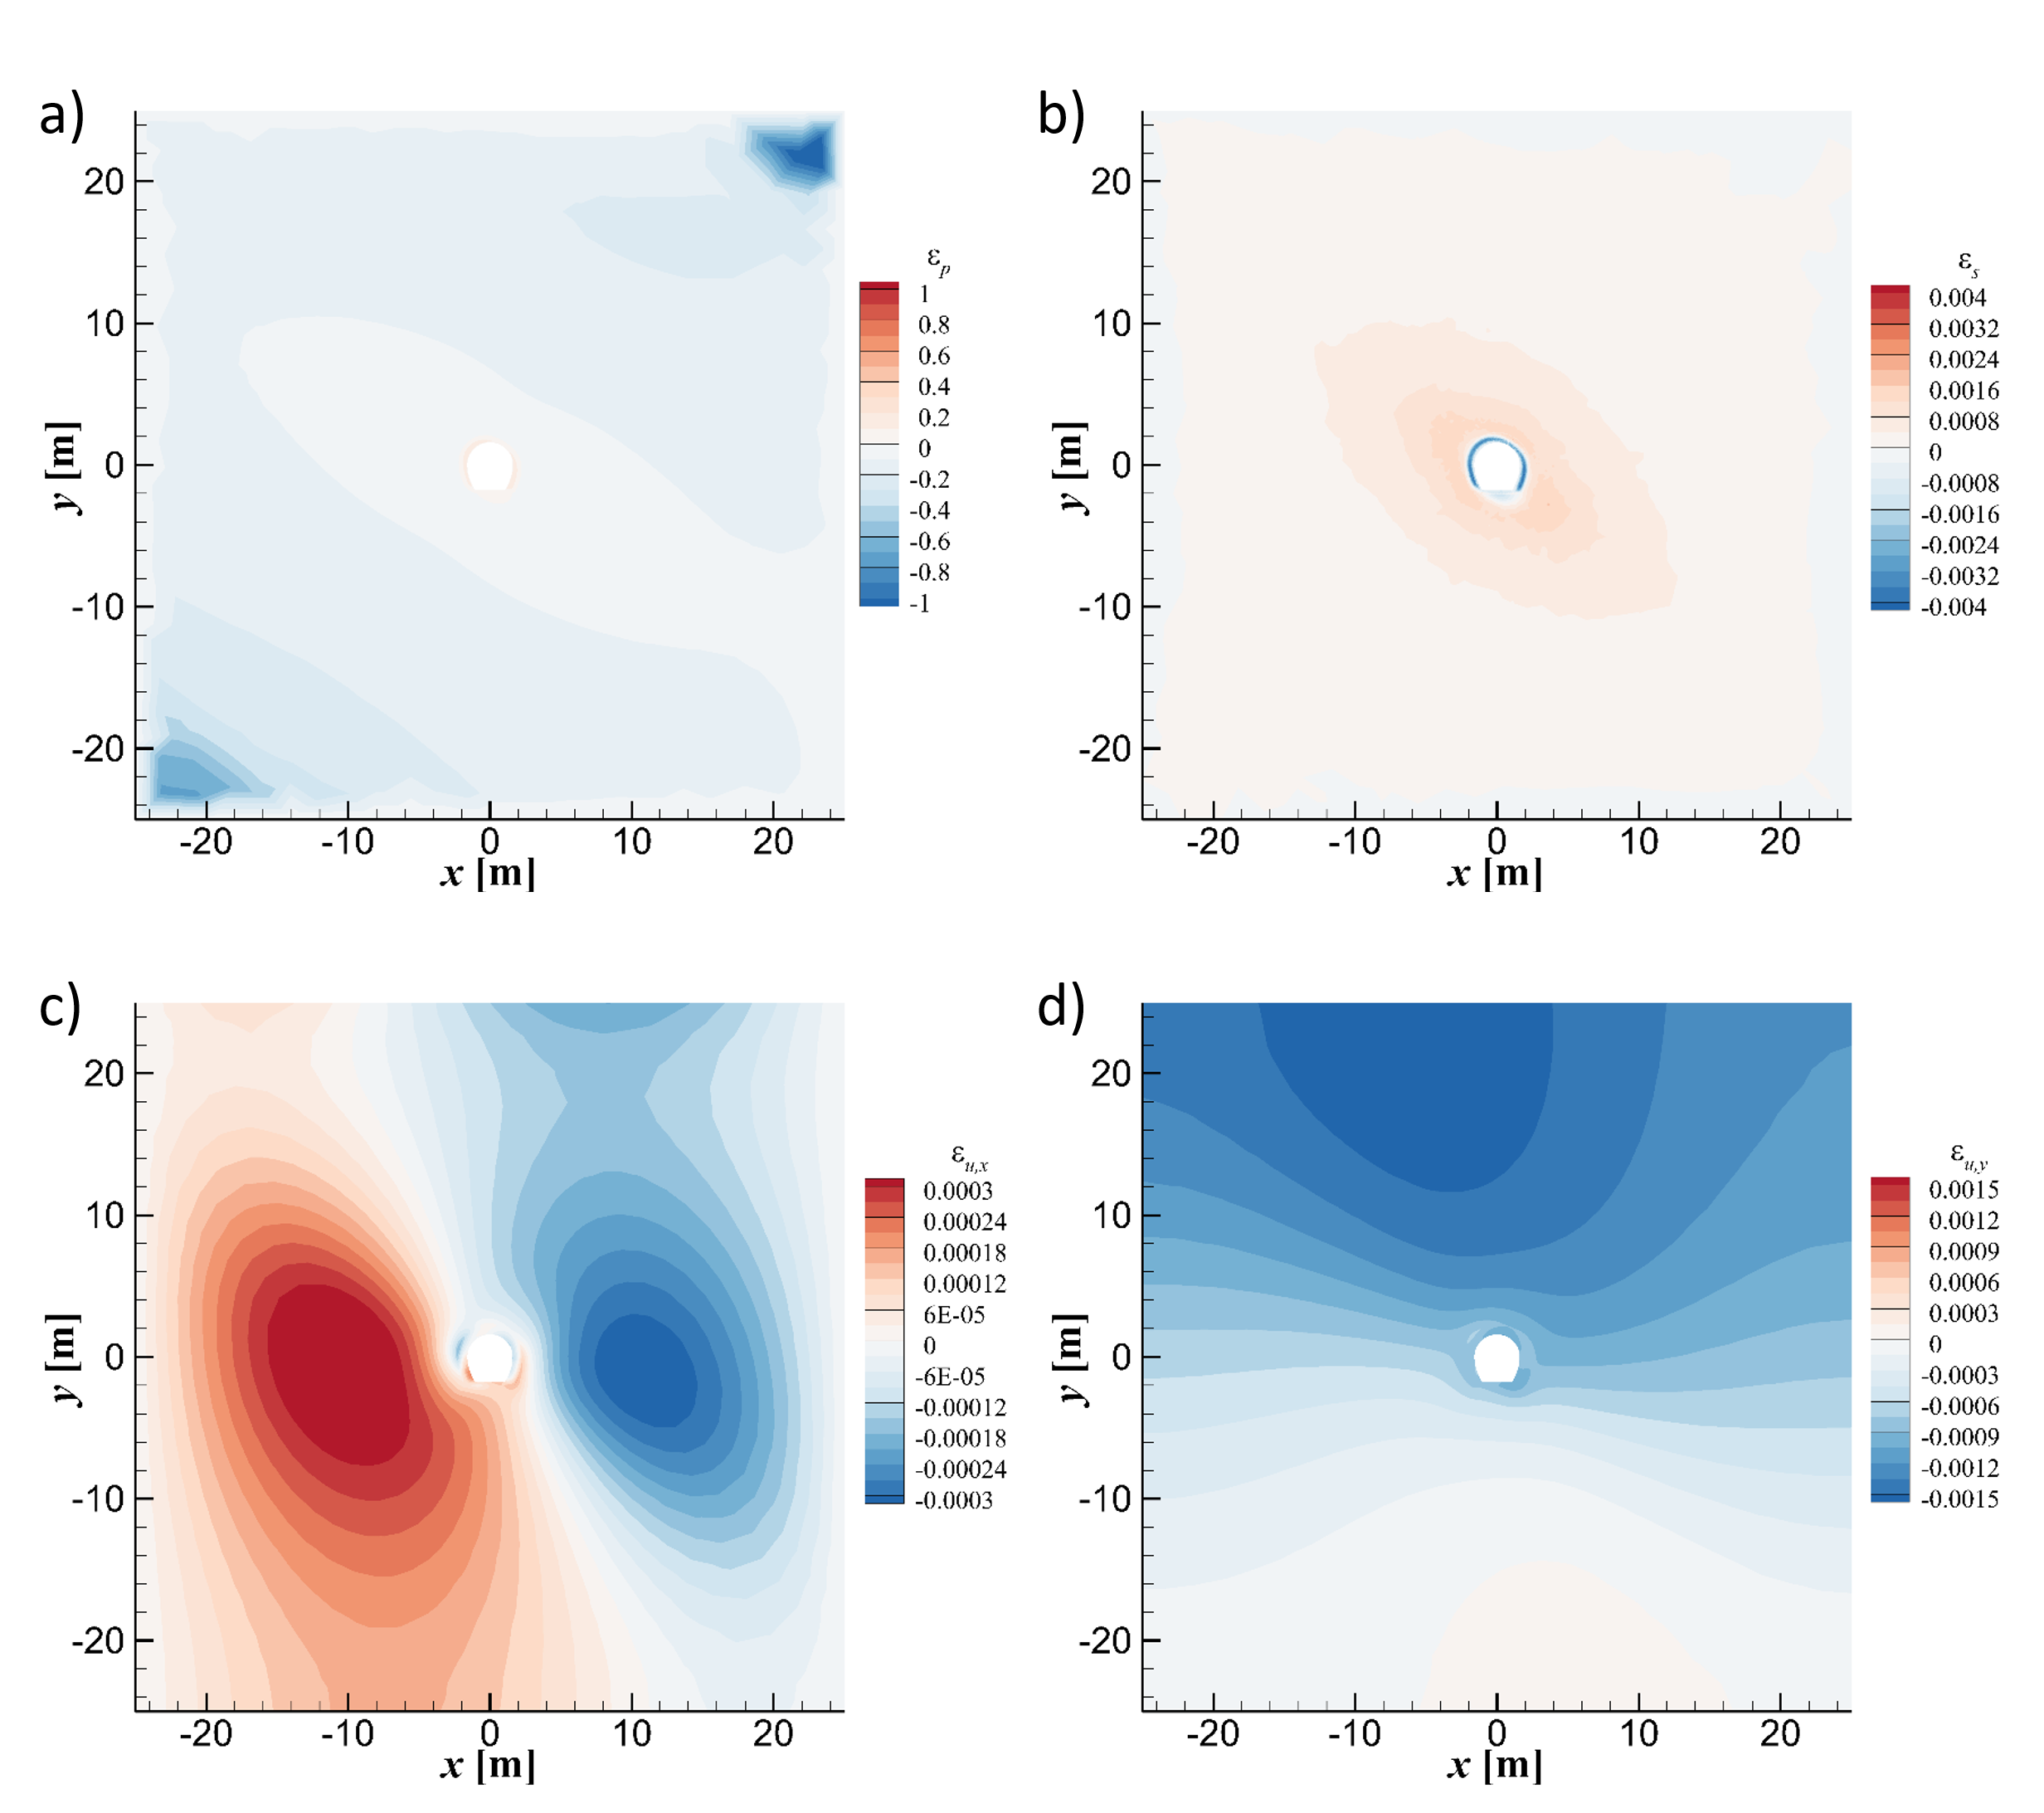
\includegraphics[width=\textwidth, trim=0.5cm  0.0cm 0 0.0cm, clip]{./figures/MEX10_RM_error_2d_isotropic.png}
\caption{Deviations between OGS-5 and OGS-6 for isotropic conditions after 20 years of simulation time.  a) Fluid pressure, b) effective saturation, c) horizontal deformation and d) vertical deformation.}
\label{fig:RM_error_2d_isotropic}
\end{figure}

\begin{table}
 \caption{Deviations observed when comparing OGS-5 with OGS-6 for the RM model with isotropic conditions.\label{tab:error_RM_isotropic}}
\begin{center}
\begin{tabular}{ l | c | c | c }
 Quantity				& $\min{(\epsilon)}$ 	& $\max{(\epsilon)}$	 & RMSE  \\
 \hline
 $p_f$				& -1.1514 				& 0.1478 			& $6.81\cdot 10^{-2}$\\ 
 $S_\text{eff}$	 	& -0.0045 				& 0.0017			& $1.12\cdot 10^{-3}$\\		
 $u_x$				& -0.0003 				& 0.0004			& $8.97\cdot 10^{-5}$\\		 
 $u_y$			 	& -0.0016 				& $3\cdot10^{-5}$	& $8.44\cdot 10^{-4}$\\	
\end{tabular}
\end{center}
\end{table}

\subsubsection*{Anisotropic elasticity}
We consider the transverse isotropic behavior of clayrock described in Section \ref{sec:model_RF} by defining a higher stiffness parallel to the bedding $E_i$ and a lower stiffness normal to the bedding $E_a$. Here, the subscripts $i$ and $a$ indicate directions parallel and perpendicular to the bedding plane, respectively. Similarly, the Poisson's ratio has to be defined with respect to the anisotropy  direction that is normal to the bedding $\nu_{ia}$ and parallel to the bedding $\nu_{ii}$.  The inverse of the elasticity tensor then becomes
\begin{equation}
\mathds{C}^{-1} =  	\begin{pmatrix}
 	\frac{1}{E_i} 		& -\frac{\nu_{ai}}{E_a}	& -\frac{\nu_{ii}}{E_i}	& 0	&0	&0 	\\
	-\frac{\nu_{ia}}{E_i}&\frac{1}{E_a}			& -\frac{\nu_{ia}}{E_a}	& 0	&0	&0 	\\
	-\frac{\nu_{ii}}{E_i}& -\frac{\nu_{ai}}{E_a}	&\frac{1}{E_i}		& 0	&0	&0 	\\
				0		& 0		& 0		& \frac{1}{G_a} &0				&0			\\		
				0		& 0		& 0		&0				&\frac{1}{G_i}	&0			\\	
				0		& 0		& 0		&0				&0		      	&\frac{1}{G_a} 	
				\end {pmatrix}
\end{equation}
where $G_i=E_i/(2+2\nu_{ii})$ and $G_a$ are the shear moduli in isotropic and anisotropic direction, respectively. Note that the elasticity tensor is not symmetric. Instead, we need to rescale $\nu_{ai}=\nu_{ia} \frac{E_a}{E_i}$. Here, we have used the same values as \cite{ziefle2018}, which were $E_{i}=3.6\times10^9$ Pa, $E_{a}=1.1\times10^9$ Pa, $\nu_{ia}=0.16$ and $\nu_{ii}=0.18$ and  $G_a=1.2\times10^9$ Pa. We rotate the elasticity tensor by the same angle of inclination $\gamma = -32.96^{\circ}$ that was applied to the permeability tensor \eqref{eq:permeabilities}. 

\begin{figure}[t]
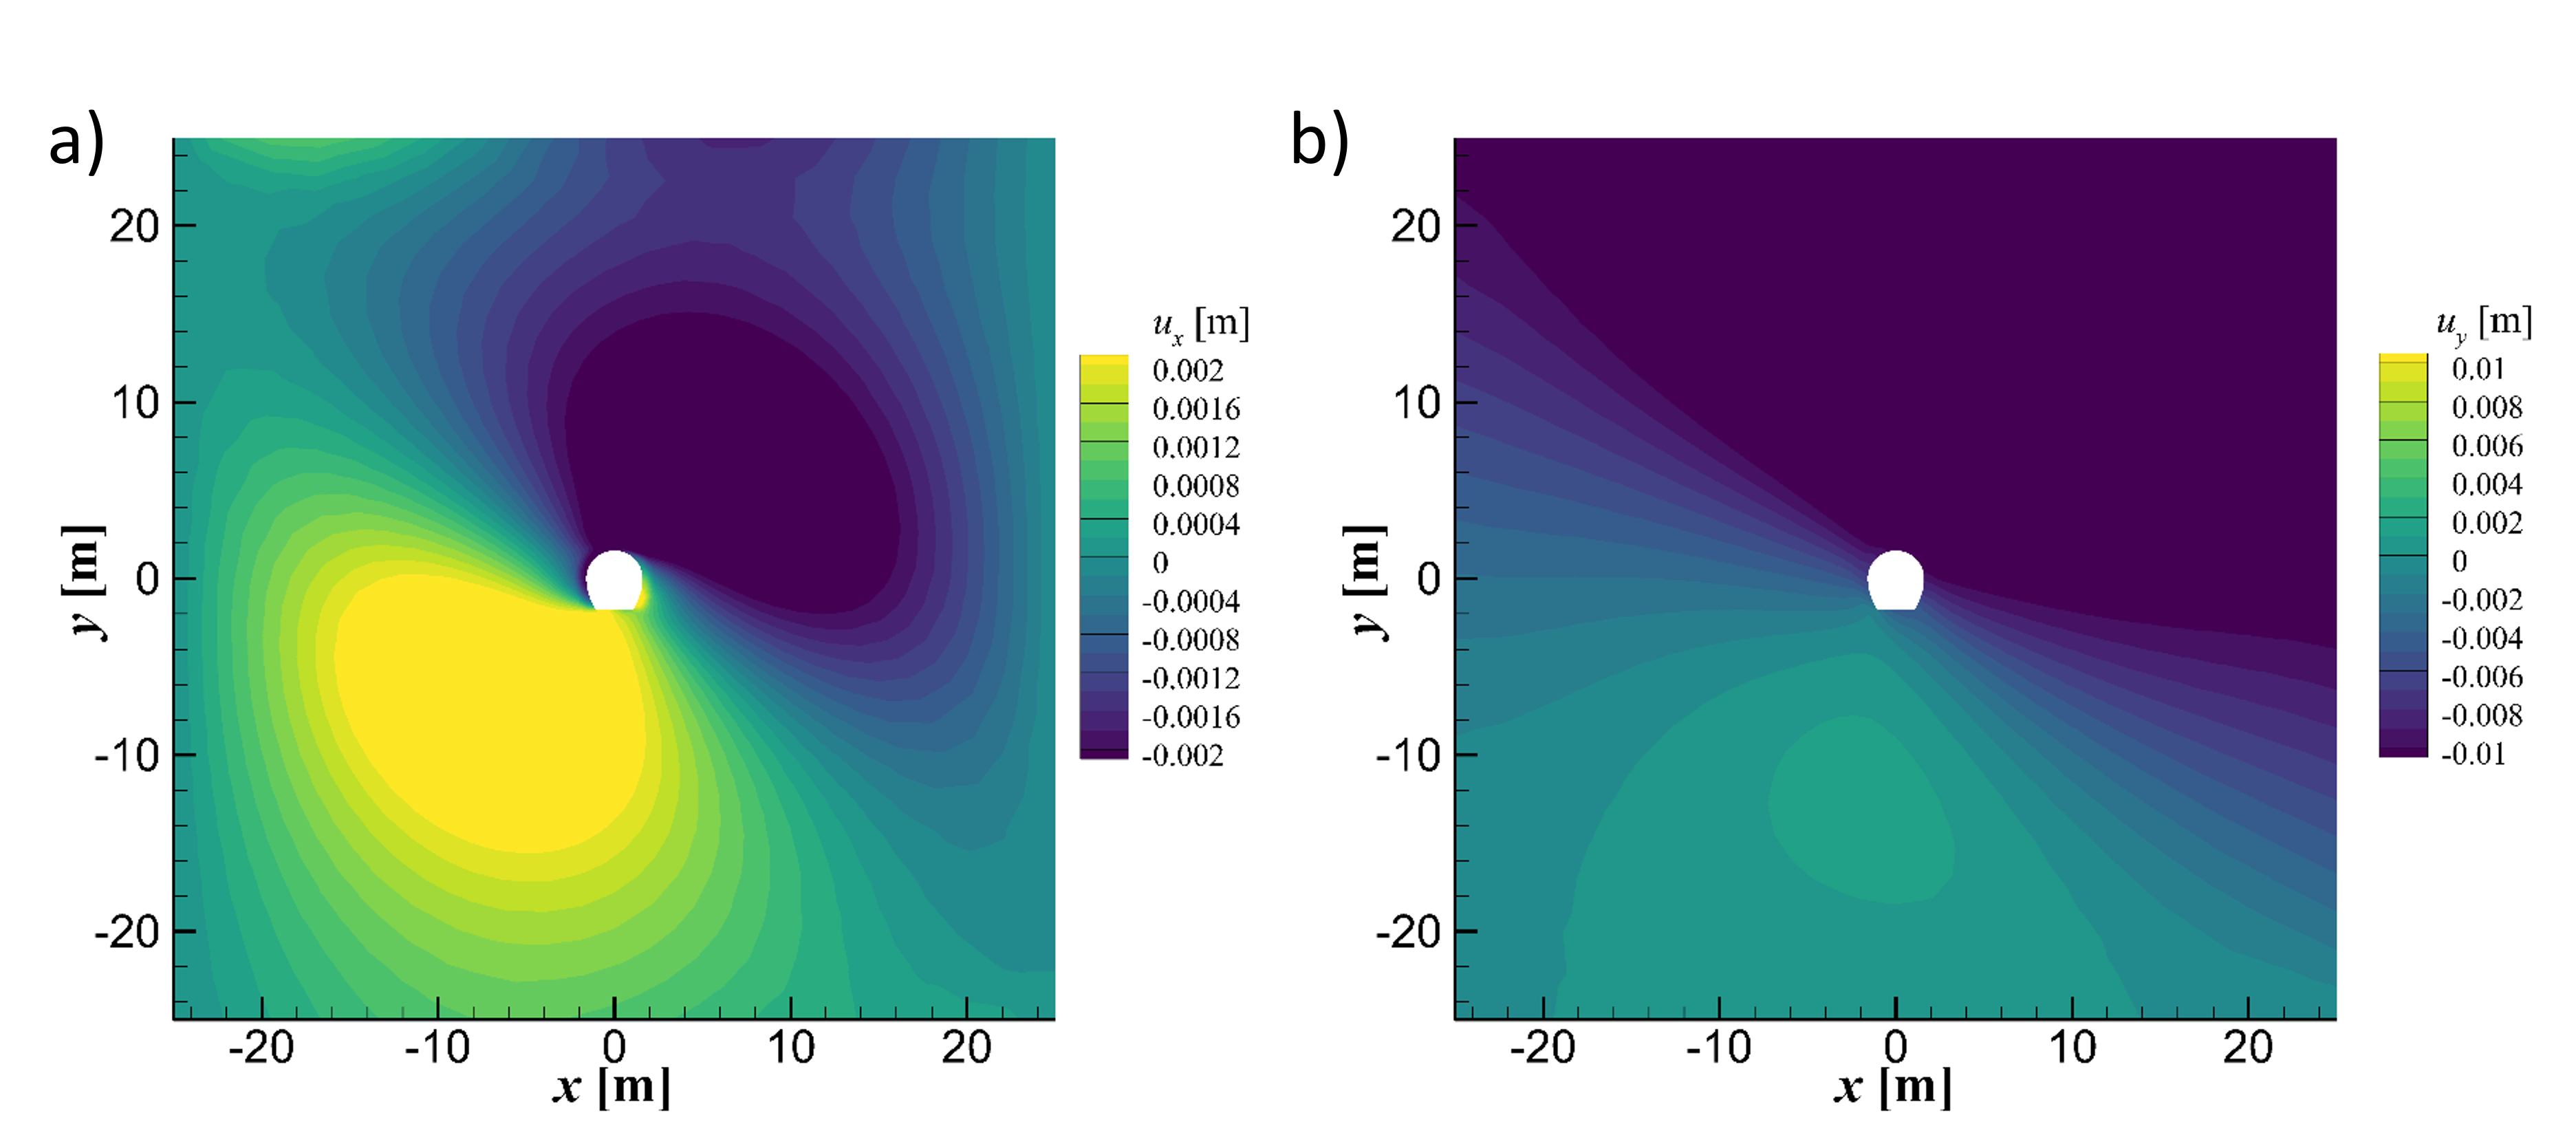
\includegraphics[width=\textwidth, trim=0.5cm  0.0cm 0 0.0cm, clip]{./figures/MEX10_RM_OGS5_anisotropic.png}
\caption{Spatial distribution of the rock deformation $\textbf{u}$  for anisotropic conditions after 20 years of simulation time. a) horizontal deformation $u_x$ and b) vertical deformation $u_y$.}
\label{fig:RM_displacement_anisotropic}
\end{figure}

To illustrate the well-developed stage and to provide a comparison to the isotropic elasticity shown in Figure \ref{fig:RM_displacement_isotropic}, we plot the spatial distribution of the two components of the deformation in Figure \ref{fig:RM_displacement_anisotropic}. As desired,the maximum and minimum horizontal deformations have rotated for the anisotropic case according to the angle of inclination. Other than that, the simulation results of the isotropic and anisotropic case  remain very similar.

\begin{figure}[t]
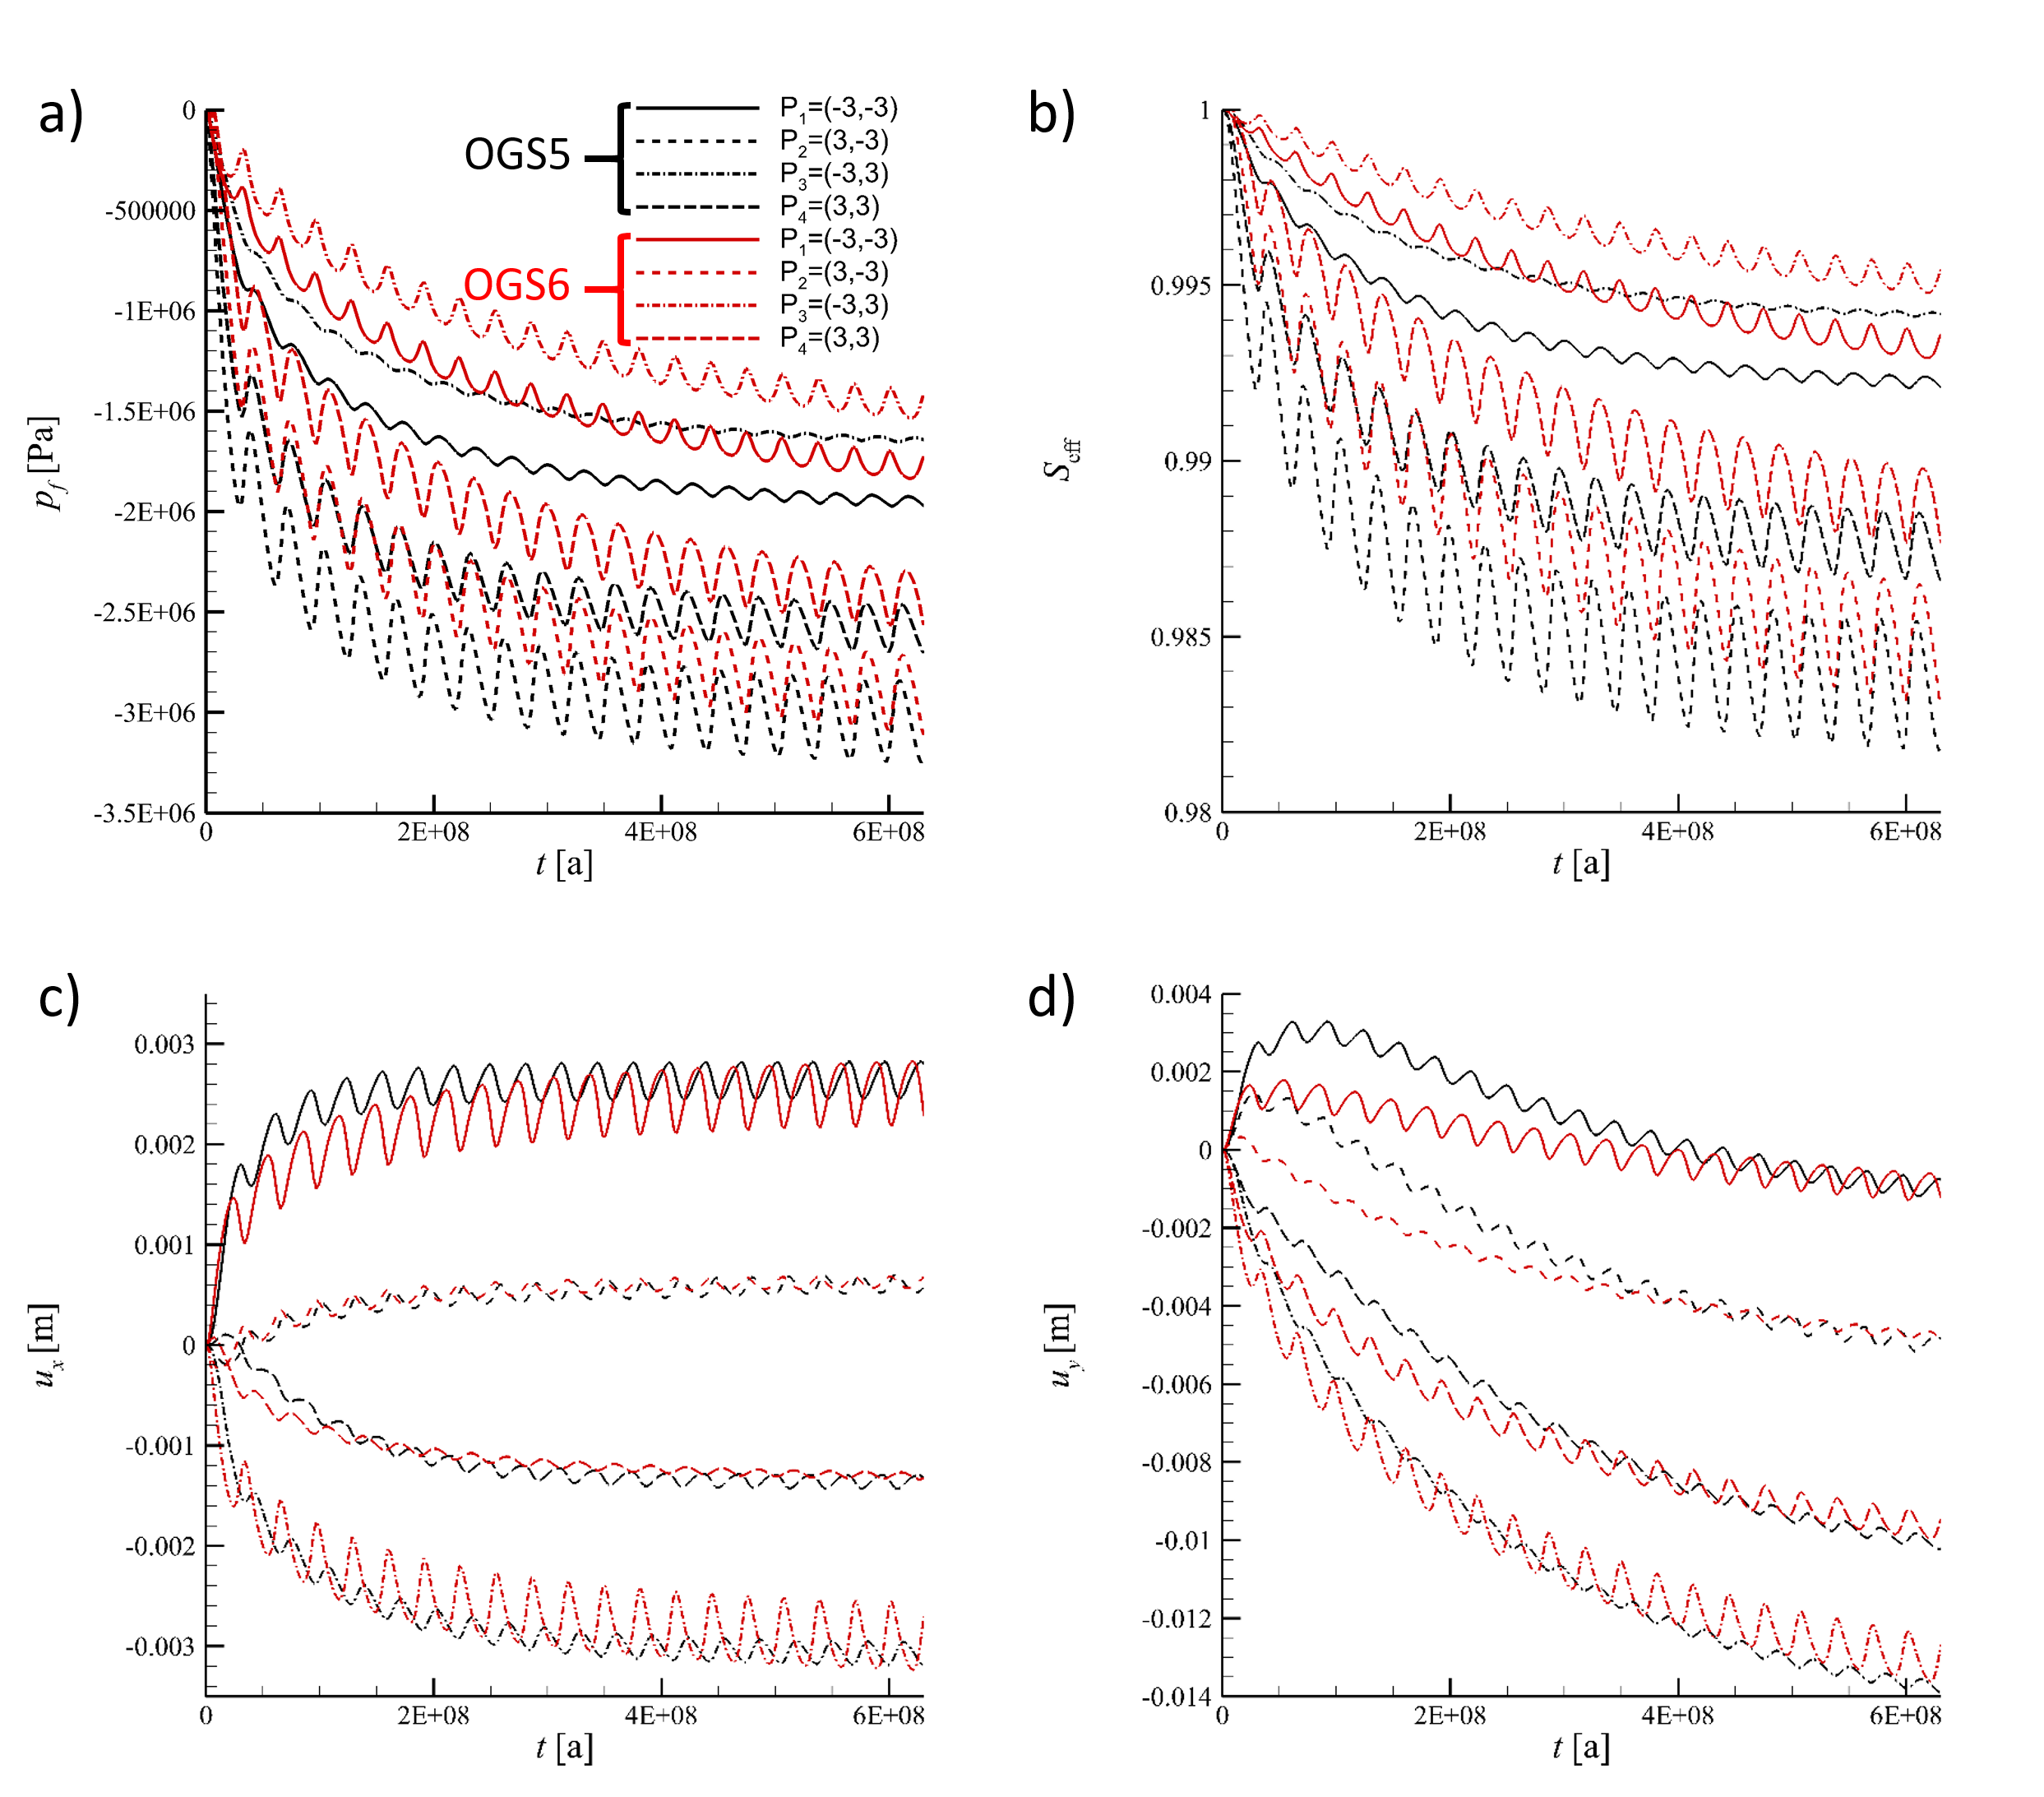
\includegraphics[width=\textwidth, trim=0.5cm  0.0cm 0 0.0cm, clip]{./figures/MEX10_probe_over_time_anisotropic.png}
\caption{Physical quantities computed by OGS-5 and OGS-6 for anisotropic conditions probed over time at the same four locations depicted in the inset of Figure \ref{fig:cf_P_S}. a) Fluid pressure, b) effective saturation, c) horizontal deformation and d) vertical deformation.}
\label{fig:RM_probe_over_time_anisotropic}
\end{figure}

The similarity between the isotropic and the anisotropic behavior yield the same results for the pointwise sampling of physical quantities over time. Values for fluid pressure and effective saturation are systematically higher for OGS-6. However, the deviations of the deformation  between OGS-5 and OGS-6 seem to be smaller for the anisotropic case. This becomes evident in the two-dimensional plot of the error (Figure \ref{fig:RM_error_2d_anisotropic}) and the RMSE-values listed in Table \ref{tab:error_RM_anisotropic}. Further research will be needed to clarify whether or not these effects are significant for other processes, such as the dynamics of discontinuities.

\begin{figure}[t]
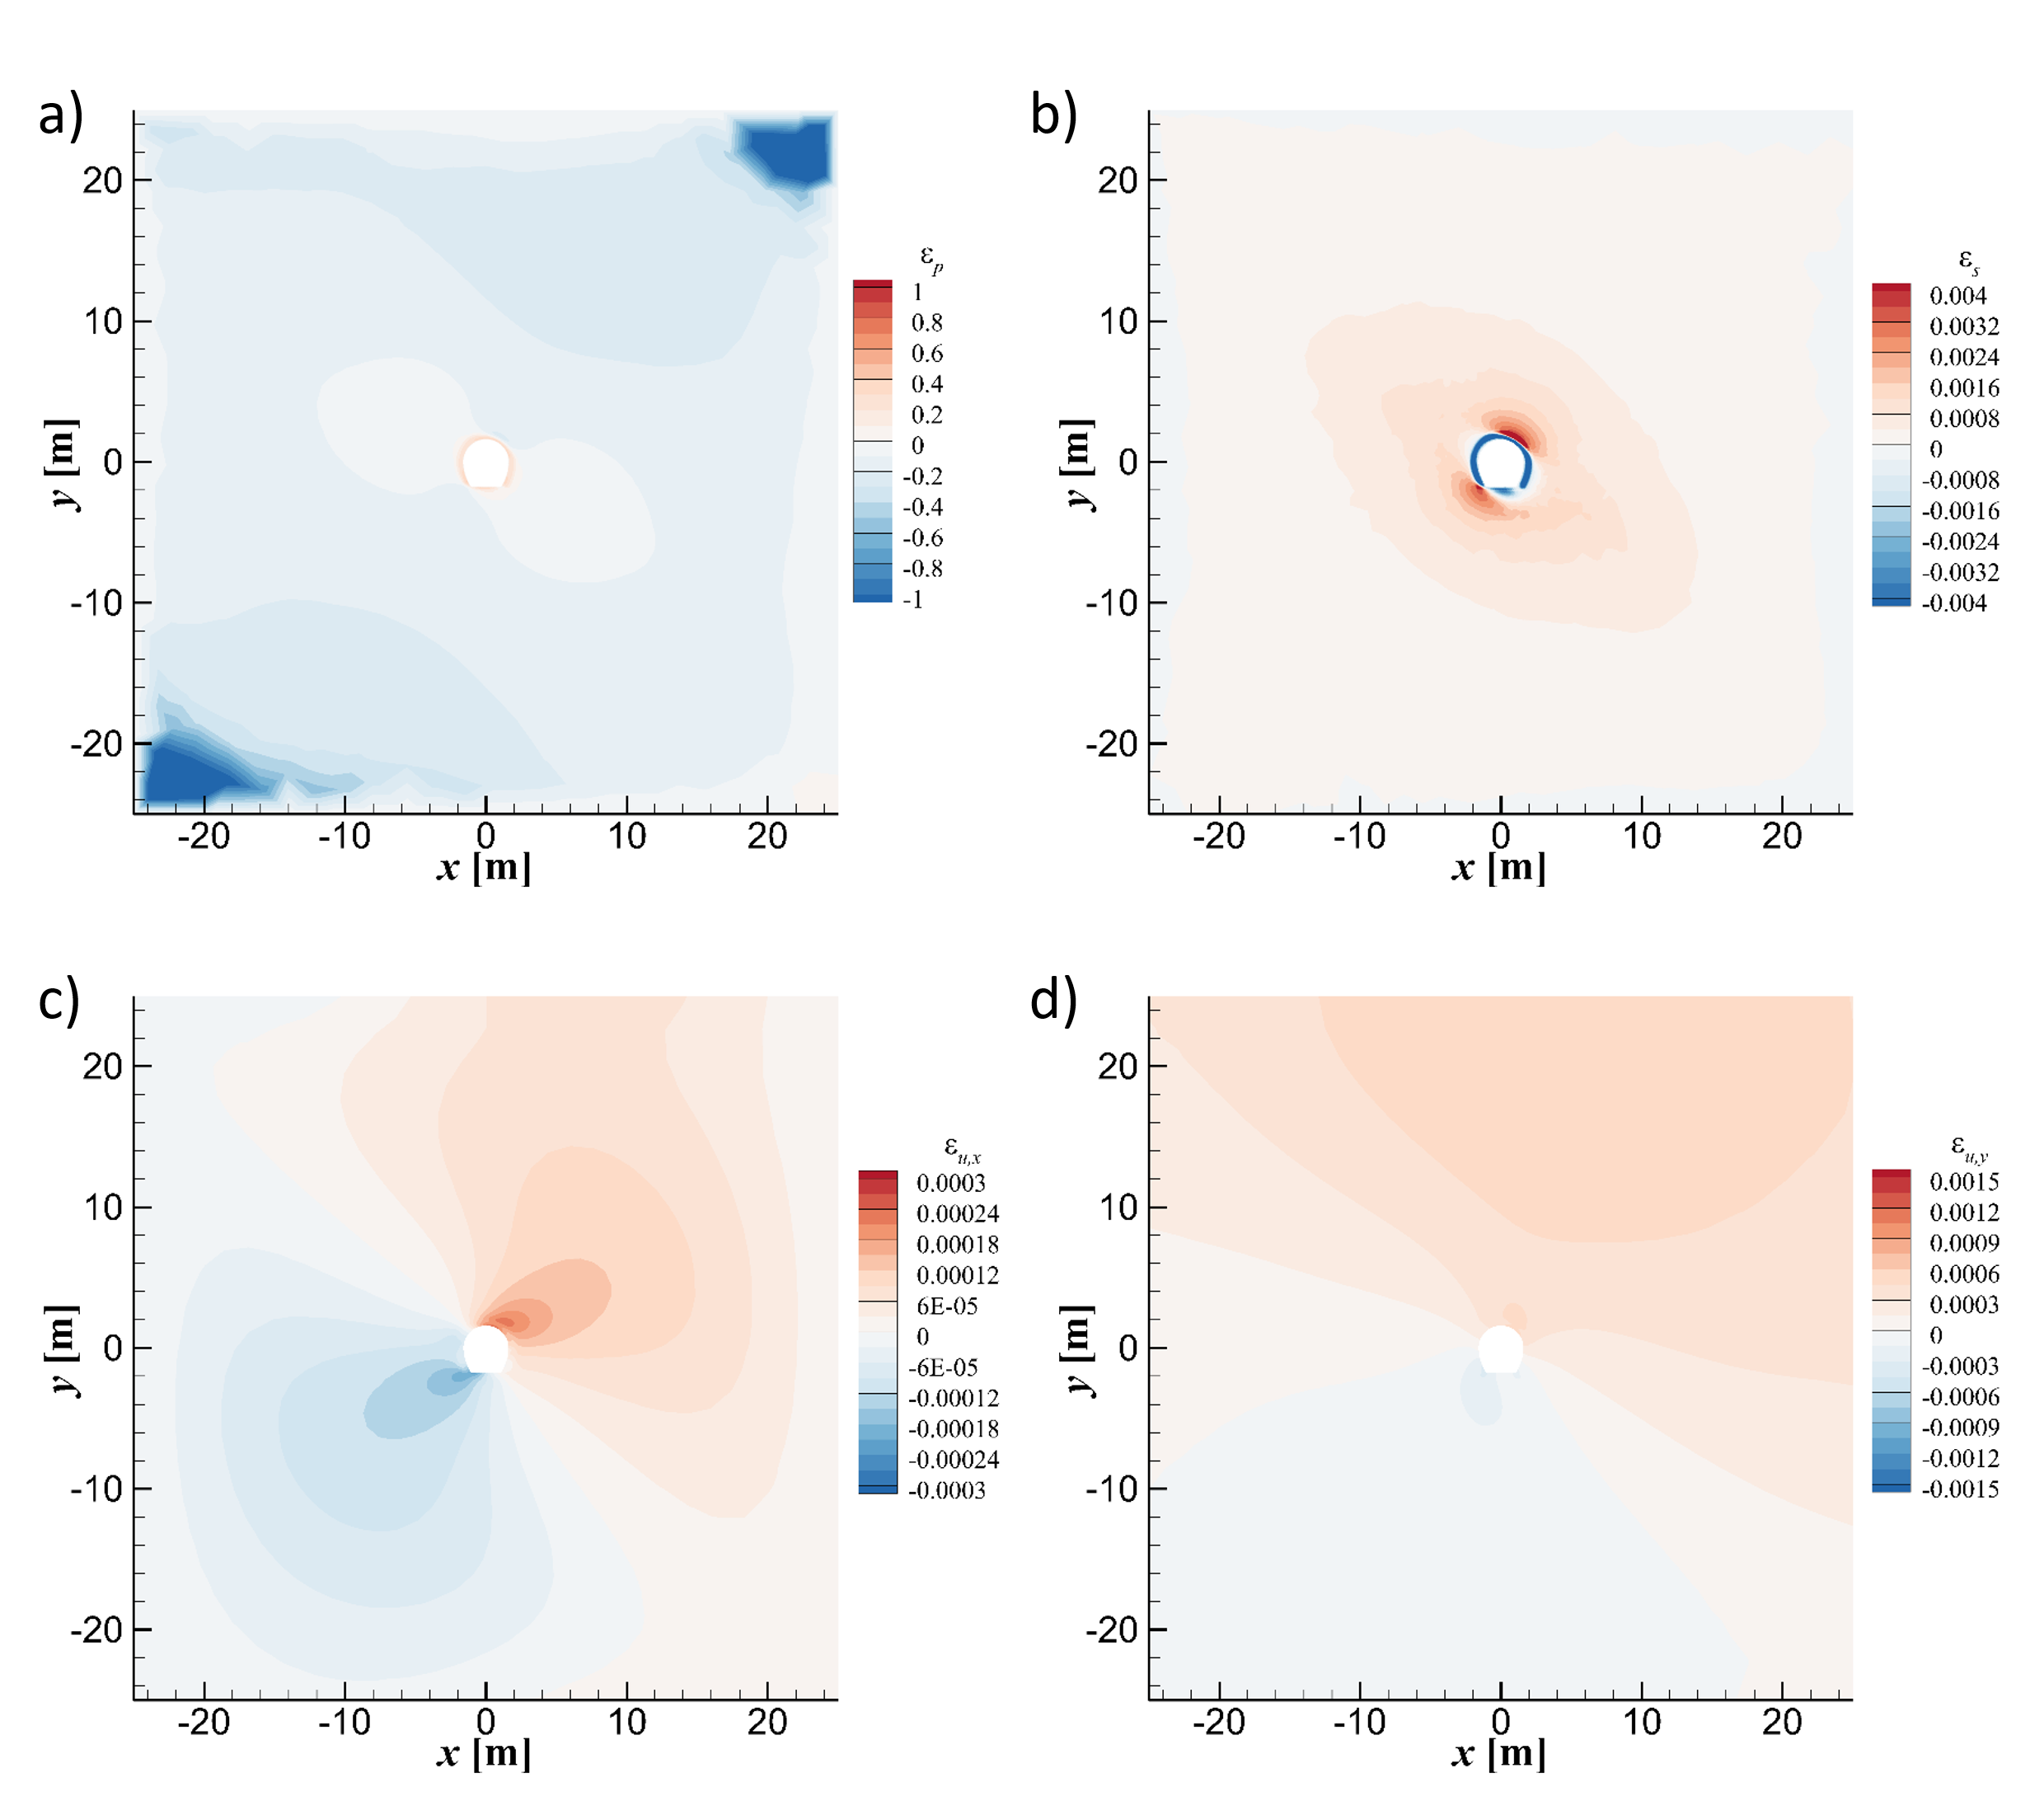
\includegraphics[width=\textwidth]{./figures/MEX10_RM_error_2d_anisotropic.png}
\caption{Deviations between OGS-5 and OGS-6 for anisotropic conditions after 20 years of simulation time.  a) Fluid pressure, b) effective saturation, c) horizontal deformation and d) vertical deformation.}
\label{fig:RM_error_2d_anisotropic}
\end{figure}

\begin{table}
 \caption{Deviations observed when comparing OGS-5 with OGS-6 for the RM process with anisotropic conditions.\label{tab:error_RM_anisotropic}}
\begin{center}
\begin{tabular}{ l | c | c | c }
 Quantity				& $\min{(\epsilon)}$ 	& $\max{(\epsilon)}$	 & RMSE  \\
 \hline
 $p_f$				 	& -1.8785 				& 0.4051 		& $1.27\cdot 10^{-1}$\\ 
 $S_\text{eff}$ 		& -0.0120 				& 0.0090		& $2.51\cdot 10^{-3}$\\		
 $u_x$					& -0.0002 				& 0.0002		& $9.48\cdot 10^{-5}$\\		 
 $u_y$ 					& -0.0004 				& 0.0006		& $2.36\cdot 10^{-4}$\\	
\end{tabular}
\end{center}
\end{table}

%%%%%%%%%%%%%%%%%%%%%%%%%%%%%%%%%%%%%%%%%%%%%%%%%%%%%%%%%%%%%%%%%%%%%%%%%%%%%%%%%%%%%%%%%
\subsection{Code performance}
%%%%%%%%%%%%%%%%%%%%%%%%%%%%%%%%%%%%%%%%%%%%%%%%%%%%%%%%%%%%%%%%%%%%%%%%%%%%%%%%%%%%%%%%%

To compare the performance of the two simulation codes, we measure the wall-clock time for the different simulations runs, which were carried out on a single core on the local \texttt{B2lx06} and \texttt{OGS02} at the BGR. Both systems are equipped with Intel Xeon E5-2690 processors. The processors on the older cluster \texttt{B2lx06} are the version 2 of this type of processor with a clock frequency of  3.0 GHz, whereas the newer cluster \texttt{OGS02} uses version 3 with a clock frequency of 2.6 GHz. Hence, we expect a similar performance for the two systems. For the analysis that follows, we only consider those simulations with a computational mesh of a total of 5463 nodes and 29,200 time steps for the entire simulation time. 

All runtimes recorded for the simulations presented in Sections \ref{sec:RF} and \ref{sec:RM} are summarized in Table \ref{tab:runtime}. The simulation carried out with OGS-5 in Section \ref{sec:RF} took 10 h and 54 min, whereas OGS-6 needed 1 h and 15 min for the same problem. Hence, the computational time of OGS-6 excels over OGS-5 by a factor of 8.6 for the "Richards Flow" model. While the simulation using "Richards Flow" was completed after 1 h 15 min, the simulation using OGS-5 with the model "Richards Mechanics" (Section \ref{sec:RM_no_M}) took 78 h and 20 min on the local cluster \texttt{B2lx06} at BGR, which is more than 3 days. This could be caused by the increased complexity of including mechanic deformation in the integration scheme (Equations \eqref{eq:linear_momentum}--\eqref{eq:hookes_law}). 

On the other hand, the computation for the setup described in Section \ref{sec:full_RM} took 81 h (isotropic conditions) and 153.5 h (anisotropic conditions) on the (faster  and newer) \texttt{OGS02} cluster, while OGS-6 needed 91.6 h (isotropic conditions) and 113.6 h (anisotropic conditions) on the (slower and older) cluster \texttt{B2lx06} to complete the task. This shows that for the computational time becomes comparable for the codes when the full "Richards Mechanics" process is considered. Nevertheless, the fact that OGS-6 uses a stronger coupling suggests that the newly developed OGS-6 is superior to its predecessor version.  A more rigorous speed test on identical hardware would be desirable to gain full insight into the enhanced capabilities of OGS-6.

\begin{table}
 \caption{Runtime for the different simulations presented in Sections \ref{sec:RF} and \ref{sec:RM}. Both systems are run by the BGR and employ Intel Xeon E5-2690 processors. Cluster \texttt{B2lx06} uses version two  with a clock frequency of 3.0 GHz, wheras cluster \texttt{OGS02} uses version 3 with a clock frequency of 2.6 GHz. \label{tab:runtime}}
\begin{center}
\begin{tabular}{ l | r | r | r  }
 Analysis		&  Software & System & Runtime [h]\\ 
 \hline
 \multirow{2}{*}{Section \ref{sec:RF}} 	& OGS-5 & \texttt{OGS02} & 10.9\\
 									& OGS-6 & \texttt{OGS02} &  1.25\\
 \hline 										
 Section \ref{sec:RM_no_M}	& OGS-6 & \texttt{B2lx06} & 78.3\\
 \hline
 \multirow{2}{*}{Section \ref{sec:full_RM} - isotropic} & OGS-5 & \texttt{OGS02} & 81\\
& OGS-6 & \texttt{B2lx06} & 91.6 \\
 \hline
 \multirow{2}{*}{Section  \ref{sec:full_RM} - anisotropic}  & OGS-5 & \texttt{OGS02} & 153.5\\
& OGS-6 & \texttt{B2lx06} & 113.6 \\
\end{tabular}
\end{center}
\end{table}

%%%%%%%%%%%%%%%%%%%%%%%%%%%%%%%%%%%%%%%%%%%%%%%%%%%%%%%%%%%%%%%%%%%%%%%%%%%%%%%%%%%%%%%%%
\subsection{Conclusions}
%%%%%%%%%%%%%%%%%%%%%%%%%%%%%%%%%%%%%%%%%%%%%%%%%%%%%%%%%%%%%%%%%%%%%%%%%%%%%%%%%%%%%%%%%

We have conducted a detailed investigation of a characteristic coupled hydro-mechanical problem of a saturating/desaturating niche in a rock laboratory to compare the accuracy of the newly developed FE-code OGS-6 to its predecessor version OGS-5. We employed characteristic properties of clayrock and apply realistic boundary conditions such as the seasonal change of air humidity  at the wall of the niche and the tranverse isotropic behavior introduced by the bedding of the clayrock in a certain angle of inclination. The aim was to reproduce the results by \cite{ziefle2018}, who successfully computed the hydro-mechanical behavior of a niche in the Mont Terri Rock Laboratory. We built the tests  with increasing complexity starting from uncoupled hydraulic effects to transverse isotropic conditions of the fully coupled hydro-mechanical process. 

As desired, we have found a high degree of agreement between the two codes for the uncoupled hydraulic process "Richards Flow". However, we found differences in the fully hydro-mechanically coupled problem "Richards Mechanics" which may be due to the different coupling schemes employed in the different codes. Further research will be needed to clarify this issue. The new code OGS-6 shows a good performance in terms of wall clock time needed to complete the simulation tasks, although more rigorous testing would be needed to get a better picture of the performance on different systems under controlled operation conditions. Furthermore, the implementation of the governing equations in OGS-6 was found to be of first order in time. The order of convergence in space was found to be 1.6. OGS-6 provides enhanced capabilities for the coupling of the two processes, such as the strongly coupled monolithic scheme that, in general, is more accurate than the weakly coupled staggered scheme. These developments provide a promising starting point for further simulations that allow for high fidelity investigations of coupled processes in clayrock.

\clearpage
\clearpage
%------------------------------------------------------------------------------
\section*{WP2: Pathways through pressure-driven percolation (clay/salt rocks)}
%------------------------------------------------------------------------------
\section{Model Exercise 2-1a (02): Fluid driven percolation in salt}
\label{sec:mex02}
%------------------------------------------------------------------------------
\Authors{Amir Sattari, Matthias Nest, Keita Yoshioka et al.}
%------------------------------------------------------------------------------
Model Exercise 2 (ME 2) investigates the fluid driven percolation (hydraulic fracking) in salt and clay stone samples under anisotropic confining stresses. The pressurized oil is injected through the pre-drilled cavity until the sudden pressure drop or increase in flow rate is observed. The main goal of this test is to determine the stress dependent fracking path and the required fracking pressure which should be higher than the minimum principle stress applied to the system. For the simulation of the fluid driven percolation, the continuum and discreet methods are considered.
%------------------------------------------------------------------------------
\subsection{Experimental set-up}
%------------------------------------------------------------------------------
The experimental tests on saltstone samples have been conducted at TU Freiberg \cite{Kamlot2009}. The cubic samples with a side length dimension of 100 §mm§ are prepared and placed in the true tri-axial apparatus \ref{fig:Amir_ME2_Saltstone_Setup}. The cubic samples are prepared with a drilled cavity length and diameter of 40 and 16 $mm$, respectively. The pressurized fluid is injected through a tubing from upper boundary and the fracking and change of flow rate is tracked. The applied two anisotropic stress configurations and the fracking paths are shown in  Figure \ref{fig:Amir_ME2_stress_state_a} and \ref{fig:Amir_ME2_stress_state_b}. The figure \ref{fig:Amir_ME2_Pressure_Time_a} and \ref{fig:Amir_ME2_Pressure_Time_b} depict the change of pressure inside of the borehole with time under the constant flow rate sequels.

\begin{figure}[!ht]
\centering
\includegraphics[width=0.5\textwidth]{figures/Amir_ME2_Saltstone_Setup.png}
\caption{ME2 setup configuration of saltstone placed inside the true tri-axial apparatus \cite{Kamlot2009}}
\label{fig:Amir_ME2_Saltstone_Setup}
\end{figure}

\begin{figure}[!ht]
\begin{subfigure}[c]{0.48\textwidth}
\includegraphics[width=1\textwidth]{figures/Amir_ME2_stress_state_1.png}
\subcaption{}
\label{fig:Amir_ME2_stress_state_a}
\end{subfigure}
\hfill
\begin{subfigure}[c]{0.48\textwidth}
\includegraphics[width=1\textwidth]{figures/Amir_ME2_stress_state_2.png}
\subcaption{}
\label{fig:Amir_ME2_stress_state_b}
\end{subfigure}
\caption{The confining (a) $1^{st}$ stress, and (b) $2^{nd}$ stress configuration setup in saltstone \cite{Kamlot2009}}
\end{figure}

\begin{figure}[!ht]
\begin{subfigure}[c]{0.48\textwidth}
\includegraphics[width=1\textwidth]{figures/Amir_ME2_Pressure_Time_1.png}
\subcaption{}
\label{fig:Amir_ME2_Pressure_Time_a}
\end{subfigure}
\hfill
\begin{subfigure}[c]{0.48\textwidth}
\includegraphics[width=1\textwidth]{figures/Amir_ME2_Pressure_Time_2.png}
\subcaption{}
\label{fig:Amir_ME2_Pressure_Time_b}
\end{subfigure}
\caption{The borehole pressure evolution under constant flow rate sequels for (a) $1^{st}$ stress, and (b) $2^{nd}$ stress configurations \cite{Kamlot2009}}
\end{figure}
%------------------------------------------------------------------------------
\subsection{Model approaches}
%------------------------------------------------------------------------------
Different numerical methods (DEM, LEM, PFM) are implemented to investigate the applicability of each model to simulate the fracking path, fracking pressure and flow rate changes in the saltstone samples. Below, the description of each model and the discussion of the results are provided. The stress dependent fracking path due to anisotropic stress configurations are captured by both continuum and discrete models. 
%------------------------------------------------------------------------------
\subsubsection*{Discrete-Element-Model (DEM)}
Figure \ref{fig:ME2_DEM_model_setup} shows the elements and interfaces/grain boundaries used for DEM simulation of the modeling exercise 2. For both of the stress states, the identical elements and interfaces were used. Simulation results from the first stress configuration are shown in \ref{fig:ME2_DEM_stress1_result}.

\begin{figure}[!ht]
\centering
\includegraphics[width=0.45\textwidth]{figures/ME2_DEM_model.pdf}
\includegraphics[width=0.45\textwidth]{figures/ME2_DEM_grain.pdf}
\caption{ME2 DEM model set-up.}
\label{fig:ME2_DEM_model_setup}
\end{figure}

\begin{figure}[!ht]
\centering
\includegraphics[width=0.45\textwidth]{figures/ME2_DEM_stress1_vertical.pdf}
\includegraphics[width=0.45\textwidth]{figures/ME2_DEM_stress2_side.pdf}
\caption{ME2 DEM model results for the stress configuration 2.}
\label{fig:ME2_DEM_stress1_result}
\end{figure}

\begin{figure}[!ht]
\centering
\includegraphics[width=0.45\textwidth]{figures/ME2_DEM_stress2_vertical.pdf}
\includegraphics[width=0.45\textwidth]{figures/ME2_DEM_stress2_side.pdf}
\caption{ME2 DEM model results for the stress configuration 2.}
\label{fig:ME2_DEM_stress2_result}
\end{figure}

\subsubsection*{Lattice-Element-Model (LEM)}

The dual lattice model, described in the section \ref{Section:HMLattice}, is implemented to simulate the fluid driven percolation in the saltstone samples. The applied hydraulic pressures are transformed into the mechanical model using the weak coupling scheme and subsequently the elements failure and change of hydraulic aperture are determined and transformed back to the hydro model. The considered mass conservation law results in the prediction of flow rate and change of reservoirs pressure as well as the flow and fracking paths, which are then compared to the experimental data. The total number of mechanical and conduct lattice elements are approximately 10000 and 80000, respectively (\ref{fig:Amir_ME2_LEM_a_model}).  The experimental setup shown in \ref{fig:Amir_ME2_stress_state_a} is simulated using  the dual LEM and the developed fractures and flow path are shown in \ref{fig:Amir_ME2_LEM_a_model_Fracture} and \ref{fig:Amir_ME2_LEM_a_model_Flow}. Similarly, the fracture surfaces and flow paths under the second stress configuration \ref{fig:Amir_ME2_stress_state_b} are illustrated in \ref{fig:Amir_ME2_LEM_b_model_Fracture} and \ref{fig:Amir_ME2_LEM_b_model_Flow}, respectively. In these simulations the Young's modulus is assumed to be 30 $GPa$. In Figure \ref{fig:Amir_ME2_LEM_a_model_Fracture}, the fracking path propagation in the horizontal direction (on the top surface) similar to the experimental result (Figure \ref{fig:Amir_ME2_stress_state_a}) is observed. 

\begin{figure}[!ht]
\centering
\includegraphics[width=0.5\textwidth]{figures/Amir_ME2_LEM_a_model.png}
\caption{The boundary condition in the lattice model, cross-section view}
\label{fig:Amir_ME2_LEM_a_model}
\end{figure}

\begin{figure}[!ht]
\begin{subfigure}[c]{0.48\textwidth}
\includegraphics[width=1\textwidth]{figures/Amir_ME2_LEM_a_model_Fracture.png}
\subcaption{}
\label{fig:Amir_ME2_LEM_a_model_Fracture}
\end{subfigure}
\hfill
\begin{subfigure}[c]{0.48\textwidth}
\includegraphics[width=1\textwidth]{figures/Amir_ME2_LEM_a_model_Flow.png}
\subcaption{}
\label{fig:Amir_ME2_LEM_a_model_Flow}
\end{subfigure}
\caption{ The simulation of fluid driven percolation shown in \ref{fig:Amir_ME2_stress_state_a}: The cross-section of the (a) fracking surfaces (red), and (b) flow path surfaces (blue)}
\end{figure}

\begin{figure}[!ht]
\begin{subfigure}[c]{0.48\textwidth}
\includegraphics[width=1\textwidth]{figures/Amir_ME2_LEM_b_model_Fracture.png}
\subcaption{}
\label{fig:Amir_ME2_LEM_b_model_Fracture}
\end{subfigure}
\hfill
\begin{subfigure}[c]{0.48\textwidth}
\includegraphics[width=1\textwidth]{figures/Amir_ME2_LEM_b_model_Flow.png}
\subcaption{}
\label{fig:Amir_ME2_LEM_b_model_Flow}
\end{subfigure}
\caption{ The simulation of fluid driven percolation shown in \ref{fig:Amir_ME2_stress_state_b}: The cross-section of the (a) fracking surfaces (red), and (b) flow path surfaces (blue)}
\end{figure}
%------------------------------------------------------------------------------
\subsubsection*{Finite-Element-Model: Variational-Phase-Field (VPF)}
%------------------------------------------------------------------------------
\todo[inline]{[UFZ](KY): Please add results}
%------------------------------------------------------------------------------
\subsection{Results and discussion}

 The stress dependent fracking path in saltstone samples due to the defined anisotropic stress configurations is investigated. To do so,  The experimental test data are taken from the literature and the validation of the numerical models is performed. The VPF results .... 
 \todo[inline]{Amir: Keita Please add discussion}. 
 
 The implemented lattice model depicts the fracking paths in Figure  \ref{fig:Amir_ME2_LEM_a_model_Fracture} and \ref{fig:Amir_ME2_LEM_b_model_Fracture}. For a $1^{st}$ and $2^{nd}$ stress configurations the fracking pressure is found to be 13.2 and 7.1 $MPa$, respectively. Both values are slightly higher than the given fracking pressure from the literature. However, the fracking pressures in both cases are higher than the minimum principle stresses. The fracking paths shown with red surfaces match the experimental results, where the $1^{st}$ stress configurations results in horizontal fracking paths and the $2^{nd}$ stress configurations results in vertical fracking paths. The discrete element method is also able to simulate the fracking path similar to the experimental results. The application of the numerical methods for quantitative comparison of the simulation results with the experimental data needs further investigation. 

%------------------------------------------------------------------------------
\todo[inline]{[CAU]: Please add discussion}
%------------------------------------------------------------------------------


\clearpage
%------------------------------------------------------------------------------
\section[MEX 2-1b: Fluid driven percolation in clay]{Model-Experiment-Exercise MEX 2-1b:\\Fluid driven percolation in clay}
\label{sec:mex2-1b}
%------------------------------------------------------------------------------
\Authors{Amir Shoarian Sattari, Keita Yoshioka}
%------------------------------------------------------------------------------
In this model exercise, the fracking path and fracking pressure for a sandy Opalinus claystone sample under two different initial stress configurations are investigated. In addition to the stress configurations and due to the high anisotropy of the claystone samples, it is expected that due to the weak bond between the embedded layers, the fracking path and flow will be governed by orientation of the embedded layers. 
\index{fracturing processes}
%------------------------------------------------------------------------------
\subsection{Experimental set-up}
%------------------------------------------------------------------------------
The cubic Opalinus claystone samples are prepared in the side dimension of 43 $mm$ and with the drilled cavity length and diameter of 20 and 8 $mm$ (Figure \ref{fig:Amir_Percolation_Adapter}). The applied mechanical stress configurations are as shown in Fig. \ref{fig:Amir_Percolation_Stress_1} and \ref{fig:Amir_Percolation_Stress_2}. The samples embedded layering orientations are shown in Fig. \ref{fig:Amir_Percolation_Orientation1} and \ref{fig:Amir_Percolation_Orientation2}, where in the first case the applied oil pressure is perpendicular to the layering orientations and in the second case it is parallel to the layering orientations.

\begin{figure}[!ht]
\begin{subfigure}[c]{0.48\textwidth}
\centering
\includegraphics[width=5cm,height=4cm]{figures/Amir_Percolation_Stress_1.png}
\subcaption{}
\label{fig:Amir_Percolation_Stress_1}
\end{subfigure}
\hfill
\begin{subfigure}[c]{0.48\textwidth}
\centering
\includegraphics[width=5cm,height=4cm]{figures/Amir_Percolation_Stress_2.png}
\subcaption{}
\label{fig:Amir_Percolation_Stress_2}
\end{subfigure}
\caption{The applied (a) $1^{st}$, and (b) the $2^{nd}$ stress configurations}
\end{figure}

\begin{figure}[!ht]
\begin{subfigure}[c]{0.48\textwidth}
\centering
\includegraphics[width=4cm,height=4cm]{figures/Amir_Percolation_Orientation1.png}
\subcaption{}
\label{fig:Amir_Percolation_Orientation1}
\end{subfigure}
\hfill
\begin{subfigure}[c]{0.48\textwidth}
\centering
\includegraphics[width=4cm,height=4cm]{figures/Amir_Percolation_Orientation2.png}
\subcaption{}
\label{fig:Amir_Percolation_Orientation2}
\end{subfigure}
\caption{The orientation of the embedded layers (a) perpendicular, and (b) parallel to the direction of the borehole pressure configuration}
\end{figure}

The syringe pump is used to pump the pressurized hydraulic oil (up to 517 $Bar$) into the sample and with gradually increasing the pressure the fracking process is carried out. In the first setup, the hydraulic fracking is initiated at 23 $MPa$ and the clear flow paths through the embedded layering surfaces is observed \ref{fig:Amir_Percolation_Frack_a}. Similarly, for the second test setup, the hydraulic fracking is initiated at 10 $MPa$ through the embedded layering surfaces as shown in Fig. \ref{fig:Amir_Percolation_Frack_b}. Fig. \ref{fig:Amir_Percolation_Flow_a} and \ref{fig:Amir_Percolation_Flow_b} illustrates the borehole pressure evolution with flow volume change obtained from the experimental data. The initial volume of the pump is around 265 $mL$,

\begin{figure}[!ht]
\begin{subfigure}[c]{0.48\textwidth}
\centering
\includegraphics[width=5cm,height=5cm]{figures/Amir_Percolation_Frack_a.png}
\subcaption{}
\label{fig:Amir_Percolation_Frack_a}
\end{subfigure}
\hfill
\begin{subfigure}[c]{0.48\textwidth}
\centering
\includegraphics[width=5cm,height=5cm]{figures/Amir_Percolation_Frack_b.png}
\subcaption{}
\label{fig:Amir_Percolation_Frack_b}
\end{subfigure}
\caption{The fracking paths through the Opalinus claystone (a) $1^{st}$ stress configuration, and (b) $2^{nd}$ stress configuration}
\end{figure}

\begin{figure}[!ht]
\begin{subfigure}[c]{0.48\textwidth}
\includegraphics[width=1\textwidth]{figures/Amir_Percolation_Flow_a.png}
\subcaption{}
\label{fig:Amir_Percolation_Flow_a}
\end{subfigure}
\hfill
\begin{subfigure}[c]{0.48\textwidth}
\includegraphics[width=1\textwidth]{figures/Amir_Percolation_Flow_b.png}
\subcaption{}
\label{fig:Amir_Percolation_Flow_b}
\end{subfigure}
\caption{The borehole pressure vs. flow volume for a Opalinus claystone (a) $1^{st}$ stress configuration, and (b) $2^{nd}$ stress configuration}
\end{figure}

%------------------------------------------------------------------------------
\subsection{Model approaches}
%------------------------------------------------------------------------------
\subsubsection*{Lattice-Element-Model (LEM)}

With the implemented lattice model, the effect of the Opalinus claystone anisotropy on the fracking paths and fracking pressure is investigated. The similar approach as described in section \ref {sec:mex01} is taken to define the layering orientations in the medium. It is assumed that the interface elements bonding two different layers have 5 times weaker strength than the same layers bond (found in \ref{sec:Brazilian_Disk_Exp}). The generated 3D setup using the LEM is shown in Fig. \ref{fig:Amir_Percolation_Setup_a} and \ref{fig:Amir_Percolation_Setup_b}. The total number of mechanical and conduct lattice elements are approximately 28000 and 200000, respectively.
The percolation tests under the two stress configurations and with different embedded layering orientations are simulated. Fig. \ref{fig:Amir_ME2_B_Fracture_a} and \ref{fig:Amir_ME2_B_Fracture_b} depict the fracking surfaces (red) for the $1^{st}$ and $2^{nd}$ stress configurations, respectively. It is observed, similar to the experimental result, that the layering orientation controls the flow paths in Opalinus claystone samples. 

\begin{figure}[!ht]
\begin{subfigure}[c]{0.48\textwidth}
\centering
\includegraphics[width=5cm,height=5cm]{figures/Amir_Percolation_Setup_a.png}
\subcaption{}
\label{fig:Amir_Percolation_Setup_a}
\end{subfigure}
\hfill
\begin{subfigure}[c]{0.48\textwidth}
\centering
\includegraphics[width=5cm,height=5cm]{figures/Amir_Percolation_Setup_b.png}
\subcaption{}
\label{fig:Amir_Percolation_Setup_b}
\end{subfigure}
\caption{The generated 3D domain in lattice model for the (a) $1^{st}$ stress configuration, and (b) $2^{nd}$ stress configuration}
\end{figure}

\begin{figure}[!ht]
\begin{subfigure}[c]{0.48\textwidth}
\centering
\includegraphics[width=5cm,height=5cm]{figures/Amir_ME2_B_Fracture_a.png}
\subcaption{}
\label{fig:Amir_ME2_B_Fracture_a}
\end{subfigure}
\hfill
\begin{subfigure}[c]{0.48\textwidth}
\centering
\includegraphics[width=5cm,height=5cm]{figures/Amir_ME2_B_Fracture_b.png}
\subcaption{}
\label{fig:Amir_ME2_B_Fracture_b}
\end{subfigure}
\caption{The fracking surfaces (red) for the (a) $1^{st}$ , and (b) $2^{nd}$ stress configurations}
\end{figure}

\begin{figure}[!ht]
\begin{subfigure}[c]{0.48\textwidth}
\centering
\includegraphics[width=5cm,height=5cm]{figures/ME2b_init_para.png}
\subcaption{}
\end{subfigure}
\hfill
\begin{subfigure}[c]{0.48\textwidth}
\centering
\includegraphics[width=5cm,height=5cm]{figures/ME2b_init_orth.png}
\subcaption{}
\end{subfigure}
\caption{3D computation domain of VPF for (a) $1^{st}$ stress configuration, and (b) $2^{nd}$ stress configuration.}
\label{fig:VPF_ME2_B_init}
\end{figure}

\subsubsection*{Finite-Element-Model: Variational Phase-Field (VPF)}
Using the variational phase-field model presented in this study, impacts of the anisotropy induced by the lamination parallel and orthogonal of the Opalinus claystone will be studied through 3D computational domains (Figs~\ref{fig:VPF_ME2_B_init}).

%------------------------------------------------------------------------------
\subsection{Results and discussion}

The experimental results form the fluid driven percolation tests on Opalinus claystone show the effect of the anisotropy on fracking paths and stress distribution. The fracking and leakage through the weak bond along the embedded layers is observed. However, more experimental data under different principle stress configurations are required to detect and analyse the stress distribution and the frack paths dependency on the anisotropy. For both samples tested here the fracking stress was higher than the applied minimum principle stress. For a $1^{st}$ stress configuration, the fracking pressure was much higher than applied maximum principle stress, which can be due to an error in the experimental results. The lack of the pre-defined notch during the sample preparation also can lead to higher fracking stresses. The fracking in $2^{nd}$ stress configuration was subtle and no pressure drop is recorded. The increase in the flow volume at the borehole pressure of 10 $MPa$ indicate the initiation of the fracking process. The dual lattice model is implemented to simulate the hydraulic fracking in Opalinus claystone. The anisotropy is implemented in the model, where the bond strength between the embedded layers is assumed to be 5 times weaker than a same layer bond. Due to this assumption which is found from Brazilian disk results (see section \ref{sec:Brazilian_Disk_Exp}), the fracking along the embedded layers is observed. The fracking pressures found to be higher than minimum principle stresses. However, more research for quantitative comparison of the results is needed. 
%------------------------------------------------------------------------------

\clearpage
%------------------------------------------------------------------------------
%\section{Model Exercise 2-2 (03): Pressure driven percolation (healing)}
\label{sec:mex03}
%------------------------------------------------------------------------------
\Authors{Mathias Nest, Keita Yoshioka et al.}
%------------------------------------------------------------------------------
\subsection{Experimental set-up}
%------------------------------------------------------------------------------
One of the most important properties of barriers formed by salt or clay is their ability to close cracks and heal through creep. This means, that the materials can regenerate and regain their impermeability, after damage due to, e.g. excavation activities or  pressure driven percolation because of a temporary violation of the minimal stress criterion.

\begin{figure}[!ht]
\centering
\includegraphics[width=8cm]{figures/mex3-exper-setup.png}
\caption{Rock salt sample, borehole geometry, detail of metal pipe.}
\label{fig:ME3-exper-setup}
\end{figure}

In this study we focus on the sealing of pathways and healing of cracks in salt and clay by measuring and simulating their gas permeability after damage has been done. 

For rock salt, we prepared cylindrical samples with a height of 20 cm and a diameter of 10 cm, with a borehole to the center, so that a gas pressure could be applied to a small area at the center. Initially all samples were placed under isostatic stress of 50 MPa for one day, to consolidate them. For the actual experiments the isostatic stresses were then changed to 10 MPa, 30 MPa, and 50 MPa, respectively. Before the gas pressure was applied, the plates which applied the axial stress were lock in place (''displacement boundary condition''). The gas pressure was increased in small steps, until a gas flow was detected. In all three cases a gas flow was detected before the percolation threshold was reached, which indicates that the samples suffered micro-fractures during preparation. After the last increase of the pressure, the flow rate was monitored for 24 to 70 hours under constant conditions.

\begin{figure}[!ht]
\centering
\includegraphics[width=1\textwidth]{figures/mex3-stresses-flows-v2.png}
\caption{Axial and confining stresses, gas pressures, and observed flow rates.}
\label{fig:ME3-stresses-flows}
\end{figure}
 
\begin{figure}[!ht]
\centering
\includegraphics[width=9cm]{figures/mex3-perme-time-comparison.png}
\caption{Reduction of the permeability under different hydrostatic stress conditions.}
\label{fig:ME3-perme-exp}
\end{figure}

The flow rate can be converted into permeabilities, which are shown in Fig. \ref{fig:ME3-perme-exp}. For all three cases a reduction of the permeability is found,  showing that the cracks are narrowing and slowly closing. The abrupt and discontinuous manner of the change of the flow rate makes it difficult to identify time-scales of the processes involved. In the case of 10 MPa confining stress one can distinguish two phases. Between 3 and 24 hours after the start of the experiment, one can fit (admittedly only very crude) a time-scale of about 4.5 hours. Some larger pathways seem to close abruptly. After that, the pathways narrow only very slowly, presumably by creep processes, on a time-scale of about 1000 hours. In the cases of 30 MPa and 50 MPa we find time-scales of 30 hours and 11 hours, respectively. At least here, faster creep under higher stress is found as expected for the general trend.

\begin{figure}[!ht]
\centering
\includegraphics[width=9cm]{figures/mex3-claysample.png}
\caption{Left: Setup of the fracture closing experiment with Opalinus clay. Right: One of the samples.}
\label{fig:ME3-clay-setup}
\end{figure}

The Opalinus clay samples were prepared slightly differently, see Fig. \ref{fig:ME3-clay-setup}. The cylinders had a height of 160 mm and a diameter of 80 mm. Two boreholes were used, to avoid that under isostatic stress conditions the gas flows in a radial direction. Again it turned out, that the sample preparation had induced dilatant damage, so that a significant gas flow was already detected before the gas pressure reached the value of the mechanical stress. The subsequent results were obtained at a pressure of 0.5 bar. 

\begin{figure}[!ht]
\centering
\includegraphics[width=9cm]{figures/mex3-senkrecht-alle.png}
\caption{Evolution of gas flow rates under different isostatic stresses.}
\label{fig:ME3-clay-flows}
\end{figure}

The results are shown in Fig. \ref{fig:ME3-clay-flows}. Initially, a stress of 7 MPa was applied, and the gas flow decreased from 38 ml/min to 24 ml/min in the course of about 100 hours. Then the stress was reduced to 5 MPa, which lead to an increased flow of 26 ml/min. Again, a decreasing rate was observed, reaching 6 ml/min after 400 hours. Finally the stress was increased to 9 MPa, and the rate dropped from 4.4 to 1.8 ml/min. So in all three cases the microfractures from the sample preperation were closing slowly, as a first step towards healing. The difference to the previous experiment with rock salt is stark. The clay reacted much more smoothly, and good fits to exponential decays could be obtained. The reason is the much smaller grain size in the clay, which permits much smaller displacements. In addition, the general trend, that the time scales decrease as the stresses are increased, is observed as expected. 

%------------------------------------------------------------------------------
\subsection{Model approaches}
%------------------------------------------------------------------------------
\subsubsection*{Discrete-Element-Model (DEM)}

The closure of cracks and the healing of rock salt after plastic deformation has been rarely looked upon and studied in detail. The purpose of this exercise is therefore to develop a phenomenological model, which can be incorporated into the 3DEC software. The mechanistic idea behind the process is shown in Fig. \ref{fig:ME3-crack-stre} Cracks have a rough surface, with high deviatoric stresses where they are in contact. This concentration of stress can lead to the abrupt abrasions observed above, and also to an increased creep rate. 

\begin{figure}[!ht]
\centering
\includegraphics[width=8cm]{figures/mex3-crack-stresses.png}
\caption{Locations of high deviatoric stress in a crack. The deviatoric stress drives creep, which leads to a closing of the crack.}
\label{fig:ME3-crack-stre}
\end{figure}

In 3DEC the fluid flow is modelled using fluid knots, where apertures between two grains are defined. The size of the aperture depends on an elastic spring constant, the pressure, and two cut-off values, see Fig. \ref{fig:ME3-dem-apert}. There, $a_{max}$ and $a_{res}$ are the maximally and minimally allowed fluid apertures, and $a_0$ is the aperture when the normal stress $\sigma_N$ is equal to the fluid pressure $p$. In the following simulation we used $a_{res}$ = $a_0$ = 10$^{-7}$ m. The narrowing of the crack is then modelled by decreasing $a_{max}$ with time. 

\begin{figure}[!ht]
\centering
\includegraphics[width=8cm]{figures/mex3-aperture.png}
\caption{Schematic representation of the relation between aperture on grain boundaries and effective stress in 3DEC.}
\label{fig:ME3-dem-apert}
\end{figure}

The net effect of this approach is hard to predict, because the total fluid flow through the sample depends on a complex network of fluid knots with different orientations and normal stresses. Two approaches were tried: 

\begin{equation}
a_{max,n+1} = c \cdot a_{max,n} \quad \mbox{ with } 0<c<1
\end{equation}
and
\begin{equation}
a_{max,n+1} = a_{max,n} - \Delta a \quad .
\end{equation}

\begin{figure}[!ht]
\centering
\includegraphics[width=8cm]{figures/mex3-flowrate-run3beide.png}
\caption{Pressure driven percolation and subsequent crack closure.}
\label{fig:ME3-flowrate-beide}
\end{figure}


The model setup used for this simulation was the same as in section \ref{sec:mex02}. The first two phases of the simulation agree with the simulation of the pressure driven percolation. A fluid pressure was applied to the internal cavity, and after a while liquid started to leak out (see phase I in Fig. \ref{fig:ME3-flowrate-beide}). After about 2.5 s the leak rate converged to a near constant level (phase II). From this point on, the simulation was run (phase III) in two different versions, corresponding to the two different equations above for the decrease of $a_{max}$. 

For the linear decrease of the maximum aperture we find a decrease of the flow rate that is not exponential as in the experiment (nor is it linear). For the exponential decrease we used $c$ = 0.9659 and applied this value every 100000th fluid timestep. (The full simulation required more than 10 million timesteps.) In this case a very good exponential fit with a time scale of 0.63 s could be obtained. It should be noted that in this simple setup, two time scales are actually mixed, which in reality are separated: In reality, creep (and thus the narrowing of the cracks) works much slower than the fluid dynamics. But as this exercise is a proof of concept, and serves to obtain a basic understanding of how how to model the phenomenon of crack closure, we accepted this approximation. 

\subsubsection*{Finite-Element-Model: Variational Phase-Field (VPF)}

\begin{figure}[!ht]
\begin{subfigure}[c]{0.49\textwidth}
\includegraphics[width=1\textwidth]{figures/ME3_pres.png}
\subcaption{ME3 VPF model set up for the model exercise 3}
\label{fig:ME3_VPF_model}
\end{subfigure}
\hfill
\begin{subfigure}[c]{0.49\textwidth}
\includegraphics[width=1\textwidth]{figures/ME3_CrackWidth.png}
\subcaption{ME3 VPF crack width}
\label{fig:ME3_VPF_crack width}
\end{subfigure}
\caption{ME3 VPF preliminary}
\label{fig:VPF_ME2_creep}
\end{figure}

Implementation of the crack healing through creep model within the OGS variational phase-field model is being planned.
Crack opening (fracture width) is not a directly computed variable within the variational phase-field model, instead it is computed currently by taking a line integral~\cite{Yoshioka2020} as:
\begin{equation}
\left \llbracket \vec{u}\cdot \vec{n}_\Gamma \right\rrbracket
\approx \int_{l} \vec{u} \cdot \nabla v .
\label{eq:width_line_integral}
\end{equation}
where $l$ is the line that follows the normal direction to the crack $\Gamma$.
With a creep model, the displacement will be decomposed into the elastic $\vec{u}^e$ and the creep part $\vec{u}^c$ as $\vec{u} = \vec{u}^e+\vec{u}^c$, and the crack opening can be computed then by
\begin{equation}
\left \llbracket \vec{u}\cdot \vec{n}_\Gamma \right\rrbracket
\approx \int_{l} \vec{u}^e \cdot \nabla v .
\label{eq:width_line_integral}
\end{equation}
As $\vec{u}^c$ evolves with time, the crack opening will be subject to change and be able to simulate the aperture change observed in the experiments.
A preliminary attempt to calculate the fracture aperture from the elastic response only is shown in  Fig~\ref{fig:VPF_ME2_creep}.

%------------------------------------------------------------------------------
\subsection{Results and discussion}
%------------------------------------------------------------------------------
\todo[inline]{[UFZ] Please add results and discussion}
\todo[inline]{[UFZ] MEX 2-2 requires salt mechanics coupling and has not been done yet. It will follow once the MEX 2-b, 2-3, 3-3 are finished.}
\clearpage
%------------------------------------------------------------------------------
%\section[MEX 2-3: Pressure driven percolation]{Model-Experiment-Exercise 2-3:\\Effect of compressibility on pressure driven percolation}
\label{sec:mex04}
%------------------------------------------------------------------------------
\Authors{Mathias Nest, Amir Shoarian Sattari, Keita Yoshioka}
%------------------------------------------------------------------------------
\subsection{Model set-up}
%------------------------------------------------------------------------------
Salt barriers do not only protect mines against the intrusion of ground water, but they can also be important to keep substances securely isolated in underground repositories and reservoirs. Examples include caverns for gas and oil, as well as repositories for toxic or radioactive waste. In this model exercise we look at the difference between the pressure driven percolation of liquids and gases, which is not only due to their different viscosities, but also to their different response to a change in the available volume. 

Liquids like brine react with a large change in pressure, because of their rather high bulk modulus $K$:
\begin{equation}
dp = -K \frac{dV}{V}
\end{equation}
Gases, which can be described approximately with the ideal gas equation
\begin{equation}
pV=nRT
\end{equation}
\index{ideal gas law}
show a far smaller change in pressure. In this model exercise we explore this difference in a setup similar to the one in \MEXtwo~, under the assumption, that there is only a finite amount of substance available to spread into the rock salt. Another way to put this is, that a lab-scale model of the in-situ experiment \MEXeleven~ is set up. 

The basic reasoning behind the exercise is as follows: The total mass of the brine or gas is conserved, and consists of the mass in the reservoir $M_R$, the mass on the interfaces of the grains $M_I$, and the mass $M_L$ that has leaked out of the sample.
\begin{equation}
M = M_R + M_I + M_L \quad \mbox{= conserved}
\end{equation}
$M_I$ is part of the model, $M_L$ can be calculated using absorbing boundaries at the surface of the sample, and from the knowledge of the total amount $M$ that is present initially, the mass that remains in the reservoir $M_R$ can be calculated. This way, it is not necessary to model the reservoir (gas cylinder or brine container) explicitly. From the changing $M_R$ under the assumption of a fixed reservoir volume the change of the pressure in the reservoir, which drives the pressure driven percolation, can be calculated. Initially, at time $t=0$, $M_I=M_L=0$, and the pressure in the reservoir is high enough to open pathways between grains. Then, pressures and the extent of the distribution of the substances is monitored. 

\begin{figure}[!ht]
\centering
\includegraphics[width=1\textwidth]{figures/mex4-dem-setup.png}
\caption{a) Stress boundary condition b) discrete grain structure of 3DEC model c) grain boundaries/interfaces d) initial pressure on grain boundaries}
\label{fig:ME4-dem-setup}
\end{figure}

%------------------------------------------------------------------------------
\subsection{Model approaches}
%------------------------------------------------------------------------------
\subsubsection*{Discrete-Element-Method (DEM)}

For the numerical model in 3DEC the same setup was used as in MEX 2, see Fig. \ref{fig:ME4-dem-setup}. An initial reservoir pressure $p_R$ of 12 MPa, between principal stress $\sigma_2$ and $\sigma_3$, was chosen, to allow percolation. The bulk modulus of the brine was set to 2 GPa. Various reservoir volumes were tested, and  $V_R$ = 13 litres was found to give the clearest difference between gas and liquid.
For the simulation the masses $M_I$ and $M_L$ were calculated every 25 time steps. From this, the mass in the reservoir was calculated, and converted into a pressure by the constitutive relations above. The new reservoir pressure was then applied as an updated boundary condition as shown in Fig. \ref{fig:ME4-dem-setup} d). 

\begin{figure}[!ht]
\centering
\includegraphics[width=1\textwidth]{figures/me4-3dec-comparison.png}
\caption{Pressure evolution in a finite size gas/liquid reservoir.}
\label{fig:ME4-3dec-comp}
\end{figure}

\begin{figure}[!ht]
\centering
\includegraphics[width=1\textwidth]{figures/me4-3dec-vertcuts.png}
\caption{Final pressure distributions. The brine (left) gets stuck, the gas (right) reaches the boundaries and leaks out.}
\label{fig:ME4-3dec-vertcuts}
\end{figure}

Figure \ref{fig:ME4-3dec-comp} shows that there is a stark difference. The high bulk modulus of the brine leads to a very fast drop in pressure, while the gas pressure stays almost constant for quite a while. It should be mentioned that the time steps do not correspond to a physical timescale, because the rate of the fluid flow between adjacent fluid knots in the model was artificially increased, and not derived from the aperture between two grains. Still, the qualitative difference persists. The brine pressure drops so fast, that the liquid becomes stuck inside the cube (Fig. \ref{fig:ME4-3dec-vertcuts} left), while the gas pressure decreases only after a significant amount leaked from the sample (Fig. \ref{fig:ME4-3dec-vertcuts} right). In addition, it should be noted that the brine pressure does not fall below 9.3 MPa, although the minimal principal stress is only 8 MPa. This is because of two effects: First, in order for pressure driven percolation to take place, the fluid pressure has to overcome the normal stress on the grain boundaries, which is a composition of all three external stresses due to the tilted orientations. Second, the fluid has to overcome the tensile strength, set to 1 MPa, of the joints, too. 

\subsubsection*{Lattice-Element-Method (LEM)}

In order to simulate the compressibility effect with the lattice model, the similar setup as shown in Fig. \ref{fig:ME4-dem-setup} is considered. The initial reservoir pressure is set to be 12 $MPa$, which is higher than minimum principal stress of 8 $MPa$. The bulk modulus of brine is assumed to be 2 $GPa$ and the volume of reservoir to be 13 $L$. The total number of mechanical and conduct lattice elements are approximately 10000 and 80000, respectively. The rate of pressure drop in the reservoirs storing the brine and gas (methane) is investigated. The hydro model explained in section \ref{Section:HMLattice} is implemented to grant the mass conservation in the domain. The boundary reservoir pressure is not constant and with the fluid/gas transport in the medium it gradually drops. Due to the high bulk modulus of brine it is expected that the pressure drop in the brine reservoir to be higher than gas reservoir. However, the gas is leaked in higher rate where the kinematic viscosity is higher. Fig. \ref{fig:Amir_ME4_Brine_Flow} and Fig. \ref{fig:Amir_ME4_Gas_Flow} depict the flow potential in the conduct surfaces (blue) for a brine and gas reservoirs, respectively. Although minor cracks are observed, the borehole pressure was not enough to cause major fracking pathways. The amount of gas transport in the domain is higher than brine. Fig. \ref{fig:Amir_ME4_Pressure} illustrates the time dependent pressure drop for gas and brine reservoirs. As expected, the rate of pressure drop in the brine reservoir is much higher than gas reservoir. However, the pressure drop in comparison to DEM model is more subtle. 

\begin{figure}[!ht]
\begin{subfigure}[c]{0.48\textwidth}
\centering
\includegraphics[width=5cm,height=5cm]{figures/Amir_ME4_Brine_Flow.png}
\subcaption{}
\label{fig:Amir_ME4_Brine_Flow}
\end{subfigure}
\hfill
\begin{subfigure}[c]{0.48\textwidth}
\centering
\includegraphics[width=5cm,height=5.2cm]{figures/Amir_ME4_Gas_Flow.png}
\subcaption{}
\label{fig:Amir_ME4_Gas_Flow}
\end{subfigure}
\caption{The flow potential for a (a) brine, and (b) gas reservoirs (cross-section view)}
\end{figure}

\begin{figure}[!ht]
\centering
\includegraphics[width=8cm,height=5cm]{figures/Amir_ME4_Pressure.png}
\caption{The comparison between the pressure drop in gas and brine reservoirs}
\label{fig:Amir_ME4_Pressure}
\end{figure}

\subsubsection*{Finite-Element-Method: Variational Phase-Field}

The simulation set-up will be identical to Fig.~\ref{fig:VPF_init} except that the injection fluid will be compressible fluid (ideal gas). 

\subsection{Discussion (preliminary)}
%------------------------------------------------------------------------------

The results above show, that at present at best a phenomenological description is possible with the available set of methods. A significant amount of implementation work, and increases of the speed and accuracy are required to capture the effect.

\clearpage
%------------------------------------------------------------------------------
%\section{Model Exercise 2-4 (11): Large wellbore test (Springen)}
\label{sec:mex11}
%------------------------------------------------------------------------------
\Authors{Mathias Nest et al.}
%------------------------------------------------------------------------------
%------------------------------------------------------------------------------
\subsection{Experimental set-up}
%------------------------------------------------------------------------------
%------------------------------------------------------------------------------
\subsection{Model approach}
%------------------------------------------------------------------------------
%------------------------------------------------------------------------------
\subsection{Results and discussion}
%------------------------------------------------------------------------------

\todo[inline]{[IfG] Please describe section}

This Model-Exercise will be continued in future research work.
\clearpage
%------------------------------------------------------------------------------
\section*{WP3: Pathways through stress redistribution (crystalline rock)}
%------------------------------------------------------------------------------
\section{Model Exercise 3-1: Constant normal load (CNL) direct shear test}
\label{sec:mex07}
%------------------------------------------------------------------------------
\Authors{Daniel P\"otschke, Thomas Fr\"uhwirt et al.}
%------------------------------------------------------------------------------
\subsection{Experimental set-up}
%------------------------------------------------------------------------------
\begin{figure}[!ht]
\begin{center}
\includegraphics[width=0.5\textwidth]{./figures/MEX7_CNL_Nguyen_Thesis.PNG}
\end{center}
\caption{Constant normal load (CNL) direct shear test. (From: \cite{Nguyen2014})}
\label{fig:MEX7_CNL}
\end{figure}
Direct shear tests are conducted in rock mechanical laboratories to investigate the shear characteristics of rock fractures/joints. The samples are blocks or cylin\-ders which are separated in two parts by a fracture. This fracture can be a natural one or an artificial one. Artificial fractures can be created by shearing of the intact sample or by a Brazilian test.
%
A schematic illustration of direct shear test can be seen in Figure \ref{fig:MEX7_CNL}. During a direct shear test a normal force acts on the rock fracture. One part of the sample is fixed and the other one is sheared against it. The shear forces are measured while the two parts are separated against each other at a specific shear rate.

In this model exercise a constant normal load (CNL) boundary condition has been applied. This means the normal stress acting on the fracture remains constant during the shear displacement. An analogy in the nature would be a rock boulder at a slope or a dam where in both cases the self weight of the top part creates the normal stress at the contact region/fracture.
%
A rock fracture in nature is usually rough at some degree of detail. In the direct shear tests the two parts of the sample fit more or less perfectly at the initial position. The fracture is closed. When they are sheared against each other the unevenness, the roughness, causes an opening of the fracture and an uplift of the upper part. This so called normal displacement or dilatation is free like the rock boulder on the slope could easily uplift as only his constant weight is acting on it.

The experimental procedure involves a surface scan of the rock fracture as a first step. This geometric information are used to determine the roughness of the surface. The output of the scanning device is a point cloud, as seen in Figure \ref{fig:MEX7_pointCloud}.

\begin{figure}[!ht]
\begin{center}
\includegraphics[width=0.7\textwidth]{./figures/MEX7_Point_cloud.png}
\end{center}
\caption{Point cloud representing the surface of a granite sample from Saxony. The size is 65 mm by 170 mm and the cloud contains approx. 98000 points. The shear direction is parallel to the long edge in a way that the shown surface remains in its position and its top counterpart is moved to the right.}
\label{fig:MEX7_pointCloud}
\end{figure}

Other basic laboratory tests are done to obtain rock parameters of the intact rock material like elastic constants, compressive strength, cohesion or friction angle. The values for the granite which was used in this model exercise can be found in table \ref{table:MEX7_rockParam}.

%\begin{table}
%\begin{center}
%\begin{tabular}{l c r r}
%variable & symbol & value & unit\\
%\hline
%density & $\rho$ & $2.59$ &$\text{g}/\text{cm}^3$\\
%compressive strength & $\sigma_c$ & $120.54$ &$\text{MPa}   $\\
%tensile strength & $\sigma_t$ & $7.02$&$ \text{MPa}   $\\
%elastic modulus & $E$ & $50.00$&$ \text{GPa}   $\\
%Poisson's ratio & $\nu$ & 0.26& \\
%fracture toughness & $K_I$ & $0.95$&$\text{MPa}\cdot\text{m}^{0.5}$\\
%friction angle & $\Phi$ &  $52.5$&$^\circ$\\
%cohesion & $c$ &  $22.5$&$ \text{MPa}   $\\
%\end{tabular}
%\caption{Rock parameters of the granite from Kirchberg, Saxony used in the %CNL direct shear test.}
%\label{table:MEX7_rockParam}
%\end{center}
%\end{table}

The shear test itself has been conducted for this model exercise using four different normal stress levels of $\sigma_n=1,2.5,5,7.5\,\text{MPa}$. After completing one level the parts were rearranged to their initial position and the next normal stress applied.

The task in this model exercise is to use the rock parameters from table \ref{table:MEX7_rockParam}, the geometry data of the point cloud and the boundary conditions of the direct shear test to back calculate the lab results. The whole data sets are provided as a download, see section \ref{DataManMex3-1CNL}. All research groups are invited to use this data to improve the quality of the calculations. The shown results will be provided as well to make it easy to compare different methodologies.
%------------------------------------------------------------------------------
\subsection{Model approach}
%------------------------------------------------------------------------------
A detailed description of the code can be found in the appendix.\\
The modelling of the direct shear tests is done by a self developed code using MATLAB. This includes the usage of matrices to represent the geometry of a rough surface. This is a simplification which speeds up the numerical process.\\ 
A function set does all the necessary steps from input through the calculations itself to the output. For comparison a couple of existing models where implemented as a reference.\\
\begin{itemize}
\item Barton-Bandis model (\cite{BartonBandis1985}), which is widely used and due to its simplicity easy to understand.
\item Xia model (\cite{Xia2014}), which uses quantitative roughness parameters with the drawback of complexity.
\item Casagrande algorithm (\cite{Casagrande2017}), a semi analytical approach which was used for the algorithm development within the GeomInt project.
\end{itemize}

\begin{figure}[!ht]
\begin{center}
\includegraphics[width=0.5\textwidth]{./figures/MEX7_Scheme.png}
\end{center}
\caption{The functionality of the new model.}
\label{fig:MEX7_calculationScheme}
\end{figure}

A new algorithm was developed which uses the equality of normal forces as an approach to choose the surface elements which are in contact. The motivation is to make the calculation physically consistent. The scheme can be seen in Figure \ref{fig:MEX7_calculationScheme}. The shear forces are calculated using the approach of \cite{Casagrande2017}.
%------------------------------------------------------------------------------
\subsection{Results and discussion}
%------------------------------------------------------------------------------
The shear stress - shear displacement curves which result in lab testing have two values of main interest: The peak shear stress and the residual shear stress. A peak was just observed for the first shear stress level of $\sigma_n=1\,\text{MPa}$. In Figure \ref{fig:MEX7_Comparison_final_ME1_Peak} the results are shown. 

\begin{figure}[!ht]
\begin{center}
\includegraphics[width=0.8\textwidth]{./figures/MEX7_Comparison_final_Peak_Res_value_ME1.png}
\caption{Comparison of peak and residual shear strength for the first step of the shear test using different shear laws.}
\label{fig:MEX7_Comparison_final_ME1_Peak}
\end{center}
\end{figure}

At higher stress levels and due to the repeated shearing which causes wearing of the rock surface the curve shows no peak but a plateau which is the residual shear stress. The residual shear stress results for all stress levels are shown in Figure \ref{fig:MEX7_Comparison_final_ME1_Res}.

\begin{figure}[!ht]
\begin{center}
\includegraphics[width=0.8\textwidth]{./figures/MEX7_Comparison_final_res.png}
\caption{Comparison of residual shear strength using different shear laws.}
\label{fig:MEX7_Comparison_final_ME1_Res}
\end{center}
\end{figure}

The New shear law and the Barton-Bandis model allow to calculate complete shear curves. So for this models a comparison with the lab curves is possible and displayed in Figure \ref{fig:MEX7_New-Lab-BB}. 

\begin{figure}[!ht]
\begin{center}
\begin{tabular}{c c}
\includegraphics[width=0.45\textwidth]{./figures/MEX7_New-vs-Lab-vs-BB1.png} &
\includegraphics[width=0.45\textwidth]{./figures/MEX7_New-vs-Lab-vs-BB2.png} \\
\includegraphics[width=0.45\textwidth]{./figures/MEX7_New-vs-Lab-vs-BB3.png} &
\includegraphics[width=0.45\textwidth]{./figures/MEX7_New-vs-Lab-vs-BB4.png}\\
\end{tabular}
\end{center}
\caption{Comparison of lab results with Barton-Bandis and New shear law for $\sigma_n=1,2.5,5,7.5\,\text{MPa}$ using a grid constant of $a=0.5\,\text{mm}$.}
\label{fig:MEX7_New-Lab-BB}
\end{figure}



\clearpage
\clearpage
%------------------------------------------------------------------------------
\section{Model Exercise 3-2: Constant normal stiffness (CNS) direct shear test}
\label{sec:mex08}\index{Constant Normal Stiffness (CNS) experiment}
%------------------------------------------------------------------------------
\Authors{Daniel P\"otschke, Thomas Fr\"uhwirt et al.}
%------------------------------------------------------------------------------
\subsection{Experimental set-up}
%------------------------------------------------------------------------------
\begin{figure}[!ht]
\begin{center}
\includegraphics[width=0.5\textwidth]{./figures/MEX8_CNS_Nguyen_Thesis.PNG}
\end{center}
\caption{Constant normal stiffness (CNS) direct shear test. (From: \cite{Nguyen2014})}
\label{fig:MEX8_CNS}
\end{figure}

Constant normal stiffness (CNS) direct shear tests follow the same basic principles like CNL tests (\ref{sec:mex07}). Additionally to the initial normal load an extra load is added when the rock joint opens. This situation is comparable to a rock joint in the underground where surrounding rock masses have to be deformed to open a joint. This deformation causes the extra loads. In \ref{fig:MEX8_CNS} the stiffness term is represented as a spring with a constant stiffness. The difficulty is how to estimate this stiffness. If the focused joint is surrounded by intact rock material it will be higher than for a jointed, weathered surrounding. A CNL test is a CNS test for which the stiffness is zero. This situation marks the lower boundary of the stiffness and is a valid boundary condition for rock joints close to the surface. The upper boundary of the stiffness is the stiffness of the intact rock. The real situation will be somewhere in between this extreme cases.\\
The expected result is that for higher stiffness values the shear forces increase due to the increasing normal load when the joints starts to open.\\
The input data for this model exercise are explained in \ref{DataManMex3-2CNS}. The aim is to use this input to make good back calculations of the lab data. A good modelling approach for CNS tests can also used for CNL tests by simply setting the stiffness as zero.


%------------------------------------------------------------------------------
\subsection{Model approach}
%------------------------------------------------------------------------------
The model approach basically follows the approach of the CNL test, see \ref{sec:mex07}.\\
Additionally an estimation of the dilation is needed. The normal stress has to be updated once the dilation is known. The dilatation is modeled using a geometric approach where the dip angle of the worn surface is used as inclination angle.

%------------------------------------------------------------------------------
\subsection{Results and discussion}
%------------------------------------------------------------------------------
\todo[inline]{[TUBAF] Please complete section}
The results show that in the lab testings an entire edge was destructed, see Fig. \ref{fig:MEX3-2_AbrasionPic}. Thus the simulation was done with 2 different scenarios: One with the original geometry and one with an adapted geometry where this edge was manually removed. The orientation of the edge in the left upper or right bottom corner is a result of different definitions using matrices and the plotting as surface or image.\\
\begin{figure}[!ht]
\begin{center}
\includegraphics[width=0.5\textwidth]{./figures/MEX3-2_AbrasionPicVsSim.PNG}
\end{center}
\caption{}
\label{fig:MEX3-2_AbrasionPic}
\end{figure}


Figure \ref{fig:MEX3-2_AbrasionPic} shows a visual comparison between the abrasion visible from the rock surface and the location of damage from the simulation. It can be concluded, that the used FFS approach (\ref{chap:NumPlatf:FFS}) is able to roughly locate the occurrence of abrasion.\\

\begin{figure}[!ht]
\begin{center}
\includegraphics[width=0.5\textwidth]{./figures/MEX3-2_AbrasionDiffStiffness.PNG}
\end{center}
\caption{}
\label{fig:MEX3-2_AbrasionStiffness}
\end{figure}

In Fig. \ref{fig:MEX3-2_AbrasionStiffness} a comparison between the simulated abrasion for different stiffness values during the CNS test series can be seen. As expected the area of damage increases with increasing stiffness. This result acts as a verification of the code.\\


\begin{figure}
\begin{subfigure}[c]{0.5\textwidth}
\includegraphics[width=0.99\textwidth]{./figures/MEX3-2_SurfaceOrig.png}
\subcaption{Original geometry}
%\label{fig:}
\end{subfigure}
\begin{subfigure}[c]{0.5\textwidth}
\includegraphics[width=0.99\textwidth]{./figures/MEX3-2_SurfaceWithout.png}
\subcaption{Adapted geometry}
%\label{fig:}
\end{subfigure}
\caption{The used geometries for the CNS test.}
\label{fig:MEX3-2_Surface}
\end{figure}

In Fig. \ref{fig:MEX3-2_Surface} the used geometries for the the original morphology and the adapted one with the destructed edge can be seen.

\begin{figure}
\begin{subfigure}[c]{0.5\textwidth}
\includegraphics[width=0.99\textwidth]{./figures/MEX3-2_025ShearCurveOrig.png}
\subcaption{Original geometry}
%\label{fig:}
\end{subfigure}
\begin{subfigure}[c]{0.5\textwidth}
\includegraphics[width=0.99\textwidth]{./figures/MEX3-2_025ShearCurveWithout.png}
\subcaption{Adapted geometry}
%\label{fig:}
\end{subfigure}
\caption{Shear curves for $K_n=0.25\,\unit{MPa}$}
\label{fig:MEX3_2_025ShearCurve}
\end{figure}

\begin{figure}
\begin{subfigure}[c]{0.5\textwidth}
\includegraphics[width=0.99\textwidth]{./figures/MEX3-2_025DilationOrig.png}
\subcaption{Original geometry}
%\label{fig:}
\end{subfigure}
\begin{subfigure}[c]{0.5\textwidth}
\includegraphics[width=0.99\textwidth]{./figures/MEX3-2_025DilationWithout.png}
\subcaption{Adapted geometry}
%\label{fig:}
\end{subfigure}
\caption{Dilatation curves for $K_n=0.25\,\unit{MPa}$}
\label{fig:MEX3-2_025Dilation}
\end{figure}

\begin{figure}
\begin{subfigure}[c]{0.5\textwidth}
\includegraphics[width=0.99\textwidth]{./figures/MEX3-2_2ShearCurveOrig.png}
\subcaption{Original geometry}
%\label{fig:}
\end{subfigure}
\begin{subfigure}[c]{0.5\textwidth}
\includegraphics[width=0.99\textwidth]{./figures/MEX3-2_2ShearCurveWithout.png}
\subcaption{Adapted geometry}
%\label{fig:}
\end{subfigure}
\caption{Shear curves for $K_n=2.0\,\unit{MPa}$}
\label{fig:MEX3_2_2ShearCurve}
\end{figure}

\begin{figure}
\begin{subfigure}[c]{0.5\textwidth}
\includegraphics[width=0.99\textwidth]{./figures/MEX3-2_2DilationOrig.png}
\subcaption{Original geometry}
%\label{fig:}
\end{subfigure}
\begin{subfigure}[c]{0.5\textwidth}
\includegraphics[width=0.99\textwidth]{./figures/MEX3-2_2DilationWithout.png}
\subcaption{Adapted geometry}
%\label{fig:}
\end{subfigure}
\caption{Dilatation curves for $K_n=2.0\,\unit{MPa}$}
\label{fig:MEX3-2_2Dilation}
\end{figure}


\clearpage
\clearpage
%------------------------------------------------------------------------------
%\section{Model Exercise 3-3 (09): Cycling loading pressure diffusion}
\label{sec:mex09}
\index{cycling loading pressure diffusion}%------------------------------------------------------------------------------
\Authors{Patrick Schmidt, Keita Yoshioka, Holger Steeb et al.}
%------------------------------------------------------------------------------
\subsection{Experimental set-up}
%------------------------------------------------------------------------------
\todo[inline]{[UoS]: Please briefly describe/refer experimental set-up}
%------------------------------------------------------------------------------
\subsection{Model approach}
%------------------------------------------------------------------------------
\subsubsection*{Finite element approach: hybrid-dimensional formulation}
A physically sound flow model assuming compressible and viscous fluids in a deformable fracture setting is used to investigate pressure diffusion within fluid-filled fractures. In order to capture local and non-local transient effects a consistent implicit coupling of both domains is necessary to guarantee stability and accuracy. Calculations on non-conformal meshes and two different computational domains motivates a so-called weak coupling scheme implemented in FENICS. A robust numerically scheme is obtained by strongly coupled interface elements implemented in the DUNE framework. 
\subsubsection*{Evaluation of strong and weak coupling scheme}
Implementation of both schemes are firstly evaluated for a single fracture under linear conditions and compared with a reference solution obtained by Biot's formulation. The weak coupling scheme is implemented using a fixed-stress and fixed-strain algorithm providing a physical preconditioning and is mathematically similar to a Richardson type iteration. The system becomes numerically stiff for low fluid compressibilities on a local level since the physics are similar to volumetrically coupled problems. Strong and weak coupling schemes are tested on a single fracture with a length of $100 \, \text{m}$ under a constant fluid pressure of $20 \, \text{kPa}$ with regards of accuracy and stability. 
\index{HDF - model validation}%------
\begin{table*}[htb]
\centering
\begin{adjustbox}{max width=\textwidth}
%\begin{adjustbox}{angle=90}
\begin{tabular}{llllll}\hline
\rule[1.9ex]{0ex}{1ex}\bf{Quantity} & \bf{Value} & \bf{Unit} & \bf{Quantity} & \bf{Value} & \bf{Unit} \\[1.1ex]\hline
\textbf{\textit{Poroelastic domain $\mathcal{B}^{Pe}$}} &&&&&  \\
intrinsic permeability $k^\mathfrak{s}$ & $1.1\cdot10^{-19}$ & [$m^2$] & min fluid comp. $\beta^f_{min}$  & $4.5\cdot10^{-10}$ & [1/Pa]  \\
max fluid comp. $\beta^f_{max}$  & $4.5\cdot10^{-4}  $ & [1/Pa] & 
sample length $l_{{Pe}}$ & $1.0\cdot10^3$ & [m] \\ 
sample height $h_{{Pe}}$ & $5.0 \cdot 10^2$ & [m] &&&\\
\textbf{\textit{Fracture domain $\mathcal{B}^{{Fr}}$}} &&&&&  \\
min fluid comp. $\beta^f_{min}$  & $4.5\cdot10^{-10} $ & [1/Pa] & max fluid comp. $\beta^f_{max}$  & $4.5\cdot10^{-4}  $ & [1/Pa] \\ 
fracture aperture $\delta_0$ & $5.0\cdot10^{-3}$ & [m] & fracture length $l^{Fr}$ & $1.0 \cdot 10^2$ & [m] \\
pumping pressure $p_0$ & $2.0\cdot10^4$ & [Pa] &  &  & \\
\textbf{\textit{Numerical Parameter}} &&&&&  \\
time step size $\Delta t$ & $1.0\cdot10^{-2}$ & [s] &
fracture discret. in $\mathcal{B}^{Fr}$ $\Delta x^{Fr}_{Fr}$ & $1.0\cdot10^{-1}$ & [m] \\
fracture discret. in $\mathcal{B}^{Pe}$ $\Delta x^{Fr}_{Pe}$ & $1.0\cdot10^{-1}$ & [m] &
evaluation time $t_0$ & $1.0 \cdot 10^1$ & [s] \\
evaluation position $x_0$ & $1.0 \cdot 10^1$ & [m] & error tolerance $\epsilon_{max}$ & $1.0 \cdot 10^{-6}$ & [-] \\
number of DoF & $1.4 \cdot 10^5$ & [-]& & & \\
\hline
\end{tabular}
\end{adjustbox}
\caption{Collection of parameters used for validation of the weak and strong coupling schemes.}
\label{tab:validationparameters}
\end{table*}

\begin{figure}[!ht]
\centering
\includegraphics[width=1\linewidth]{figures/ME9_benchmark_set_up.pdf}
\caption{Discretization and boundary conditions used for the weak coupling (a) and strong coupling scheme
(b) throughout the validation.}
\label{fig:ME9_validation_set_up}
\end{figure}
\begin{figure}
\centering
\includegraphics[width=1\linewidth]{figures/ME9_compressibility_study.pdf}
\caption{Plot of the relative error $\epsilon_{rel}$ for the strong and weak coupling schemes (a) and recommended compressibility range of application for both methods based on the necessary number of iterations $N_{iter}$ of the fixed-strain and fixed-stress scheme for \textbf{L}ow \textbf{C}ompressibilities, \textbf{M}oderate \textbf{C}ompressibilities and \textbf{H}igh \textbf{C}ompressibilities of the fluid (b).}
\label{fig:ME9_validation_compressibility}
\end{figure}

\subsubsection*{Non-Linear Evaluation}
Large deformations in high aspect ratios are reached for small absolute deformation values already and highly influences the fracture flow by local (permeability) and non-local (volumetric) deformation related perturbations. Time dependent pressure/flow stimulation requires a continuous transient change of fracture aperture and deformation dependent pressure diffusion. Validation of the non-linear formulation is using a cylindrical probe with a single fracture under a confining pressure $\sigma_c$ and a harmonic pressure stimulation $p(t)$. In order to study the behaviour the amplitude of stimulation pressure is increased to enforce large deformation changes within a period.
\index{non-linear pressure-flux relation}%------

\begin{table*}[htb]
\centering
\begin{adjustbox}{angle=90}%{max width=\textwidth}
\begin{tabular}{llllll}\hline
\rule[1.9ex]{0ex}{1ex}\bf{Quantity} & \bf{Value} & \bf{Unit} & \bf{Quantity} & \bf{Value} & \bf{Unit} \\[1.1ex]\hline
\textbf{\textit{Rock matrix}} &&&&&  \\
dry frame bulk modulus $K$ & $2.2 \cdot 10^{10}$ & [Pa] & grain bulk modulus $K^\mathfrak{s}$ & $4.6\cdot 10^{10}$ & [Pa] \\
shear modulus $\mu$ & $1.77 \cdot 10^{10}$ & [Pa] & porosity $\phi$ & $1.0\cdot10^{-2}$ & [-]  \\
intrinsic permeability $k^\mathfrak{s}$ & $5.0 \cdot 10^{-19}$  & [$\text{m}^2$] &  
fluid compressibility $\beta^f$  & $4.17 \cdot 10^{-10}$  & [1/Pa] \\
effective bulk modulus $K_{eff}$ & $3.98 \cdot 10^{10}$  & [Pa] &  effective shear modulus $\mu_{eff}$  
& $1.77 \cdot 10^{10}$  & [Pa] \\
\textbf{\textit{Fracture domain}} &&&&&  \\
effective fluid viscosity $\eta^{\mathfrak{f}R}$ & $1.0\cdot10^{-3}$ & [Pa$\cdot$s] & 
initial fracture aperture $\delta_0$ & $2.5 \cdot 10^{-6}$ & [m]\\
equilibrium fracture aperture $\delta_{eq}$ & $4.61 \cdot 10^{-6}$ & [m] &  
fluid compressibility $\beta^f$  & $4.17 \cdot 10^{-10}$  & [1/Pa] \\
\multicolumn{5}{l}{\textbf{\textit{Sample Geometry and Hydraulic Stimulation}}}  \\
sample height $h$ & $7.5\cdot10^{-2}$ & [m] &
sample diameter $d$ & $3.0\cdot10^{-2}$ & [m] \\
borehole diameter $d_b$ & $6.0\cdot10^{-3}$ & [m] &
stimulation period $T$ & $2.0\cdot \pi$ & [sec] \\
equilibrium pressure $p_{eq}$ & $1.5\cdot10^{7}$ & [Pa] &
reference Amplitude $p_A^{lin}$ & $1.0\cdot10^{3}$ & [Pa] \\
minimum Amplitude $p_{A}^{min}$ & $0.5\cdot10^{6}$ & [Pa] &
maximum Amplitude $p_{A}^{max}$ & $3.0\cdot10^{6}$ & [Pa] \\
pressure increment $\Delta p_{A}$ & $0.5\cdot10^{6}$ & [Pa] &
confining pressure $p_{c}$ & $2.0\cdot10^{7}$ & [Pa] \\
\hline
\end{tabular}
\end{adjustbox}
\caption{Collection of parameters used throughout numerical periodic hydraulic stimulation experiment on a sandstone probe.}
\label{tab:non_conformal_parameters}
\end{table*}

\begin{figure}
\centering
\includegraphics[width=1\linewidth]{figures/ME9_experimental_set_up_nl_pq.pdf}
\caption{Numerical set up of cylindrical probe under periodic hydraulic pressure $p(t)$ and
confining pressure $p_c$.}
\label{fig:ME9_validation_set_up1}
\end{figure}
\begin{figure}
\centering
\includegraphics[width=1\linewidth]{figures/ME9_non_linear_p_q.pdf}
\caption{Presentation of $p-q$ comparison via time and hysteresis plot. Flux solutions $q_n$ are
highlighted in green scales for varying pressure amplitudes normalized with respect to its maximum value, the normalized linear flux solution $q_{lin}$ is highlighted in red and the normalized stimulation pressure $p_n(t)$ is highlighted in blue.}
\label{fig:ME9_validation_compressibility1}
\end{figure}

\subsubsection*{Model by variational phase-field model}
The phase-field implementation in OGS is tested under the same condition.
Crack opening in the variational phase-field mode is not direct variable but is a reconstruction from the diffused variables~\ref{fig:ME9_width_VPF}.

\begin{figure}
\centering
\includegraphics[width=1\linewidth]{figures/Keita_ME9_pres.png}
\caption{Pressure simulation from the variational phase-field.}
\label{fig:ME9_pressrue_VPF}
\end{figure}
\begin{figure}
\centering
\includegraphics[width=1\linewidth]{figures/Keita_ME9_width.png}
\caption{Crack opening from the variational phase-field.}
\label{fig:ME9_width_VPF}
\end{figure}

\todo[inline]{[UFZ](KY): Please include VPF results}

%------------------------------------------------------------------------------
\subsection{Results and discussion}
Harmonic, fluid pressure induced perturbations of the fracture's equilibrium state result in a non-linear pressure-flow ($p-q$) relationship as shown in Fig. \ref{fig:ME9_validation_compressibility1}. Injected fluid volume results in a volume change of the fracture leading to non-constant permeabilities throughout a testing period and changes of the characteristic diffusion time of the investigated system. The effect scales with the magnitude of the applied pressure amplitude since deformations of the fracture and changes in permeability are responses of the system to the non-constant acting pressure conditions. The phenomenon of non-linear pressure flow ($p-q$) relations emphasizes the importance of characteristic changes due to induced deformations of investigated fractures and might serve as a tool to characterize the transient volume change.

\clearpage
\clearpage
%------------------------------------------------------------------------------



